%-----------------------------------------------------------------------------------------------------
%	INCLUSIÓN DE PAQUETES BÁSICOS
%-----------------------------------------------------------------------------------------------------
\documentclass{article}
%-----------------------------------------------------------------------------------------------------
%	SELECCIÓN DEL LENGUAJE
%-----------------------------------------------------------------------------------------------------
% Paquetes para adaptar Látex al Español:
\usepackage[spanish,es-noquoting, es-tabla, es-lcroman]{babel} % Cambia
\usepackage[utf8]{inputenc}                                    % Permite los acentos.
\selectlanguage{spanish}                                       % Selecciono como lenguaje el Español.
%-----------------------------------------------------------------------------------------------------
%	SELECCIÓN DE LA FUENTE
%-----------------------------------------------------------------------------------------------------
% Fuente utilizada.
\usepackage{courier}                    % Fuente Courier.
\usepackage{microtype}                  % Mejora la letra final de cara al lector.
%-----------------------------------------------------------------------------------------------------
%	ALGORITMOS
%-----------------------------------------------------------------------------------------------------
\usepackage{algpseudocode}
\usepackage{algorithmicx}
\usepackage{algorithm}
%-----------------------------------------------------------------------------------------------------
%	IMÁGENES
%-----------------------------------------------------------------------------------------------------
\usepackage{float}
\usepackage{placeins}
%-----------------------------------------------------------------------------------------------------
%	ESTILO DE PÁGINA
%-----------------------------------------------------------------------------------------------------
% Paquetes para el diseño de página:
\usepackage{fancyhdr}               % Utilizado para hacer títulos propios.
\usepackage{lastpage}               % Referencia a la última página. Utilizado para el pie de página.
\usepackage{extramarks}             % Marcas extras. Utilizado en pie de página y cabecera.
\usepackage[parfill]{parskip}       % Crea una nueva línea entre párrafos.
\usepackage{geometry}               % Asigna la "geometría" de las páginas.
% Se elige el estilo fancy y márgenes de 3 centímetros.
\pagestyle{fancy}
\geometry{left=3cm,right=3cm,top=3cm,bottom=3cm,headheight=1cm,headsep=0.5cm} % Márgenes y cabecera.
% Se limpia la cabecera y el pie de página para poder rehacerlos luego.
\fancyhf{}
% Espacios en el documento:
\linespread{1.1}                        % Espacio entre líneas.
\setlength\parindent{0pt}               % Selecciona la indentación para cada inicio de párrafo.
% Cabecera del documento. Se ajusta la línea de la cabecera.
\renewcommand\headrule{
	\begin{minipage}{1\textwidth}
	    \hrule width \hsize
	\end{minipage}
}
% Texto de la cabecera:
\lhead{\subject}                          % Parte izquierda.
\chead{}                                    % Centro.
\rhead{\doctitle \ - \docsubtitle}              % Parte derecha.
% Pie de página del documento. Se ajusta la línea del pie de página.
\renewcommand\footrule{
\begin{minipage}{1\textwidth}
    \hrule width \hsize
\end{minipage}\par
}
\lfoot{}                                                 % Parte izquierda.
\cfoot{}                                                 % Centro.
\rfoot{Página\ \thepage\ de\ \protect\pageref{LastPage}} % Parte derecha.


%----------------------------------------------------------------------------------------
%   MATEMÁTICAS
%----------------------------------------------------------------------------------------

% Paquetes para matemáticas:
\usepackage{amsmath, amsthm, amssymb, amsfonts, amscd} % Teoremas, fuentes y símbolos.
\usepackage{tikz-cd} % para diagramas conmutativos
\usepackage[mathscr]{euscript}
\let\euscr\mathscr \let\mathscr\relax% just so we can load this and rsfs
\usepackage[scr]{rsfso}
\newcommand{\powerset}{\raisebox{.15\baselineskip}{\Large\ensuremath{\wp}}}
 % Nuevo estilo para definiciones
 \newtheoremstyle{definition-style} % Nombre del estilo
 {5pt}                % Espacio por encima
 {0pt}                % Espacio por debajo
 {}                   % Fuente del cuerpo
 {}                   % Identación: vacío= sin identación, \parindent = identación del parráfo
 {\bf}                % Fuente para la cabecera
 {.}                  % Puntuación tras la cabecera
 {\newline}               % Espacio tras la cabecera: { } = espacio usal entre palabras, \newline = nueva línea
 {}                   % Especificación de la cabecera (si se deja vaía implica 'normal')

 % Nuevo estilo para teoremas
 \newtheoremstyle{theorem-style} % Nombre del estilo
 {5pt}                % Espacio por encima
 {0pt}                % Espacio por debajo
 {\itshape}           % Fuente del cuerpo
 {}                   % Identación: vacío= sin identación, \parindent = identación del parráfo
 {\bf}                % Fuente para la cabecera
 {.}                  % Puntuación tras la cabecera
 {\newline}               % Espacio tras la cabecera: { } = espacio usal entre palabras, \newline = nueva línea
 {}                   % Especificación de la cabecera (si se deja vaía implica 'normal')

 % Nuevo estilo para ejemplos y ejercicios
 \newtheoremstyle{example-style} % Nombre del estilo
 {5pt}                % Espacio por encima
 {0pt}                % Espacio por debajo
 {}                   % Fuente del cuerpo
 {}                   % Identación: vacío= sin identación, \parindent = identación del parráfo
 {\scshape}                % Fuente para la cabecera
 {:}                  % Puntuación tras la cabecera
 {\newline}               % Espacio tras la cabecera: { } = espacio usal entre palabras, \newline = nueva línea
 {}                   % Especificación de la cabecera (si se deja vaía implica 'normal')

 % Teoremas:
 \theoremstyle{theorem-style}  % Otras posibilidades: plain (por defecto), definition, remark
 \newtheorem{theorem}{Teorema}[section]  % [section] indica que el contador se reinicia cada sección
 \newtheorem{corollary}[theorem]{Corolario} % [theorem] indica que comparte el contador con theorem
 \newtheorem{lemma}[theorem]{Lema}
 \newtheorem{proposition}[theorem]{Proposición}

 % Definiciones, notas, conjeturas
 \theoremstyle{definition-style}
 \newtheorem{definition}{Definición}[section]
 \newtheorem{conjecture}{Conjetura}[section]
 \newtheorem*{note}{Nota} % * indica que no tiene contador

 % Ejemplos, ejercicios
 \theoremstyle{example-style}
 \newtheorem{example}{Ejemplo}[section]
 \newtheorem{exercise}{Ejercicio}[section]
 
 \newcommand{\propernormal}{%
  \mathrel{\ooalign{$\lneq$\cr\raise.22ex\hbox{$\lhd$}\cr}}}
  
 % Listas ordenadas con números romanos (i), (ii), etc.
\newenvironment{nlist}
{\begin{enumerate}
\renewcommand\labelenumi{(\emph{\roman{enumi})}}}
{\end{enumerate}}

%commutative-diagrams
\usepackage{tikz-cd}
%-----------------------------------------------------------------------------------------------------
%	BIBLIOGRAFÍA
%-----------------------------------------------------------------------------------------------------

\usepackage[backend=bibtex, style=numeric]{biblatex}
\usepackage{csquotes}

\addbibresource{references.bib}

%-----------------------------------------------------------------------------------------------------
%	PORTADA
%-----------------------------------------------------------------------------------------------------
% Elija uno de los siguientes formatos.
% No olvide incluir los archivos .sty asociados en el directorio del documento.
\usepackage{title1}
%\usepackage{title2}
%\usepackage{title3}

%-----------------------------------------------------------------------------------------------------
%	TÍTULO, AUTOR Y OTROS DATOS DEL DOCUMENTO
%-----------------------------------------------------------------------------------------------------

% Título del documento.
\newcommand{\doctitle}{Álgebra I}
% Subtítulo.
\newcommand{\docsubtitle}{}
% Fecha.
\newcommand{\docdate}{}
% Asignatura.
\newcommand{\subject}{}
% Autor.
\newcommand{\docauthor}{Rodrigo Raya Castellano}
\newcommand{\docaddress}{Universidad de Granada}
\newcommand{\docemail}{}

%-----------------------------------------------------------------------------------------------------
%	RESUMEN
%-----------------------------------------------------------------------------------------------------

% Resumen del documento. Va en la portada.
% Puedes también dejarlo vacío, en cuyo caso no aparece en la portada.
%\newcommand{\docabstract}{}
\newcommand{\docabstract}{}

\begin{document}

\makeatletter\renewcommand{\ALG@name}{Algoritmo}

\maketitle

%-----------------------------------------------------------------------------------------------------
%	ÍNDICE
%-----------------------------------------------------------------------------------------------------

% Profundidad del Índice:
%\setcounter{tocdepth}{1}

\newpage
\tableofcontents
\newpage

\begin{figure}
\centering

\includegraphics[scale=0.75]{licencia.png}
\end{figure}

El material de este trabajo está disponible bajo una licencia Creative Commons 3.0 España.

Con esta licencia de Creative Commons, mantengo mis derechos de autor pero permito a otras personas copiar, modificar, distribuir y comunicar públicamente cualquier material bajo ciertas condiciones:

[BY] Reconocer al autor. 

[NC] No usar el material o sus derivados para uso comercial. 
    
[SA] Cualquier material derivado, modificado o generado a partir de este, ha de ser distribuido con idéntica licencia. 
    


\newpage
\section{Prólogo}
Querido lector. Tienes delante de ti el fruto de un trabajo confeccionado durante largas horas. Combina distintos enfoques y podrás notar que mis cualidades como redactor en latex fueron evolucionando a medida que avanzan los capítulos. Este es un regalo para que puedas cursar la asignatura de Álgebra I con mayor facilidad. 

También me gustaría explicarte que mi objetivo redactando estos apuntes no ha sido mostrarte mis cualidades como matemático sino más bien rellenar un vacío que es difícil de explicar. En este sentido, te recordaré si ello puede ser motivador para tí, las palabras que leí por primera vez en el texto \textit{Álgebra Lineal y Geometría I} del profesor Alfonso Romero: "Sé riguroso en tu percepción y no confundas la matemática con aquellos que te la muestran. Ella nunca te defraudará". 

Centrándonos en el ámbito del Álgebra Abstracta me permito referirte al prefacio del texto del profesor Robert B. Ash \textit{Abstract Algebra: The Basic Graduate Year}, uno de los pocos autores de textos para graduados que he visto expresarse con tanta sinceridad y verdadero interés en formar buenos matemáticos. Quizás, como en mí, provoque en tí un sano sentido crítico hacia la forma en que aprendes el Álgebra.

Finalmente, me gustaría agradecer a todos los que me han ayudado/aconsejado/orientado/inspirado en mis años de formación en la Universidad de Granada. Las presentes notas son fruto de su influencia.  

\medskip
\begin{flushleft}
  El Autor\\
  Granada, invierno de 2018\\
\end{flushleft}



\pagebreak
\section{Teoría de conjuntos}
\begin{definition}[Relación entre dos conjuntos]
	Sean $X,Y$ dos conjuntos. Una relación de $X$ en $Y$ es un subconjunto $R$ del producto cartesiano $X \times Y$. 
	
	Una relación $R$ de $X$ en $Y$ es una aplicación si $\forall x \in X.  \exists_1 y \in Y. (x,y) \in R$. Lo denotamos $R:X \to Y$. A $X$ se le llama dominio de la aplicación, a $Y$ se le llama codominio y para cada $x \in X$ a $R(x)$ se le llama imagen de $x$ por la aplicación $R$. 
\end{definition}

Dos aplicaciones $f,g:X \to Y$ son iguales si lo son como subconjuntos de $X  \times Y$, esto es, si $\forall x \in X. f(x) = g(x)$. 

\begin{definition}[Aplicación imagen directa e imagen inversa]
	Dada una aplicación $f:X \to Y$ definimos:
	
	 $f_{*}: \mathcal{P}(X) \to \mathcal{P}(Y)$ tal que $f_*(A) = \{f(x):x \in A\}$ y la llamamos aplicación imagen directa de la aplicación $f$. 	
	
	$f^{*}:\mathcal{P}(Y) \to \mathcal{P}(X)$ tal que $f^{*}(B) = \{x \in X:f(x) \in B \}$ y la llamamos aplicación imagen inversa de la aplicación $f$. 
\end{definition}

\begin{lemma}[Propiedades de la imagen directa e inversa]
	Sea $f:X \to Y$ una aplicación y $A,B \in \mathcal{P}(X)$. Entonces:
	
	1.1. $f_*(A \cup B) = f_*(A) \cup f_*(B)$\\
	1.2. $f_*(A \cap B) \subseteq f_*(A) \cap f_*(B)$\\
	1.3. $A \subseteq f^*(f_*(A))$ \\
	1.4. $f_*(\overline{A})$ y $\overline{f_*(A)}$ no están relacionados. \\
	2.1. $f^*(C \cup D) = f^*(C) \cup f^*(D)$ \\
	2.2. $f^*(C \cap D) = f^*(C) \cap f^*(D)$ \\
	2.3. $f_*(f^*(C)) \subseteq C$\\
	2.4 $f^*(\overline{C}) = \overline{f^*(C)}$
\end{lemma}
\begin{proof}
	1.1. Trivial.\\
	1.2 $f_*(A \cap B) = \{f(x):x \in A \cap B \} \subseteq \{f(x):x \in A \} \cap \{f(x):x \in B \}$ \\
	1.3 $f^*(f_*(A)) = f^*(\{f(x):x \in A\}) = \{x:x \in X \land f(x) \in \{f(x):x \in A\} \} \supseteq A$\\
	2.3 $f_*(f^*(C)) = f_*(\{x:x \in X \land f(x) \in C \}) = \{f(x):x \in X \land f(x) \in C \} \subseteq C $
\end{proof}

\begin{definition}[Aplicaciones inyectivas, sobreyectivas y biyectivas]
	Sea $f:X \to Y$ una aplicación. 
	
	$f$ es inyectiva $\iff \forall x_1,x_2 \in X. f(x_1) = f(x_2) \implies x_1 = x_2$\\
	$f$ es sobreyectiva $\iff$ $Y = Img(f)$\\
	$f$ es biyectiva $\iff$ es inyectiva y sobreyectiva. 
\end{definition}

\begin{exercise}[Caracterización de la inyectividad y sobreyectividad]
	Se verifican las siguientes propiedades:
	
	1. $f$ es inyectiva $\iff$ $\forall A,B. f_*(A \cap B) = f_*(A) \cap f_*(B)$\\
	2. $f$ es inyectiva $\iff$ $\forall A. A= f^*(f_*(A))$\\
	3. $f$ es sobreyectiva $\iff$ $\forall C. C = f_*(f^*(C))$ \\
	4. $f$ es inyectiva $\iff  \forall A.f_*(\overline{A}) \subseteq \overline{f_*(A)}$ \\
	5. $f$ es sobreyectiva $\iff \forall A. f_*(\overline{A}) \supseteq \overline{f_*(A)}$ \\
	6. $f$ es biyectiva $\iff$ $\forall A. f_*(\overline{A}) = \overline{f_*(A)}$
\end{exercise}
\begin{proof}
	1. Siempre $f_*(A \cap B) \subseteq f_*(A) \cap f_*(B)$ y si $f$ es inyectiva entonces tomando un elemento del miembro derecho tengo un $y = f(a) = f(b)$ para $a \in A \land b \in B$. Por inyectividad, $a = b \in A \cap B$. 
	
	Recíprocamente, si la igualdad es válida para todo par de conjuntos $A,B$ basta tomar $A = \{x\}$ y $B = \{y\}$ y entonces la ecuación nos dice que si $f(x) = f(y)$ entonces $A \cap B \neq \emptyset$ y en particular $x = y$. \\
	2. Siempre $A \subseteq f^*(f_*(A))$  y si $f$ es inyectiva, entonces reutilizando la expresión $$\{x:x \in X \land f(x) \in \{f(x):x \in A\} \} \supseteq A$$ Por reducción al absurdo, si $x \notin A$ y está en el miembro izquierdo su imagen coincidiría con algún elemento de $A$ y por inyectividad deberían ser iguales. En conclusión, se da la igualdad. 
	
	Recíprocamente, si esto ocurre para todo $A$ entonces sin más que tomar $A = \{x\}$ entonces si $f(x) = f(y)$ tendríamos que ambos pertenecen al miembro izquierdo, y como se da la igualdad de miembros, necesariamente $x = y$. Por tanto, $f$ sería inyectiva.  \\
	3. Siempre $ C \supseteq f_*(f^*(C))$ y si $f$ es sobreyectiva entonces reutilizando la expresión $$\{f(x):x \in X \land f(x) \in C \} \subseteq C $$ tomo $y \in C$ tendremos que existe $x \in X. f(x) = c$ y por tanto $y$ está en el conjunto izquierdo. 
	
	Recíprocamente, si esto ocurre para todo $C$ basta tomar $C = \{y\}$ para tener por la igualdad de conjuntos que debe haber preimagen y por tanto, la aplicación es sobreyectiva. \\
	4. Ser inyectiva equivale a la igualdad $A = f^*(f_*(A))$. Tomando complementos y teniendo en cuenta que $f^*$ respeta los complementos obtenemos $\overline{A} = f^*(\overline{f_*(A)})$. Finalmente, tomando $f_*$ y teniendo en cuenta que $f_* \circ f^*$ es decreciente, se obtiene que $f_*(\overline{A}) \subseteq \overline{f_*(A)}$.\\
	5. Ser sobreyectiva equivale a la igualdad $A = f_*(f^*(A))$. Sustituyendo formalmente $A = \overline{f_*(A)}$ obtenemos $$\overline{f_*(A)} = f_*(f^*(\overline{f_*(A)})) = f_*(\overline{f^*C(f_*(A))})$$ Utilizando que $f^* \circ f_*$ es creciente tendríamos que $A \subseteq f^*(f_*(A))$ y como los complementos invierten las inclusiones tenemos que $\overline{f^*(f_*(A))} \subseteq \overline{A}$ y en conclusión $\overline{f_*(A)} \subseteq f_*(\overline{A})$.\\
	6. Es consecuencia de 4. y 5. 
\end{proof}

\begin{definition}[Aplicación composición]
	Sean $f:X \to Y,g:Y \to Z$ dos aplicaciones donde $Img(f) \subseteq Y$, la aplicación compuesta es $g \circ f: X \to Z$ tal que $g \circ f(x) = g(f(x))$
\end{definition}

\begin{proposition}[Propiedades de la composición de aplicaciones]
	1. La composición de aplicaciones es asociativa $(f \circ g) \circ h = f \circ (g \circ h)$ siempre que estén bien definidas las anteriores. \\
	2. Si $f:X \to Y$ es una aplicación entonces $f \circ 1_X = f = 1_Y \circ f$. \\
	3. Si $f$ y $g$ son dos aplicaciones que se pueden componer y ambas son inyectivas, sobreyectivas o biyectivas entonces $g \circ f$ también es inyectiva, sobreyectiva o biyectiva. \\
	4. Si $f$ y $g$ son dos aplicaciones que se pueden componer y $g \circ f$ es inyectiva entonces $f$ es inyectiva y si $g \circ f$ es sobreyectiva entonces $g$ es sobreyectiva. \\
\end{proposition}
\begin{proof}
	1. 2. Trivial. \\
	3. Supongamos el caso de inyectividad. Si $(g \circ f)(x) = (g \circ f)(t)$ entonces como $g$ es inyectiva $f(x) = f(t)$ y como $f$ es inyectiva $x = t$. 
	
	Supongamos el caso de sobreyectividad. Sea $z$ en el codominio de $g \circ f$ donde asumimos que $f(x)$ pertenece al dominio de $g$ para cualquier $x$ del dominio de $f$. Como $g$ es sobreyectiva existe $y$ en el dominio de $g$ tal que $z = g(y)$ y como $f$ es sobreyectiva existe $x$ en el dominio de $f$ tal que $y = f(x)$ en conclusión, $z = g(f(x))$. 
	
	El caso de la biyectividad se sigue de los dos anteriores. \\
	4. Supongamos que $g \circ f$ es inyectiva. Supongamos que $f(x) = f(t)$ entonces $g(f(x)) = g(f(t))$ y por la inyectividad de la composición, tenemos que $x = t$. 
	
	Supongamos que $g \circ f$ es sobreyectiva y sea $z$ en el codominio de $g$. Como $g \circ f$ es sobreyectivo existe $x$ tal que $g(f(x)) = z$ y como las aplicaciones se pueden componer, $y = f(x)$ pertenece al dominio de $g$ y además $g(y) = z$, luego $g$ es sobreyectiva. 
\end{proof}

\begin{theorem}[Caracterización de las aplicaciones biyectivas]
	Sean $X,Y \neq \emptyset$ y $f:X \to Y$ una aplicación. 
	
	$f$ es biyectiva $\iff$ $f$ tiene inversas, esto es, $\exists g:Y \to X.g \circ f = 1_X \land f \circ g = 1_Y$. 
\end{theorem}
\begin{proof}
Podemos suponer que $X,Y \neq \emptyset$ ya que $X = \emptyset \iff Y = \emptyset$. 

$\Rightarrow)$ Como $f$ es biyectiva entonces $\forall y \in Y. \exists x \in X. f(x) = y$ por ser sobreyectiva. Entonces definimos $g:Y \to X$ por $g(y) = x$ dados por la propiedad anterior. Es claro que $f \circ g = 1_Y \land g \circ f = 1_X$. Esta es la inversa de $f$. 

$\Leftarrow)$ Supongamos que $f$ tiene una aplicación inversa $g$, esto es, $\exists g:Y \to X. f \circ g = 1_Y \land g \circ f = 1_X$. Como $1_X$ es biyectiva tenemos que $f$ es inyectiva. Y como $1_Y$ es biyectiva tenemos que $f$ es sobreyectiva. Por tanto $f$ es biyectiva. 
\end{proof}

\subsection{Relaciones de equivalencia y conjunto cociente}

\begin{definition}[Relación binaria]
	Una relación binaria sobre $X$ es un subconjunto $R$ del producto cartesiano $X \times X$. Si $(x,y) \in R$ lo denotaremos por $xRy$ y diremos que $x$ e $y$ están relacionados. 
\end{definition}

\begin{definition}[Relación de equivalencia]
	Una relación binaria $R$ sobre $X$ es de equivalencia si cumple:
	
	1. $\forall x \in X. xRx$ (propiedad reflexiva)\\
	2. $\forall x,y \in X. xRy \implies yRx$ (propiedad simétrica) \\
	3. $\forall x,y,z. xRy \land yRz \implies xRz$ (propiedad transitiva)
\end{definition}

\begin{example}[Relación de equivalencia inducida por una aplicación]
	Sea $f:X \to X$ una aplicación. La relación de equivalencia inducida por $f$ se define para elementos $x_1,x_2 \in X$ como $x_1R_fx_2 \iff f(x_1) = f(x_2)$.
\end{example}


\begin{definition}[Conjunto cociente]
	Sea $R$ una relación de equivalencia en un conjunto $X$ y $x \in X$. La clase de equivalencia de $x$ es $\overline{x} = [x] = \{y \in X:yRx\} \subseteq X$. El conjunto de las todas las clases de equivalencia se llama conjunto cociente de $X$ sobre la relación $R$ y se denota $\frac{X}{R}$
\end{definition}

\begin{theorem}[Propiedades del conjunto cociente]
	Sea $X$ un conjunto y $R$ una relación de equivalencia sobre $X$. Entonces:
	
	1. El conjunto cociente $\frac{X}{R}$ es una partición de $X$. \\
	2. Si $C$ es una partición de $X$ entonces existe una única relación de equivalencia $R$ tal que $\frac{X}{R} = C$. Además, $R$ queda definida en $X$ como $aRb \iff \exists c \in C.a,b \in c$. 
\end{theorem}

Obsérvese que el número de conjuntos cocientes coincide por tanto con el número de particiones del conjunto. Este número se conoce como número de Bell. \cite{link2}

\begin{definition}[Proyección canónica]
	Sea $X$ un conjunto y $R$ una relación de equivalencia sobre $X$. La proyección canónica es la aplicación $p: X \to \frac{X}{R}$ tal que $p(x) = [x]$. Esta aplicación es sobreyectiva. 
\end{definition}

\begin{theorem}[Factorización canónica de aplicaciones]
	Sea $f:X \to X$ una aplicación y $R_f$ la relación de equivalencia sobre $X$ inducida por $f$. Sea $b:\frac{X}{R_f} \to Img(f)$ donde $b([x]) = f(x)$ e $i:Img(f) \to Y$ la aplicación inclusión dada por $i(y) = y$. Se verifica que:
	
	1. $i$ es una aplicación inyectiva.\\
	2. $b$ es una aplicación biyectiva.\\
	3. El siguiente diagrama es conmutativo:
	
	\begin{tikzcd}
		X \arrow{r}{f} \arrow{d}[swap]{p} &
		Y  \\   
		\frac{X}{R_f} \arrow[swap]{r}{b} & 
		Img(f) \arrow{u}{i}
	\end{tikzcd}

	es decir, $f = i \circ b \circ p$. 
\end{theorem}
\begin{proof}
	1. Claramente $i$ es una aplicación inyectiva. Si $i(y_1) = i(y_2)$ entonces $y_1 = y_2$ por definición de $i$. \\
	2. $b$ es una aplicación bien definida. En efecto, si tomo dos representantes $x,y$ de la clase $[x]$ entonces $b([x]) = f(x) \land b([y]) = f(y)$ pero como $y \in [x]$ ambos deben estar relacionados por $R_f$ y esto nos dice que $f(x) = f(y)$. 
	
	$b$ es inyectiva. En efecto, si $b([x]) = b([y]) \implies f(x) = f(y) \implies xR_fy \implies [x] = [y]$. 
	
	Finalmente, $b$ es sobreyectiva pues $\forall y \in Img(f) \exists x \in X.y = f(x)$ y por tanto para cada $y \in Img(f)$ tomando el $x$ dado por la expresión anterior tenemos que $b([x]) = y$. 
	
	3. Es claro que $\forall x \in X. (i \circ b \circ p)(x) = (i \circ b)([x]) = i(f(x)) = f(x)$. 
\end{proof}


\pagebreak
\section{Estructuras algebraicas}
\subsection{Monoides}

\begin{definition}[Monoide]
Un monoide es un conjunto $X$ en el que hay definida una operación o ley de composición interna $\tau:X \times X \rightarrow X$ tal que a cada pareja $(a,b)$ se asigna $\tau(a,b) = a \, \tau \, b$ que verifica dos propiedades:

1. Asociatividad: $a \tau (b \tau c) = (a \tau b) \tau c$ $\forall a,b,c \in X$.

2. Elemento neutro: $\exists e \in X$ tal que $e \tau a = a = a \tau e$ $\forall a \in X$.

Diremos que un monoide es conmutativo si cumple una tercera propiedad:

3. Conmutatividad $\forall a,b \in X$ $a \tau b = b \tau a$.
\end{definition}

$\tau$ puede también escribirse como $\cdot$ en cuyo caso decimos que el monoide es multiplicativo y se escribe $a \cdot b = ab$ y el elemento neutro es el 1. También puede escribirse como $+$ en cuyo caso decimos que el monoide es aditivo y se escribe $a+b$ siendo 0 el elemento neutro. A partir de ahora adoptaremos la notación multiplicativa. 

\begin{example}[Monoides conmutativos]
$(\mathbb{N},+)$. Consideraremos que los naturales incluyen al cero. Es un monoide aditivo con $e = 0$.\\
$(\mathbb{N},\cdot)$. Es un monoide multiplicativo con $e = 1$.\\
$(\mathbb{P},\cdot)$. Es un monoide multiplicativo con $\mathbb{P} = \mathbb{N} - \{0\}$\\
$(\mathbb{Z},+)$. Es un monoide aditivo con $e = 0$. \\
$(\mathbb{Z},\cdot)$. Es un monoide multiplicativo con $e = 1$.\\
$\powerset(X) = \{A \text{ conjunto}:A \subseteq X\}$.\\ 
$(\powerset(X),\cup)$ es un monoide con elemento neutro $\emptyset$.\\
$(\powerset(X),\cap)$ es un monoide con elemento neutro $X$.
\end{example}

\begin{example}[Monoides no conmutativos]
$(M_n(\mathbb{R}),\cdot)$ es un monoide no conmutativo con elemento neutro $I_n$. \\
$(M_{m \times n}(\mathbb{R}),+)$ es un monoide conmutativo con elemento neutro $0_n$. 
\end{example}

\begin{example}[No monoide]
$(\mathbb{P},+)$ no es un monoide ya que no tiene elemento neutro.
\end{example}

(Pregunta se puede dar una definición equivalente sin conmutación como en grupos (ver algebra ii definicion y primeras propiedades de grupos)?)

\begin{definition}[Elemento inverso]
Dado un monoide $M$ y un elemento $u \in M$, decimos que $u$ es invertible o unidad si $\exists v \in M:uv = 1 = vu$. Nótese que un elemento no tiene por qué tener inversos, sin embargo, al conjunto de elementos que sí tienen inversos se les llama unidades del monoide, esto es, $U(M) = \{u \in M: \exists u^{-1} \in M\}$
\end{definition}

\begin{definition}[Producto reiterado]
Dado un monoide $M$ y elementos $a_1,\cdots,a_n \in M$.

Denotamos su producto reiterado como $a_1 = a_2 \cdots a_n = \prod_{i=1}^{n} a_i \in M$ y lo definimos inductivamente como: 

Si $n = 1$ entonces $\prod_{i=1}^{n} a_i = a_1$ y supuesto definido el caso n, el caso $n+1$ es $\prod_{i=1}^{n+1} a_i = (\prod_{i=1}^{n} a_i)\cdot a_{n+1}$

En el caso en que $a_1 = a_2 = \cdots = a_n = a^n$ notamos $\prod_{i=1}^{n} a = a^n$. Por convenio también $a^0 = 1$.
\end{definition}

\begin{proposition}[Aritmética en un monoide]
Dado un monoide $M$ se verifica

1. Unicidad del elemento neutro: si $e,e' \in M$ son elementos neutros entonces $e = e'$.\\
2. Unicidad del elemento inverso: si $v,v' \in M$ son inversos de $u$ entonces $v = v'$. Al elemento inverso de $u$ lo denotaremos por $u^{-1}$.\\
3. $(u^{-1})^{-1} = u$\\
4. Si $u,v \in U(M)$ entonces $uv \in U(M)$ con $(uv)^{-1} = v^{-1}u^{-1}$. 
\end{proposition}

\begin{proposition}[Aritmética con productos reiterados]
	1. Si $u_1,\cdots,u_n \in U(M)$ entonces $(\prod_{i=1}^{n} u_i)^{-1} = \prod_{i=n}^{1} u_i^{-1}$ en particular $(u^n)^{-1} = (u^{-1})^n$ y lo notaremos por $u^{-n}$.\\
	2. Asociatividad generalizada: $\forall m$ tal que $1 \leq m \leq n$ se verifica $\prod_{i=1}^{n} a_i = (\prod_{i=1}^{m} a_i) \cdot (\prod_{i=m+1}^{n} a_i)$\\
	3. Dado $a \in M$ $a^{n+m} = a^n \cdot a^m$, $(a^n)^m = a^{nm}$. \\
	4. Dados $a,b \in M$ tales que $ab = ba$ (conmutan) entonces $(ab)^n = a^nb^n$ $\forall n \ge 0$.
\end{proposition}

\subsection{Grupos}

\begin{definition}[Grupo]
Un grupo es un monoide donde todo elemento es unidad. Si el monoide es conmutativo lo llamaremos grupo abeliano.
\end{definition}

\begin{example}
1. En cualquier monoide el conjunto de las unidades tiene estructura de grupo y se llama grupo de las unidades del monoide.\\
2. $U(\mathbb{N},+) = \{0\}$, $U(\mathbb{Z},+) = \mathbb{Z}$ es un grupo abeliano, $U(\mathbb{Z},\cdot) = \{-1,1\}$, $U(M_{m \times n}(\mathbb{R}),+) = M_{m \times n}(\mathbb{R})$ , $U(M_n(\mathbb{R}),\cdot) = Gl_n(\mathbb{R})$ es un grupo, $U(\mathbb{Z}_n,+) = \mathbb{Z}_n$ es un grupo abeliano.
\end{example}


\subsection{Anillos}

\begin{definition}[Anillo]
Un anillo $R$ es un conjunto no vacío en el que hay definidas dos operaciones internas $+:R \times R \rightarrow R$ y $\cdot:R \times R \rightarrow R$ tales que:

\begin{enumerate}
\item $(R,+)$ es un grupo abeliano.
\item $(R,\cdot)$ es un monoide. 
\item Se dan las propiedades distributivas: $a(b+c) = ab+ac \land (a+b)c = ac+bc$
\end{enumerate}

$R$ es un anillo conmutativo si $(R,\cdot)$ es un monoide conmutativo:

4. Conmutativa para el producto: $ab = ba$
\end{definition}

\begin{example}[Primeros ejemplos de anillos]
	1. El anillo trivial es $R = \{0\}$ donde $0 = 1$. \\
	2. Si dado un anillo $R$ con operación producto denotada $\cdot$ tomamos un anillo donde el producto se define como $a*b = b\cdot a$ obtenemos un nuevo anillo conocido como el opuesto de $R$ y denotado $R^{op}$.\\	
	3. $\mathbb{Z},\mathbb{Q},\mathbb{R},\mathbb{C}$ con sus operaciones usuales son anillos conmutativos. \\
	4. Si $R,S$ son anillos entonces $R \times S$ con operaciones $(r,s) + (r',s') = (r+s,r'+s') \land (r,s) \cdot (r',s') = (rr',ss')$ es el anillo producto de $R$ y de $S$.\\
	5. Si $R$ es un anillo conmutativo entonces $(\mathbb{M_n(R)},\cdot)$ es un anillo no conmutativo llamado el anillo de las matrices cuadradas sobre el anillo $R$. \\
	6. Si $R$ es un anillo conmutativo entonces $R[X]$ es un anillo conmutativo llamado el anillo de polinomios sobre $R$.  \\
	7. $\{f:[0,1] \to \mathbb{R}\}$ es un anillo conmutativo. 
\end{example}

Algunos de estos anillos aparecen más desarrollados en la sección de ejemplos de anillos y cuerpos. Cuando digamos anillos sobreentendemos que nos referimos a anillos conmutativos.

\begin{proposition}[Aritmética en un anillo]
Sea $R$ un anillo.

1. Si $a \in R$ es tal que $2a = a$ entonces $a = 0$.\\
2. $a0 = 0 = 0a$ $\forall a \in R$.\\
3. Si $|R| \ge 2$ entonces $1 \neq 0$. En particular si $1 = 0 \iff |R| = 1$ y $R$ es el anillo trivial. \\
4. $-(a+b) = ((-a) + (-b))$ (opuesto de la suma) \\
   $(-a)b = -(ab) = a(-b)$ (opuesto del producto)\\
5. $(-1)a = -a = a(-1)$\\
6. $(-1)(-1) = -(-1) = 1$\\
7. $(-a)(-b) = ab$\\
8. Supuesto que exista el inverso, $-x^{-1} = (-x)^{-1}$ \\
9. Distributividad generalizada: $(\sum_{i=1}^{n} a_i)(\sum_{j=1}^{m}b_j) = \sum_{i=1}^{n}\sum_{j=1}^{m}a_i b_j$
\end{proposition}
\begin{proof}
1. Supongamos que para $a \in R$ se tiene $2a = a$. Entonces sumando el opuesto de $a$ en ambos miembros se llega a $a = 0$. \\
2. Claramente, $a \cdot 0 = a \cdot (0 + 0) = a \cdot 0 + a \cdot 0 = 0$ donde en la última igualdad usamos la propiedad 1. \\
4. Sabemos por la estructura de monoide que el opuesto de un elemento es único. Ahora, consideremos la suma $(a+b) + ((-a)+(-b)) = (a+b) + ((-b) + (-a)) = a + (b + ((-b) + (-a))) = a + ((b + (-b)) + (-a)) = a + (0 + (-a)) = a + (-a) = 0$ y por la propiedad conmutativa se sigue que $(-a) + (-b)$ es el elemento opuesto para $a+b$. 

Para ver el opuesto del producto, apliquemos distributividad. $-(ab) + ab = ((-a) + a) \cdot b = 0 \cdot b = 0$. \\
8. En efecto, sabemos que el opuesto de un elemento es único. Veamos que $(-x)^{-1}$ es opuesto de $x^{-1}$. $x^{-1} + (-x)^{-1} = $
9. Se produce por doble inducción. 

Comencemos por inducción sobre $m$. 

\begin{itemize}
\item Si $m = 1$ entonces $(\sum a_i)b_1 = \sum a_ib_1$. En efecto, procedamos por inducción sobre $n$:
\begin{itemize}
\item Si $n = 1$ entonces $a_1b_1 = a_1b_1$. 
\item Si $n > 1$ entonces $$(\sum a_i)b_1 = ((\sum_{i = 1}^{n-1} a_i) + a_n)b_1 = (\sum_{i = 1}^{n-1} a_i)b_1 + a_nb_1 = (\sum_{i = 1}^{n-1} a_ib_1) + a_nb_1 = \sum_{i = 1}^n a_ib_1$$ donde hemos utilizado la propiedad distributiva, la hipótesis de inducción para $n-1$ y la propiedad asociativa generalizada. 
\end{itemize}
\item Si $m > 1$ entonces $$(\sum a_i)(\sum b_j) = (\sum a_i)(\sum_{j = 1}^{m-1} b_j)+b_m) = (\sum a_i)(\sum_{j = 1}^{m-1} b_j) + (\sum_{i = 1}^n a_i)b_m = \sum_i \sum_{j = 1}^{m-1} a_ib_j + \sum_i a_ib_m = \sum_i\sum_j a_ib_j$$ donde hemos utilizado el caso $m = 1$, la hipótesis de inducción en $m-1$ y la propiedad asociativa generalizada. 
\end{itemize}
\end{proof}

\begin{definition}[Unidades de un anillo]
Un elemento de un anillo se dice invertible o unidad si lo es como elemento del monoide multiplicativo asociado esto es si $\exists u^{-1}: uu^{-1} = 1 = u^{-1}u$. Denotaremos $U(R) = \{u \in R: \exists u^{-1}\}$ al grupo de las unidades del anillo $R$. En particular, si el anillo es conmutativo entonces el grupo es abeliano.
\end{definition}

\begin{example}
Podemos calcular algunos grupos de unidades:

\begin{enumerate}
\item $U(M_n(\mathbb{R}),\cdot) = Gl_n(\mathbb{R})$
\item $U(\mathbb{Z},\cdot) = \{-1,1\}$. Obsérvese que son unidades y que no hay más ya que si $u$ fuera unidad entonces $|uu^{-1}| = 1$.
\end{enumerate}
\end{example}

\begin{definition}[Subanillo]
Sean $A$ y $B$ dos anillos con $B \subseteq A$. 

$B$ es un subanillo de $A$ si se verifican las siguientes condiciones:

\begin{enumerate}
	\item $B$ es un subgrupo de $A$ con la suma. 
	\item el producto es cerrado en $B$.
	\item $1 \in B$. 
\end{enumerate} 
\end{definition}

\begin{proposition}[Descripción del subanillo generado por un conjunto]
Sea $A$ un anillo conmutativo. 

\begin{enumerate}
\item Si $\mathcal{F}$ es una familia de subanillos de $A$ entonces $\cap_{S \in \mathcal{F}} S$ es un subanillo de $A$. 
\item Si $\mathcal{F}$ es una familia de subanillos de $A$ que contiene a un conjunto $X$ entonces $\cap_{S \in \mathcal{F}} S$ es el menor subanillo de $A$ que contiene a $X$. Se le llama el subanillo generado por $X$. 
\item Si $S$ es un subanillo de $A$ y $X$ es un subconjunto de $A$ denotamos por $S[X]$ al subanillo generado por $S \cup X$. Si $X = \{x_1,\ldots,x_n \}$ es un conjunto finito entonces: $$S[x_1,\ldots,x_n] = \{\sum_{(i_1,\ldots,i_n) \in \mathbb{N}^n} a_{i_1,\ldots,i_n} x_1^{i_1} \ldots x_n^{i_n}: a_{i_1,\ldots,i_n} \in S \text{ y todos son nulos salvo un número finito de n-uplas } \}$$
\end{enumerate}

\end{proposition}

\subsection{Ideales}

\begin{definition}[Ideal de un anillo]
Dado un anillo conmutativo y $I \subset A$ no vacío decimos que $I$ es un ideal de $A$ y lo denotamos por $I < A$ si:

\begin{itemize}
\item $\forall x,y \in I. x + y \in I$.
\item $\forall x \in I,a \in A. ax \in I$. 
\end{itemize}

esto es, si es cerrado para sumas y para múltiplos.
\end{definition}

Existe otra manera de definirlo que consiste en sustituir la primera condición por $(I,+)$ es un subgrupo. Sin embargo, que el conjunto es cerrado para inversos y para el neutro de la suma ya se deriva de la segunda propiedad. 

\begin{example}[Ejemplos de ideales]
Tenemos los siguientes ejemplos básicos:

\begin{itemize}
\item $\{0\}$ y $A$ son los ideales impropios de $A$. 
\item Un ideal $I = A \iff 1 \in I \iff \exists u \in U(A).u \in I$. Esto es, un ideal $I$ es subanillo $\iff$ es todo $A$. 
\end{itemize}
\end{example}

\subsubsection{Operaciones con ideales}

\begin{proposition}[Definición de las operaciones con ideales]
	Sea $R$ un anillo conmutativo.
	
	\begin{enumerate}
		\item La intersección arbitraria de ideales es un ideal, es decir: $$\{I_\lambda\}_{\lambda \in \Lambda} < R \implies \cap_{\lambda \in \Lambda} I_{\lambda} < R$$ De hecho, es el mayor de los ideales contenido en todos los de la familia. 
		\item Sea $X$ un conjunto. El ideal generado por $X$ es el menor ideal que contiene a $X$: $$\langle X \rangle = \cap_{I < R \land X \subseteq I} I = \{\sum_{x \in X} rx:r \in R \land x \in X\ \land \text{ son todos nulos salvo un número finito}\}$$ en particular si $X = \{x_1,\cdots,x_n\}$ entonces $$\langle X \rangle = \{\sum_{i = 1}^n r_ix_i:r_i \in R,x_i \in X\}$$ y si $X = \{x\}$ entonces $$\langle \{x\} \rangle = Rx =  \{rx:r \in R\}$$ es llamado el ideal principal generado por $x$. 
		\item La unión de ideales no es en general un ideal. Sin embargo, dada una familia de ideales $\{I_\lambda\}_{\lambda \in \Lambda} < R$ el ideal suma es el generado por la unión de todos ellos: $$\sum_{\lambda \in \Lambda} I_{\lambda} = \langle \cup_{\lambda \in \Lambda} \cup I_{\lambda} \rangle = \{\sum_{\lambda \in \Lambda} a_{\lambda}: a_{\lambda} \in I_{\lambda} \text{ tal que son todos nulos salvo un número finito }\}$$ y en particular, $$I_1 + \ldots + I_n = \{a_1+a_2+\ldots+a_n:a_i \in I_i\}$$
		
		De hecho, el ideal suma es el menor ideal que contiene a todos los de la familia. 
		\item Sean $I_1,\ldots,I_n < R$ definimos su producto como  $$I_1 \cdot \ldots \cdot I_n = \langle \{\prod_{i = 1}^n a_i:a_i \in I_i\} \rangle$$ esto es sumas finitas de productos $\prod_{i = 1}^n a_i$. En particular si $I,J < R$ entonces $$IJ = \{\sum_{i = 1}^n a_ib_i:a_i \in I \land b_i \in J\}$$ Además siempre se verifica que $I_1 \cdot \ldots \cdot I_n \subseteq I_1 \cap \ldots \cap I_n$
	\end{enumerate}
\end{proposition}
\begin{proof}
	\begin{enumerate}
		\item Sea $I = \cap_{\lambda \in \Lambda} I_\lambda$ y $a,b \in I$ entonces $a+b \in I$ por ser $a,b$ de cada $I_\lambda$. Análogamente también para $c \in R$ tenemos que $ca \in I$. 
	
		\item La primera igualdad es la definición del menor ideal que contiene a un conjunto y la segunda igualdad se prueba por doble inclusión. 
		
		Claramente, el miembro izquierdo es un ideal que contiene a $X$. Pero cualquier ideal que contenga a $X$ debe contener a sus elementos y por tanto coincide con el menor ideal que contiene a $X$.
		
		\item Claramente $2\mathbb{Z},3\mathbb{Z}$ son ideales de $\mathbb{Z}$ y sin embargo $2+3 = 5 \in 2\mathbb{Z} \cup 3\mathbb{Z}$. 
		
		Claramente un ideal que contenga a todos los $I_\lambda$ contiene a todos los elementos del miembro derecho y como el miembro derecho es un ideal, debe coincidir con el menor ideal que los contiene a todos. 
		
		\item Basta demostrar la última inclusión. Si tomo $y \in \prod I$ entonces será un sumatorio finito $\sum r \prod i_j$  pero cada sumando está en la intersección pues podemos verlo como un producto de elementos por un elemento de cada ideal. Como la intersección es un ideal. También la suma de los elementos anteriores está en el ideal. 
	\end{enumerate}
\end{proof}

\begin{corollary}[Retículo de ideales de un anillo]
Si consideramos el conjunto de los ideales ordenado mediante la inclusión entonces tiene estructura de retículo donde el supremo es la suma y el ínfimo es la intersección. 
\end{corollary}

\begin{proposition}[Condición de coprimalidad]
	Sea $R$ un anillo conmutativo y $I_1,\ldots,I_n < R$ y supongamos que estos ideales son coprimos dos a dos, esto es, $I_i+I_j = R$ siempre que $i \neq j$ entonces $I_1 \ldots I_n = I_1 \cap \ldots \cap I_n$
\end{proposition}
\begin{proof}
	Siempre se tiene que $\prod I_i \subseteq \cap I_i$. Para ver la otra inclusión procedemos por inducción sobre $n$. 
	
	Para $n = 2$ como $I+J = R$ entonces $\exists i \in I,j \in J.i+j = 1$ y dado $x \in I \cap J$ tenemos que $x = x1 = x(i+j) = xi + xj$ y tenemos que $xi,xj \in IJ$. Como $IJ$ es un ideal también $x \in IJ$. 
	
	Sea ahora $n > 2$. Probamos que $I_n + \prod_{i = 1}^{n-1} I_i = R$.

	Consideramos que $I_k,I_n$ son comaximales. Entonces $\forall k \neq n. \exists x_k \in I_k,y_k \in I_n. x_k+y_k = 1$. Consideremos el elemento siguiente: $$a_n =  \prod_{j \neq n} x_k = \prod_{j \neq n} (1-y_k)$$ Claramente, el miembro izquierdo es de $\cap_{k \neq n} I_k$ y el miembro derecho será $1$ menos un sumatorio polinómico en los elementos $y_k$ que pertenecen todos a $I_n$ luego $a_n = 1-y$ con $y \in I_n$
	
	De este modo, aplicando el caso dos y la hipótesis de inducción se llega a que: $$\prod_{i = 1}^{n} I_i = I_n\prod_{i = 1}^{n-1} I_i = I_n \cap \cap_{i = 1}^{n-1} I_i = \cap_{i = 1}^n I_i$$
\end{proof}

\begin{example}
	Es fácil demostrar por reducción al absurdo usando la estructura euclídea de $\mathbb{Z}$ que $\mathbb{Z}$ es un dominio de ideales principales. Esto es los ideales de $\mathbb{Z}$ son exactamente los $n\mathbb{Z}$ con $n \in \mathbb{N}$.
	
	\begin{itemize}
		\item $m\mathbb{Z} \cap n\mathbb{Z} = mcm(m,n)\mathbb{Z}$
		\item $2\mathbb{Z} \cup 3\mathbb{Z}$ no es un ideal ya que en otro caso contendría al $3-2 = 1$ y entonces sería todo $\mathbb{Z}$ pero no todo entero es múltiplo de 2 o de 3. 
		\item $n\mathbb{Z}+m\mathbb{Z} = mcd(m,n)\mathbb{Z}$
		\item $n\mathbb{Z}n\mathbb{Z} = mn\mathbb{Z}$
	\end{itemize}
\end{example}

\subsubsection{Ideales primos y maximales}

\begin{definition}[Ideal primo]
Sea $A$ un anillo conmutativo e $I \le A$ un ideal. $I$ es un ideal primo si:

\begin{enumerate}
\item $I \neq A$.
\item $\forall x,y \in A.xy \in I \implies x \in I \lor y \in I$. 
\end{enumerate}
\end{definition}

La relación con la noción de elemento primo la daría el hecho de que $\langle xy \rangle \subseteq I \implies \langle x \rangle \subseteq I \land \langle y \rangle$ y bastaría interpretar estas inclusiones como una divisibilidad inversa. 

\begin{corollary}[Ideales principales primos son los generados por primos]
Sea $A$ un anillo conmutativo. Si $a \neq 0$ entonces:

$\langle a \rangle$ es primo $\iff a$ es primo.
\end{corollary}
\begin{proof}
Es fácil ver que: $$a|xy \implies a|x \lor a|y \text{ es equivalente a que } xy \in \langle a \rangle \implies x \in \langle a \rangle \lor y \in \langle a \rangle$$ 
\end{proof}

\begin{proposition}[Caracterización de ideales maximales]
Sea $A$ un anillo conmutativo e $I \le A$ un ideal.

$I$ es primo $\iff A/I$ es un dominio de integridad no trivial. 
\end{proposition}
\begin{proof}
$\Rightarrow)$ Veamos que si $(x+I)(y+I) = 0+I$ entonces $x+ I = 0 + I \lor y + I = 0 + I$. En efecto, $(x+I)(y+I) = (xy) + I = 0+I \implies xy \in I$ y como $I$ es primo,se tendría que $x \in I \lor y \in I$, esto es, $x+ I = 0 + I \lor y + I = 0 + I$. En consecuencia, $A/I$ es un dominio de integridad que será no trivial ya que $A \neq I$. 

$\Leftarrow)$ Como $A/I$ es no trivial, se tiene que $A \neq I$. Tomo $x,y \in A$ tales que $xy \in I$. Entonces $(x+I)(y+I) = (xy)+I = 0+I$ y como $A/I$ es un dominio de integridad entonces $x+I = 0+I \lor y+I = 0+I \implies x \in I \lor y \in I$ de modo que $I$ es un ideal primo. 
\end{proof}

\begin{definition}[Ideal maximal]
Sea $A$ un anillo conmutativo e $I \le A$ un ideal. $I$ es un ideal maximal en $A$ si:

\begin{enumerate}
\item $I \neq A$. 
\item $\forall J \le A$ ideal $. I \subset J \implies J = A$, esto es, no hay ningún ideal mayor que lo contenga.
\end{enumerate}
\end{definition}

\begin{example}[Ejemplos de ideales maximales]
\begin{enumerate}
\item $\{0\}$ es maximal en cualquier cuerpo ya que si añadieramos un elemento distinto al ideal, sería una unidad, y entonces el ideal generado sería todo el cuerpo.

\item $p\mathbb{Z}$ con $p$ un número primo es maximal en $\mathbb{Z}$. En efecto, si tomo un elemento $n \in \mathbb{Z} \setminus p\mathbb{Z}$ y lo añado a $p\mathbb{Z}$, como $p \nmid n$ entonces $(n,p) = 1$ y por el teorema de Bézout el ideal resultante daría el total. 
\end{enumerate}
\end{example}

\begin{proposition}[Caracterización de ideales maximales]
Sea $A$ un anillo conmutativo e $I \le A$ un ideal.

$I$ es maximal $\iff A/I$ es un cuerpo no trivial. 
\end{proposition}
\begin{proof}
$\Rightarrow)$ Sea $a+I \in A/I \setminus \{0+I\}$ y veamos que tiene un inverso para el producto en el anillo cociente. 

Como $a+I \neq 0+I$, es claro que $a \notin I$ y entonces $I \subset \langle a \rangle + I = A$ ya que $I$ es maximal. Por tanto, $\exists b \in A,x \in I.1 = ba+x$. Por definición de las operaciones en el anillo cociente, tendríamos que $1 + I = (ba+x) + I = [(ba)+I] + (x+I) = (b+I)(a+I) + (0+I) = (b+I)(a+I)$, de modo que $(a+I)^{-1} = (b+I)$.

Claramente, el cociente no puede ser trivial ya que por ser $I$ maximal, $I \neq A$ y por tanto $A/I \neq \{0\}$.

$\Leftarrow)$ Ya que $A/I$ es un cuerpo no trivial, entonces $I \neq A$. 

Sea ahora $J \le A$ un ideal tal que $I \subseteq J \subset A$ y sea $a \in J \setminus I$. Como $a \notin I$ entonces $a + I \neq 0 + I$ y por tanto, $\exists b+I \in A/I$ tal que $(b+I)(a+I) = 1+I \implies x = ba - 1 \in I$ de modo que $1 = ba-x \in J+I = J$ de donde $J = A$. Como queríamos demostrar. 
\end{proof}

\begin{corollary}[Ideales maximales son primos]
Todo ideal maximal es primo.
\end{corollary}
\begin{proof}
Basta utilizar que todo cuerpo es un dominio de integridad. 
\end{proof}


\subsection{Homomorfismos de anillos}

\begin{definition}[Homomorfismo de anillos]
	Dados dos anillos $A,B$, un homomorfismo de anillos es una aplicación $f:A \to B$ tal que:
	
	\begin{enumerate}
		\item $\forall a,b \in A. f(a+b) = f(a) + f(b)$.
		\item $\forall a,b \in A. f(a \cdot b) = f(a) \cdot f(b)$.
		\item $f(1) = 1$.
	\end{enumerate}

	Si $f$ es inyectivo se dice monomorfismo, si es sobreyectivo epimorfismo y si es biyectivo se dice isomorfismo. Un homomorfismo de un anillo en sí mismo es un endomorfismo y si es biyectivo automorfismo. Si $f$ es un isomorfismo se dice que $A$ y $B$ son isomorfos. 
\end{definition}

\begin{example}
	\begin{enumerate}
		\item La identidad es siempre un homomorfismo de anillos.
		\item La aplicación nula no es un homomorfismo de anillos ya que no lleva el $1$ en el $1$. 
	\end{enumerate}
\end{example}

\begin{definition}[Imagen y núcleo de un homormofismo]
Sea $f:A \to B$ un homomorfismo. El núcleo $f$ es $Ker(f) = f^*(\{0\})$ y la imagen de $f$ es $f_*(A)$. 
\end{definition}

\begin{proposition}[Propiedades de los homomorfismos de anillos]
	Sea $f: A \to B$ un homomorfismo de anillos, se verifican las siguientes propiedades:
	
	\begin{enumerate}
		\item $f(0) = 0 \land \forall a \in A. f(-a) = -f(a)$
		\item $f_*(U(A)) \subseteq U(B) \land \forall u \in U(A).f(u^{-1}) = f(u)^{-1}$
		\item $f_*,f^*$ llevan subanillos en subanillos. 
		\item $f^*$ lleva ideales en ideales que contienen al núcleo y $f_*$ lleva ideales en ideales de la imagen. 
		\item $Ker(f) = f^*(\{0\})$ es un ideal que no es un subanillo salvo que $A$ sea trivial. 
		\item $Img(f)$ es un subanillo que no es ideal salvo que $f$ sea epimorfismo. 
		\item $f$ es monomorfismo $\iff Ker(f) = \{0\}$.
		\item $f$ es epimorfismo $\iff Img(f) = B$.
	\end{enumerate}
\end{proposition}
\begin{proof}
	\begin{enumerate}
	\item $f(0) = f(0+0) = f(0) + f(0) \implies f(0) = 0$ y $f(-a) + f(a) = f(-a+a) = f(0) = 0$ y se usa que el opuesto es único. 
	\item $f(u^{-1}) \cdot f(u) = f(u^{-1}u) = f(1) = 1$. 
	\item Si $A$ es un subanillo entonces $f_*(A)$ es subanillo. Si $x,y \in f_*(A) \implies x = f(x_0) \land y = f(y_0)$ con $x_0,y_0 \in A$ y entonces $x-y = f(x_0) - f(y_0) = f(x_0-y_0) \in f_*(A)$ por ser $A$ un subanillo. Por otro lado, $xy = f(x_0)f(y_0) = f(x_0y_0) \in f_*(A)$ pues $A$ es un subanillo. Finalmente, como $A$ es un subanillo $1 \in A$ y por tanto $1 = f(1) \in f_*(A)$. 
	
	Sea $A$ un subanillo del codominio y sean $x,y \in f^*(A)$ entonces existen $x_1,y_1 \in A$ tales que $f(x) = x_1,f(y) = y_1$. Como $A$ es un subanillo $f(x-y) = f(x) - f(y) = x_1 - y_1 \in A$ y análogamente $f(xy) = f(x)f(y) = x_1y_1 \in A$. Finalmente, como $A$ es subanillo contienen al $1$ y como $f(1) = 1$ tenemos que $1 \in f^*(A)$. 
	
	\item Si $I$ es un ideal entonces $f_*(I)$ es un ideal de la imagen. Como antes, la imagen de un subgrupo es un subgrupo. Que es cerrado para el producto es lo que fuerza a que sea un ideal de la imagen y no del codominio en general. 
	
	Del mismo modo la imagen inversa resulta un idea y además contiene al núcleo ya que todo ideal $J$ contiene al cero y como para $f_*(Ker(f)) = \{0\}$ y sabemos que $f^*(J) \subseteq f^*(\{0\}) = f^*(f_*(Ker(f))) \supseteq  Ker(f)$. 
	
	\item Por el punto anterior, como $\{0\}$ es un ideal, $Ker(f)$ es un ideal. No puede ser un subanillo ya que $f(1) = 1$ por hipótesis luego sólo podría serlo si $1 = 0$ lo que ocurre únicamente en el anillo trivial $A = \{0\}$. 
	
	\item Por lo anterior $Img(f)$ es un subanillo de $B$. En particular $1 \in Img(f)$ y no puede ser ideal salvo si $B = Img(f)$ es decir si $f$ es sobreyectiva. 
	
	\item $Img(f) = B$ es la definición de sobreyectividad. 
		
	\item  $\Rightarrow)$ Si $x \in Ker(f)$ como $f(x) = 0 = f(0)$ y f es inyectiva, se tiene que $x = 0$ de modo que $Ker(f) = \{0\}$. 
		
	$\Leftarrow)$ Si $Ker(f) = \{0\}$ y $f(x) = f(y)$ entonces $0 = f(x) - f(y) = f(x-y)$ y por tanto $x-y = 0$ o equivalentemente $x = y$ luego $f$ es inyectiva. 
	\end{enumerate}
\end{proof}

\begin{proposition}[$U(A)$ es un invariante por isomorfismo]
	Si $A \cong B$ entonces $U(A) \cong U(B)$
\end{proposition}
\begin{proof}
	Sea $f:A \to B$ un isomorfismo de anillos. Consideremos $g = f|_{U(A)}$. Por la proposición anterior $g$ está bien definida y claramente es un monomorfismo por serlo $f$. Veamos que es sobreyectiva. Dado $b \in U(B). \exists a,a' \in A. f(a) = b \land f(a') = b^{-1}$ por ser $f$ un sobreyectiva. Ahora, $$f(aa') = f(a)f(a') = bb^{-1} = 1 = f(1)$$ Como $f$ es inyectiva, $aa' = 1 \implies a^{-1} = a'$ y en particular $a \in U(A)$ con $f(a) = b$.  
\end{proof}

\begin{proposition}[Teorema de correspondencia]
Sea $f:A \to B$ un homomorfismo. Entonces las funciones $f_*,f^*$ establecen una correspondencia biyectiva:

$\{I < A:Ker(f) \subseteq I\} \leftrightarrow \{J < Img(f)\}$

Si $I<A$ tal que $Ker(f) \subseteq I$ entonces $(f^*\circ f_*)(I) = I$ y si $J < Img(f)$ entonces $(f_* \circ f^*)(J) = J$. 
\end{proposition}


\subsection{Anillo cociente}

\begin{definition}[Anillo de congruencias]
	Sea $A$ un anillo conmutativo y $I < A$ un ideal. Consideremos la relación de congruencia módulo $I$. Esta relación es de equivalencia por la proposición \ref{prop-congruencias}. Detonamos por $\frac{A}{I}$ al conjunto cociente por esta relación de equivalencia. Esto es, $$\frac{A}{I} = \{[x]:x \in A\}$$ Este conjunto puede dotarse con estructura de anillo mediante las operaciones $$[x]+[y] = [x+y]$$ y $$[x] \cdot [y] = [xy]$$ El anillo se llama anillo de congruencias módulo $I$ o anillo cociente por la relación de congruencia módulo $I$. 
\end{definition}

Debe comprobarse que esta definición es buena en el sentido de que las operaciones no dependen del representante de la clase de equivalencia elegido ($[x] = [y] \iff x \equiv y mod(I)$).

\begin{proposition}[Definición del anillo cociente]
	Las operaciones $+,\cdot$ están bien definidas, además $(\frac{A}{I},+,\cdot)$ tiene estructura de anillo conmutativo.
\end{proposition}
\begin{proof}
	Veamos que las operaciones están bien definidas. Sean representates $x,x',y,y'$ tales que $[x] = [x]' \land [y] = [y']$ 
	
	Veamos que $[x] + [y] = [x'] + [y']$. Pero esto es claro ya que como $[x] = [x'] \land [y] = [y']$ tenemos que $x-x' \in I \land y-y' \in I$ y sumando estos elementos obtenemos $x+y - (x'+y') \in I$ y con esto se tiene que $[x] + [y] = [x+y] = [x'+y'] = [x']+[y']$. 
	
	La buena definición del producto podría ser en principio más complicada pero podemos utilizar las propiedades de las congruencias para simplificarla. En efecto, veamos que $[x] \cdot [y] = [x'] \cdot [y']$. Como tenemos que $x \equiv x' mod(I) \land y \equiv y' mod(I)$ entonces por la isotonía para el producto tenemos que $xy \equiv x'y' mod(I)$ que es equivalente a que $[xy] = [x'y']$ y por tanto $[x][y] = [xy] = [x'y'] = [x'][y']$. 
	
	Que $(\frac{A}{I},+)$ es un grupo abeliano se deduce del hecho que $(A,+)$ es un grupo abeliano. Obsérvese que el neutro es $[0]$ y que $[0] = [x] \iff x \in I$. También se tiene que $-[x] = [-x]$.  Por otro lado también el neutro para el producto es $[1]$ y claramente es conmutativo luego $(\frac{A}{I},+,\cdot)$ es un anillo conmutativo y conunidad. 
\end{proof}

El término universal proviene de la teoría de categorías. Aunque no vamos a entrar aquí en ello, conviene recordar la interpretación de la palabra universal en el siguiente resultado. Se dice que el homomorfismo $\overline{f}$ que encontramos es universal respecto de todos los homomorfismos cuyo núcleo contiene a $I$, esto es, cualquier homomorfismo de esa forma, factoriza por una proyección y $\overline{f}$.

\begin{proposition}[Propiedad universal del anillo cociente]
	Dado un homomorfismo de anillos $f:A \to B$ e $I \subseteq Ker(f)$ un ideal de $A$ entonces existe un único homomorfismo de anillos $\overline{f}:\frac{A}{I} \to B$ tal que $\overline{f} \circ p = f$. Además, $$\overline{f} \text{ es epimorfismo } \iff f \text{ es epimorfismo }$$ $$\overline{f} \text{ es monomorfismo } \iff I = Ker(f)$$ El homomorfismo es $\overline{f}([x]) = f(x)$. 
	
	\begin{tikzcd}
		A \arrow{r}{p} \arrow{dr}{f} &
		\frac{A}{I} \arrow[dashed]{d}{\overline{f}} \\
		& B
	\end{tikzcd}
\end{proposition}
\begin{proof}
	Sea $I$ un tal ideal y veamos que la aplicación $\overline{f}([x]) = f(x)$ verifica las condiciones del teorema. 
	
	En primer lugar, $\overline{f}$ está bien definida ya que $[x] = [y] \iff x-y \in I$ y por tanto $[x-y] = [0]$ de modo que $0 = \overline{f}([x-y]) = f(x-y) = f(x) - f(y) $ y por tanto $f(x) = f(y)$. Claramente, $\overline{f} = f \circ p$ donde $p$ es la proyección canónica al cociente.  
	
	En segundo lugar, veamos que $\overline{f}$ es un homomorfismo. En efecto, $$\overline{f}([x]+[y]) =\overline{f}([x+y]) = f(x+y) = f(x) + f(y) = \overline{f}(x) + \overline{f}(y)$$ Análogamente, se procede para el producto, $$\overline{f}([x][y]) =\overline{f}([xy]) = f(xy) = f(x)f(y) = \overline{f}(x)\overline{f}(y)$$ Finalmente, $\overline{f}([1]) = f(1) = 1$. 
	
	Sea otro homomorfismo $g$ que reúna las características de $\overline{f}$, entonces $g \circ p = f$ y por tanto $$\forall x \in A. g([x]) = f(x) = \overline{f}([x])$$ de donde $\overline{f} = g$ y se tiene la unicidad. 
	
	Si $\overline{f}$ es epimorfismo, como la proyección canónica es epimorfismo y la composición de epimorfismo es epimorfismo se tiene que $f$ es epimorfismo. Recíprocamente, si $f$ es epimorfismo, se tiene directamente que $\overline{f}$ es sobreyectiva por los resultados de  teoría de conjuntos. 
	
	Si $\overline{f}$ es monomorfismo entonces tomando $x \in I$ claramente $[x] = [0]$ y por tanto $f(x) = \overline{f}([x]) = \overline{f}([0]) = f(0) = 0$ de donde $x \in Ker(f)$. Si $x \in Ker(f)$ entonces $f(x) = 0$ y como $\overline{f}$ es inyectiva y $\overline{f}([x]) = f(x) = 0 = \overline{f}([0])$, se tiene que $[0] = [x] \iff x \in I$ (esta parte probablemente se puede simplificar). Recíprocamente, si $Ker(f) = I$ entonces $$\overline{f}([x]) = \overline{f}(y) \iff f(x) = f(y) \iff f(x-y) = 0 \iff x-y \in Ker(f) \iff x \equiv y \; mod(Ker(f)) \iff [x] = [y]$$ Por tanto, $\overline{f}$, esto es, $\overline{f}$ es inyectiva.
\end{proof}

\begin{corollary}[Primer teorema de isomorfía]
	Sea $f:A \to B$ un homomorfismo de anillos. Existe un isomorfismo de anillos $$\frac{A}{Ker(f)} \cong f_*(A)$$
\end{corollary}
\begin{proof}
	Basta darse cuenta de que como $Ker(f) = I$ la aplicación $\overline{f}$ anterior es inyectiva y que es sobreyectiva con la imagen de $A$. 
\end{proof}

\begin{proposition}[Retículo de ideales del anillo cociente]
Sea $A$ un anillo y $I < A$. 

Los ideales del anillo cociente $\frac{A}{I}$ son exactamente los cocientes $\frac{J}{I}$ tales que $J < A$ y $J \subseteq I$. 
\end{proposition}
\begin{proof}
Consideremos la proyección al cociente $p:A \to \frac{A}{I}$, que es un epimorfismo con núcleo $Ker(p) = I$. Por el teorema de correspondencia los ideales que contienen el núcleo van a ideales del cociente. Es decir que los $\frac{J}{I}$ tales que $J < A$ y $J \subseteq I$ son todos ideales del cociente. Pero también por el teorema de correspondencia si tengo un ideal del cociente $\frac{J}{I}$ la imagen inversa me lo lleva a un ideal $J < A$ tal que $I \subseteq J$. 
\end{proof}

\begin{example}[Ideales de $\mathbb{Z}_n$]
Los ideales de $\mathbb{Z}_n$ son los $m\mathbb{Z}/n\mathbb{Z}$ tales que $n|m$. En particular, podemos contar cuántos ideales tienen los anillos de restos módulo un entero. 
\end{example}

\begin{theorem}[Segundo teorema de isomorfía o del doble cociente]
	Sea $A$ un anillo conmutativo $I,J < A$ con $I \subseteq J$. Entonces $\frac{J}{I} < \frac{A}{I}$ y $\frac{\frac{A}{I}}{\frac{J}{I}} \cong \frac{A}{J}$.
\end{theorem}
\begin{proof}
Por el teorema anterior sabemos que $\frac{J}{I} < \frac{A}{I}$. El isomorfismo se sigue de la propiedad universal del anillo cociente:

\begin{tikzcd}
A \arrow{r}{p_1} \arrow{dr}{p_2} &
\frac{A}{I} \arrow[dashed]{d}{\overline{p_2}} \\
& \frac{A}{J}
\end{tikzcd}

donde $p_i$ son las proyecciones al cociente y observamos que $Ker(p_2) = J \supseteq I$. Por la propiedad universal sabemos que $\overline{p_2}$ es epimorfismo y su núcleo es $Ker(\overline{p_2}) = \frac{J}{I}$. Por el primer teorema de isomorfía se tiene que $\frac{\frac{A}{I}}{\frac{J}{I}} \cong \frac{A}{J}$.
\end{proof}

Por complitud, damos un tercer resultado clásico de isomorfía. 

\begin{theorem}[Tercer teorema de isomorfía]
Sea $A$ un anillo conmutativo, $S \subseteq A$ un subanillo e $I \le A$ un ideal. Entonces:

\begin{enumerate}
\item $S+I \subseteq A$ es un subanillo de $A$. 
\item $S \cap I < S$ es un ideal de $S$. 
\item $\frac{S+I}{I} \cong \frac{S}{S \cap I}$. 
\end{enumerate}

\begin{tikzcd}
& S+I \arrow[dash]{dl} \arrow[dash]{dr} \\
S \arrow[dash]{dr} & &
I \arrow[dash]{dl} \\
& S \cap I
\end{tikzcd}
\end{theorem}

\subsection{Anillo producto}

\begin{definition}[Anillo producto]
	Dados dos anillos $A$ y $B$, su producto cartesiano $A \times B = \{(a,b):a \in A,b \in B\}$ tiene estructura de anillo con las operaciones: $$(a,b)+(a',b') = (a+a',b+b')$$ y $$(a,b) \cdot (a',b') = (a \cdot a',b \cdot b')$$ donde el elemento neutro para la suma es el $(0,0)$ y el elemento neutro para el producto es $(1,1)$ y el opuesto queda definido como $-(a,b) = (-a,-b)$. 
\end{definition}

\begin{proposition}[Propiedades del anillo producto]
	Sean $A,B$ dos anillos.
	
	\begin{enumerate}
	\item $(A \times B,+,\cdot)$ es un anillo (conmutativo y con unidad). 
	\item $U(A \times B) = U(A) \times U(B)$. 
	\item $O_{A \times B} = (O_A \times B) \cup (A \times O_B)$.
	\end{enumerate}
\end{proposition}
\begin{proof}
	1. Simplemente indicamos que el neutro de la suma es $(0,0)$, el opuesto para la suma de un $(a,b)$ es $(-a,-b)$ y el neutro del producto es $(1,1)$. 
	
	2. $(a,b) \in U(A \times B) \iff \exists (x,y) \in A \times B. (a,b)(x,y) = (1,1) \iff \exists x \in A, y \in B. ax = 1 \land by = 1 \iff a \in U(A) \land b \in U(B) \iff  (a,b) \in U(A) \times U(B)$.
	
	3. Claramente se da la inclusión $\supseteq$ ya que si alguna componente, por ejemplo la primera, es divisor de cero existe $a_1 \neq 0$ tal que $a_1 a = 0$ y bastaría tomar $(a,b)(a_1,0) = (0,0)$.
	
	Si tenemos un divisor de cero del producto $(a,b)$ entonces existe $(a_1,b_1) \neq 0$ tal que $(a,b)(a_1,b_1) = (0,0)$ o sea $a a_1 = b b_1 = 0$. No puede ser que $a_1 = b_1 = 0$ luego supongamos por ejemplo que $a_1 \neq 0$. Esto me dice que $a$ es un divisor de cero en $A$ y como $b$ es libre $(a,b) \in O_A \times B$. 
\end{proof}


\begin{definition}[Proyecciones canónicas]
Sea $A_j$ una colección finita de anillos. Las proyecciones canónicas $p_j:\prod A_i \to A_j$ tales que $(a_1,\ldots,a_n) \mapsto a_j$ son epimorfismos de anillos. 
\end{definition}

El anillo producto $\prod A_i$ junto con las proyecciones $p_i$ es universal respecto de cualquier familia de homomorfismos en sus componentes. 

\begin{proposition}[Propiedad universal del anillo producto]
Sea $B$ un anillo y sean $\{f_j:B \to A_j\}$ una colección finita de homormorfismos de anillos. Entonces existe un único homomorfismo de anillos $f:B \to \prod A_i$ tal que $p_j \circ f = f_j$ $\forall j$. 
\begin{tikzcd}
B \arrow[dashed]{d}{f} \arrow{r}{f_j} &
A_j \\
\prod A_i \arrow{ur}[swap]{p_j}
\end{tikzcd}

El homomorfismo es $f(b) = f(f_1(b),\ldots,f_n(b))$.
\end{proposition}
\begin{proof}
Claramente el homomorfismo dado es homomorfismo y cumple las condiciones del teorema. Además es trivial ver que cualquier otro homomorfismo en las condiciones tendría que ser el dado. 
\end{proof}

\begin{theorem}[Teorema chino del resto]
Sea $A$ un anillo conmutativo y sean $I_1,\ldots,I_n < A$. Sea $f:A \to \prod \frac{A}{I_j}$ el homomorfismo inducido por la familia de homomorfismos $\{q_j:A \to \frac{A}{I_j}\}$ donde $q_j(x) = x+I_j$. Entonces:

\begin{enumerate}
\item $f$ es epimorfismo $\iff \forall i \neq j. I_j,I_k$ son comaximales
\item $f$ es monomorfismo $\iff \cap_{i = 1}^n I_j = \langle 0 \rangle$. 
\end{enumerate}

Por tanto, si son comaximales tendremos que $f$ es un epimorfismo con núcleo $Ker(f) = \cap I_j = \prod I_j$. 
\end{theorem}
\begin{proof}
Se aplica la propiedad universal del anillo producto a la familia de homomorfismos $\{q_j:A \to \frac{A}{I_j}\}$ donde $q_j(x) = x+I_j$. Se obtiene así que el siguiente diagrama con $f(a) = (a+I_1,\ldots,a+I_n)$ es conmutativo:

\begin{tikzcd}
A \arrow[dashed]{d}[swap]{f} \arrow{r}{q_j} &
\frac{A}{I_j} \\
\prod \frac{A}{I_i} \arrow{ur}[swap]{p_j}
\end{tikzcd}

Además claramente, $Ker(f) = \cap I_j$ y por tanto $f$ es monomorfismo si y sólo si $\cap I_j = \langle 0 \rangle$. 

$\Rightarrow)$ Si $f$ es epimorfismo, fijando $I_1$ vamos a ver que $I_1$ es comaximal con todos los demás y fijando otras componentes se tendría la comaximalidad correspondiente. 

Tomo $(1,0,\ldots,0)$ que tendrá una preimagen $x$ tal que $$f(x) = (x+I_1,\ldots,x+I_n) = (1+I_1,I_2,\ldots,I_n)$$ Entonces $1-x \in I_1 \land x \in \cap_{j = 2}^n I_j$ por tanto $$1 = (1-x)+x \in I_1 + I_j$$ de donde $I_1 + I_j = A$. 

$\Leftarrow)$ Si son comaximales dos a dos vamos a demostrar que $f$ es epimorfismo viendo primero que elementos de la forma $(0+I_1,\ldots,1+I_j,\ldots,0+I_n)$ tienen preimagen, luego que elementos de la forma $(0+I_1,\ldots,x_j+I_j,\ldots,0+I_n)$ tienen preimagen y a partir de aquí, como $Img(f)$ es un subanillo pues también cualquier elemento tiene preimagen. 

Para ver que el elemento $(0+I_1,\ldots,1+I_j,\ldots,0+I_n)$ tiene preimagen consideramos que $I_k,I_j$ son comaximales. Entonces $\forall k \neq j. \exists x_k \in I_k,y_k \in I_j. x_k+y_k = 1$. Consideremos el elemento siguiente: $$a_j =  \prod_{j \neq k} x_k = \prod_{j \neq k} (1-y_k)$$ Claramente, el miembro izquierdo es de $\cap_{k \neq j} I_k$ y el miembro derecho será $1$ menos un sumatorio polinómico en los elementos $y_k$ que pertenecen todos a $I_j$ luego $a_j = 1-y$ con $y \in I_j$ y en consecuencia $$f(a_j) = f(0+I_1,\ldots,1+I_j,\ldots, 0+I_n)$$ En consecuencia, $$f(x_ja_j) = (0+I_1,\ldots,x_j+I_j,\ldots,0+I_n)$$ Como se quería demostrar.

\end{proof}
















\pagebreak
\section{Ejemplos de anillos}
\subsection{Anillos de polinomios}

\subsubsection{Propiedades generales}

\begin{definition}[Polinomios con coeficientes en un anillo conmutativo]
	Dado un anillo commutativo A y un símbolo X no usado para representar elementos de A. 
	
	Un polinomio es una función de coeficientes $f: \mathbb{N} \to A$ de soporte finito: $$\exists n \in \mathbb{N}. \forall m > n. f(m) = 0$$ es decir, toma valor no nulo en un subconjunto finito de $\mathbb{N}$. 
	
	Se denomina coeficiente líder al mayor $n$ tal que $f(n) \neq 0$. 
	
	En el conjunto de todos los polinomios sobre $A$ definimos dos operaciones:
	
	\begin{itemize}
		\item Suma de polinomios: $(f,g) \mapsto f+g$ tal que $\forall n \in \mathbb{N}.(f+g)(n) = f(n) +g(n)$
		\item Producto de polinomios: $(f,g) \mapsto f \cdot g$ tal que $ \forall n \in \mathbb{N}.(f \cdot g)(n) = \sum_{i+j = n} f(i) g(j)$
	\end{itemize}
\end{definition}

\begin{proposition}[Estructura de anillo conmutativo de los polinomios]
	El conjunto $A[X]$ de los polinomios con coeficientes en $A$ es un anillo conmutativo. 
\end{proposition}
\begin{proof}
	Claramente, las operaciones son internas:
	
	Dados $f,g \in A[X]$ tenemos que $\exists. n_f,n_g$ tales que $\forall n > n_f. f(n) = 0 \land \forall n > n_g. g(n) = 0$. 
	
	Tomando $n_+ = max\{n_f,n_g\}$ tenemos que $\forall n > n_+. (f+g)(n) = f(n)+g(n) = 0$. Por tanto, $f+g \in A[X]$. 
	Tomando $n_\cdot = n_f + n_g$ tenemos que $\forall n > n_\cdot. (f \cdot g)(n) = \sum_{i+j = n} f(i)g(j)$ dado que $i,j \in \mathbb{N} \land i+j > n_f + n_g$ necesariamente $i > n_f \lor j > n_g$ en cuyo caso todos los términos $f(i)g(j)$ son cero. Por tanto, $f \cdot g \in A[X]$. 
	
	Las propiedades de asociatividad para la suma y la commutividad son fáciles de ver. Veamos como se demuestra la asociatividad para el producto:
	
	$(f(gh))(n) = \sum_{i+m = n} f(i)(gh)(m) = \sum_{i+m = n} f(i) (\sum_{j+k = m} g(j)h(k)) = \sum_{i+m = n \land j+k = m} f(i)g(j)h(k) = \sum_{i+j+k = m} f(i)g(j)h(k)$. Donde la última igualdad se verifica por la propiedad de distributividad generalizada. 
	
	El elemento neutro para la suma es el polinomio $0: \mathbb{N} \to A$ tal que $\forall n \in \mathbb{N}. 0(n) = 0$. 
	
	El elemento neutro para el producto es el polinomio $1:\mathbb{N} \to A$ tal que $1(0) = 1 \land \forall n > 0. 1(n) = 0$. En efecto, $(f\cdot 1)(n) = \sum_{i+j = n} f(i)1(j) = f(n)1(0) = f(n)$. 
	
	El elemento opuesto de un polinomio $f$ es el polinomio $-f: \mathbb{N} \to A$ tal que $\forall n. (-f)(n) = -f(n)$. 
	
	Se verifica la distributividad de la suma respecto del producto:
	
	$f \cdot (g+h)(n) = \sum_{i+j = n} f(i) (g+h)(j) = \sum_{i+j = n} (f(i)g(j) + f(i)h(j)) = \sum_{i+j = n} f(i)g(j) + \sum_{i+j = n} f(i)h(j) = (f\cdot g + f \cdot h)(n)$.  
\end{proof}

\begin{definition}[Polinomios destacados]
	Consideremos un anillo de polinomios $A[X]$. 
	
	Un polinomio $f \in A[X]$ es constante si $\forall n > 0. f(n) = 0$. Si $f(0) = a$ lo denotamos por $a$. 
	
	La potencia k-ésima de x es el polinomio$f: \mathbb{N} \to A$ tal que $f(k) = 1 \land \forall n \neq k. f(n) = 0$. Lo denotaremos por $x^k$.  
	
	Un polinomio con un único coeficiente no nulo se llama monomio. 
\end{definition}

\begin{definition}[Grado de un polinomio]
Dado $f \neq 0$ un polinomio no nulo. El grado de f es un número natural $n$ tal que $p(n) \neq 0 \land \forall m > n. f(m) = 0$. Por convención al polinomio nulo se le asigna grado $-\infty$. 

El símbolo $-\infty \notin \mathbb{N}$ se lee \textit{ menos infinito } y se opera con él mediante las siguientes reglas formales:

\begin{itemize}
\item $\forall n \in \mathbb{N}.-\infty < n$
\item $-\infty + n = -\infty = n + (-\infty)$
\item $-\infty  n = -\infty = n (-\infty)$
\item $-\infty + -\infty = -\infty$
\end{itemize} 
\end{definition}

\begin{proposition}[Anillo de coeficientes como subanillo del anillo de polinomios]
	Si identificamos $A$ con el conjunto de los polinomios constantes, entonces $A$ es un subanillo de $A[X]$. 
\end{proposition}
\begin{proof}
	En efecto, las operaciones suma y producto de $A[X]$ son cerradas para el conjunto de los polinomios constantes. También $1,-1$ son polinomios constantes. 
\end{proof}

\begin{lemma}[Identificación del monomio de grado $k$ con coeficiente $a$]
	$\forall k \ge 0, a \in A \setminus \{0\}$, $a \cdot x^k$ es el monomio de grado k con coeficiente a en grado k. 
\end{lemma}
\begin{proof}
	La demostración se hace por inducción sobre k. Para $k = 0$, se verifica que $ax^0 = a$. 
	
	Suponiendo que es cierto para $k$ se compruebra que es cierto para $ax^{k+1}$. En efecto, $(ax^{k+1})(n) = ((ax^k)x)(n) = \sum_{i+j = n} (ax^k)(i)x(j) = (ax^k)(n-1)$ y por hipótesis de inducción sabemos que este polinomio vale $a$ si $k = n-1$ y cero en otro caso, luego el polinomio original vale $a$ en k+1 y cero en otro caso. 
\end{proof}

\begin{definition}[Notación de un polinomio como suma de monomios]
	Dado $f \in A[X]$ tal qque $\forall n \in \mathbb{N}. f(n) = a_n$. 
	
	Representamos este polinomio mediante la expresión $\sum_{n \ge 0} a_nx^n$. 
\end{definition}

Podemos comprobar que ambas expresiones representan el mismo polinomio: $$\sum_{n \ge 0} a_n x^m)(m) = \sum_{n \ge 0} (a_n x^n)(m) = (a_mx^m)(m) = a_m = f(n)$$

Usando esta notación multiplicaríamos del siguiente modo: $$(\sum_{n \ge 0} a_n x^n)(\sum_{n \ge 0} b_n x^n) = \sum_{n,m \ge 0} a_n b_m x^{n+m} = \sum_{n \ge 0} (\sum_{n+m = k} a_nb_m) x^k$$ 

\begin{example}
	Consideramos $f = 2+5x+4x^2, g = 1+3x \in \mathbb{Z}_6[X]$, claramente $f+g=3+2x+4x^2, -g = 5+3x,f\cdot g = 2 + 5x + x^2$. Nótese que aquí $grado(f \cdot g) \neq grado(f) + grado(g)$. Esta fórmula sólo será cierta cuando el anillo original sea un dominio de integridad. 
\end{example}

El siguiente teorema nos dice que para cada $u$ el homomorfismo con ciertas propiedades $f_u$ es universal para la clase de homomorfismos que tienen como dominio $A$, esto es, cualquier homomorfismo sobre $A$ factoriza por su anillo de polinomios. 

\begin{theorem}[Propiedad universal de los anillos de polinomios]
	Dados $A,B$ dos anillos conmutativos y un homomorfismo $f: A \to B$. Dado $u \in B$ existe un único homomorfismo de anillos $f_u: A[X] \to B$ tal que $\forall a \in A:f_u(\lambda(a)) = f(a)$ y $f_u(x) = u$. Donde $\lambda$ es la inclusión de $A$ en $A[X]$. 
	
	\begin{tikzcd}
		A \arrow{r}{\lambda} \arrow{dr}{f} &
		A[X] \arrow[dashed]{d}{f_u} \\
		& B \ni u
	\end{tikzcd}
	
	$f_u$ está dado por $f_u(\sum_{i \ge 0} a_iX^i) = \sum_{i \ge 0} f(a_i)u^i$. 
\end{theorem}
\begin{proof}
	Dado $p = \sum_{n \ge 0} a_n x^n \in A[X]$, defino $f_u(p) = \sum_{n \ge 0} f(a_n)u^n$.
	
	Claramente, $f_u$ satisface las propiedades requeridas y su codominio es $B$. Además es un homomorfismo. En efecto, $f_u(1) = 1$ y $$f_u(pq) = f\Big(\sum_{n \ge 0} \Big(\sum_{i+j = n} a_ib_j\Big)u^n\Big) = \sum_{n \ge 0} f\Big(\sum_{i+j = n} a_ib_j\Big)u^n = \sum_{n \ge 0} \Big(\sum_{i+j = n} f(a_i)f(b_j)\Big)u^n$$ donde se ha utilizado la definición de $f_u$ y que $f$ es un homomorfismo y por otro lado: $$f_u(p)f_u(q) = \Big(\sum_{n \ge 0} f(a_n) u^n\Big)\Big(\sum_{n \ge 0} f(b_n) u^n\Big) = \sum_{i,j \ge 0} f(a_i)u^if(b_j)u^j = \sum_{i,j \ge 0} f(a_i)f(b_j)u^{i+j} = \sum_{n \ge 0} \Big(\sum_{i+j = n} f(a_i)f(b_j)\Big)u^n$$ donde se ha utilizado la asociatividad generalizada y el hecho de que el anillo es conmutativo. Claramente, ambas expresiones son iguales. También es fácil demostrar que $f_u(p+q) = f_u(p) + f_u(q)$. 
	
	Finalmente, $f_u$ es el único homomorfismo que verifica las propiedades requiridas. En efecto, si $\phi:A[X] \to B$ verifica $\forall a \in A. \phi(\lambda(a)) = f(a) \land \phi(x) = u$ entonces $$\phi\Big(\sum_{n \ge 0} a_n x^n\Big) = \sum_{n \ge 0} \phi(a_n x^n) = \sum_{n \ge 0} \phi(a_n) \phi(x)^n = \sum_{n \ge 0} f(a_n) u^n = f_u\Big(\sum_{n \ge 0} a_n x^n\Big)$$
\end{proof}

\begin{definition}[Anillo de polinomios en dos indeterminadas]
	Dado un anillo conmutativo $A$ e $Y$ un símbolo que no denota a ningún elemento de $A[X]$. Definimos el anillo de polinomios en dos indeterminadas como $A[X,Y] = A[X][Y] = A[Y][X]$ donde el producto se realiza como $$(\sum_{i,j \ge 0} a_{ij}x^iy^j)(\sum_{k,l \ge 0} b_{kl}x^ky^l) = \sum_{i,j,k,l \ge 0} a_{ij}b_{kl} x^{i+k}y^{j+l} = \sum_{m,n \ge 0} (\sum_{i+k = m \land j+l = n} a_{ij}b_{kl}) x^m y^n$$ donde hemos utilizado la propiedad distributiva generalizada y la propiedad commutativa del producto. 
\end{definition}

\begin{proposition}[Buena definición del anillo de polinomios en dos indeterminadas]
	La anterior, es una buena definición.
\end{proposition}
\begin{proof}
	Dado $f \in A[X][Y]$, $f$ es de la forma $\sum_{j \ge 0} f_j(x) y^j$ con $f_j(x) \in A[X]$, si escribimos $f_j(x) = \sum_{i \ge 0} a_{ij} x^i$ nos queda para $f$: $$f = \sum_{j \ge 0} (\sum_{i \ge 0} a_{ij} x^i) \cdot y^j = \sum_{i,j \ge 0} a_{ij} x^i y^j = \sum_{i,j \ge 0} a_{ij} y^j x^i = \sum_{i \ge 0} (\sum_{j \ge 0} a_{ij} y^j)x^i = \sum_{i \ge 0} g_j(y) x^i \in A[Y][X]$$ donde hemos utilizado la propiedad distributiva generalizada con uno de los factores de longitud uno repetidas veces. Esto demuestra que $A[X][Y] = A[Y][X]$ de donde la definición anterior es buena. 
\end{proof}

\begin{definition}[Anillos de polinomios multivariados]
	Definimos inductivamente $A[X_1,\cdots,X_r]$:
	
	Para $r = 1$ no hay nada que definir. Supuesto definido para $r$, $A[X_1, \cdots, X_{r+1}] = A[X_1, \cdots, X_r][X_{r+1}]$.
	
	Los elementos de $A[X_1,\cdots,X_r]$ se expresan como $\sum_{i_1,\cdots,i_r} a_{i_1}\cdots a_{i_r} x_1^{i_1} \cdots x_r^{i_r}$.
\end{definition}

\begin{theorem}[Propiedad universal de los anillos de polinomios multivariados]
	Dados $A,B$ dos anillos conmutativos y un homomorfismo $f: A \to B$. Dado $u \in B^k$ existe un único homomorfismo de anillos $f_u: A[X_1,\cdots,X_r] \to B$ tal que $\forall a \in A:f_u(\lambda(a)) = f(a)$ y $f_u(x_i) = u_i$. Donde $\lambda$ es la inclusión de $A$ en $A[X_1,\cdots,X_r]$. 
	
	\begin{tikzcd}
			A \arrow{r}{\lambda} \arrow[swap]{drr}{f} &
			A[X_1,\ldots,X_{r-1}] \arrow{dr}{g} \arrow{r}{\lambda} &
			A[X_1,\ldots,X_{r-1}][X_r] \arrow{d}{h} \\
			& & B 
	\end{tikzcd}
\end{theorem}
\begin{proof}
	Procedemos por inducción sobre $n$. El caso $n = 1$ está demostrado. Supongamos que la propiedad es cierta para $r-1$ y veámoslo para $r$. Dado $u \in B^k$ por hipótesis de inducción existe un único homomorfismo de anillos $g:A[A_1,\cdots,X_{r-1}] \to B$ tal que $\forall a \in A. g(\lambda(a)) = f(a) \land g(x_i) = b_i$ con $1 \le i \le r-1$. Luego aplicamos el caso $n = 1$ con $A = A[X_1,\cdots,X_{r-1}]$ y obtenemos un único homomorfismo $h:A[X_1,\cdots,X_{r-1}][X_r] \to B$ tal que $\forall p \in A[A_1, \cdots,X_{r-1}]. h(\lambda(p)) = g(p) \land g(x_r) = b_r$. Por las características de $g$ está claro que $h$ es un homomorfismo con las propiedades requeridas por el teorema. 
\end{proof}

\subsubsection{Raíces, derivada y fórmula de Taylor}

\begin{definition}[Morfismo de evaluación]
Un caso particular de la propiedad universal de los anillos de polinomios univariados, se da cuando $A$ es subanillo de $B$ y $f$ es la inclusión. En este caso, $f_u$ se denota por $E_u$ y se llama morfismo de evaluación en u. Claramente, $E_u(\sum_{n \ge 0} a_n x^n) = \sum_{n \ge 0} a_n u^n \equiv f(u)$. Este homomorfismo permite el cálculo del valor de un  polinomio en cualquier punto.
\end{definition}

\begin{definition}[Raíz de un polinomio]
$\alpha$ es raíz de $f \in A[X]$ si $f(\alpha) = 0$. 
\end{definition}

Contar con el algoritmo de la pseudo-división nos permite hablar de raíces en polinomios cuyos coeficientes no forman parte de un cuerpo. 

\begin{proposition}[Caracterización de las raíces de un polinomio]
$\alpha$ es raíz de $f \in A[X] \iff (X-\alpha) | f$
\end{proposition}
\begin{proof}
$\Rightarrow)$ Pseudo-dividimos $f$ entre $X-\alpha$ y obtendríamos $f = (X-\alpha)q + r$ con $r = 0 \lor gr(r) < gr(X-\alpha) = 1 \implies gr(r) = 0$. Evaluando en $\alpha$ obtendríamos que $f(\alpha) = r$. Por tanto, si $\alpha$ es raíz de $f$, $r = 0$ y por tanto, $X-\alpha|f$. 

$\Leftarrow)$ Si $(X-\alpha)|f$ entonces $f = (X-\alpha)g$ con $g \in A[X]$. Evaluando en $\alpha$, $f(\alpha) = 0$ y por tanto, $\alpha$ es raíz de $f$. 
\end{proof}

\begin{definition}[Derivada de un polinomio]
Sea $A$ un anillo cualquier y $f = \sum_{i \ge 0} a_iX^i \in A[X]$, la derivada de $f$ es $f' = \sum_{i \ge 1} ia_i^{i-1}$
\end{definition}

\begin{proposition}[Primeras propiedades]
Sean $f,g \in A[X]$ y $a \in A$. 

\begin{enumerate}
\item $(af)' = af'$
\item $(f+g)' = f'+g'$
\item $(fg)' = f'g + fg'$
\end{enumerate}
\end{proposition}

\begin{definition}[Raíz múltiple]
Una raíz $\alpha \in A$ de $f \in A[X]$ es raíz múltiple de $f$ si $(X-\alpha)^2 | f$. 
\end{definition}

\begin{proposition}[Caracterización de raíces múltiples]
$\alpha \in A$ es una raíz múltiple de $f$ $\iff f(\alpha) = f'(\alpha) = 0$.
\end{proposition}
\begin{proof}
$\Rightarrow)$ Si $\alpha$ es raíz múltiple entonces $f = (X-\alpha)^2g$ de donde claramente $f(\alpha) = 0$ y además $f' = 2(X-\alpha)g + (X-\alpha)^2g' = (X-\alpha)(2g + (X-\alpha)g')$. En consecuencia, $f'(\alpha) = 0$. 

$\Leftarrow)$ Si $f(\alpha) = 0$ entonces $\alpha$ es raíz de $f$ y por tanto, $(X-\alpha)$ divide a $f$. Por tanto, $f = (X-\alpha)h \implies f' = h+(X-\alpha)h'$ y como $f'(\alpha) = 0$ entonces también $h(\alpha) = 0$ y por tanto, $(X-\alpha)|h \implies h = (X-\alpha)K \implies f = (X-\alpha)^2K$.
\end{proof}

\begin{definition}[Desarrollo de Taylor]
Sea $K$ un cuerpo y $\alpha \in K$. 

En la propiedad universal del anillo polinomios consideramos el homomorfismo inclusión $i:K \to K[X]$ y existirá un único homomorfismo $K[X] \to K[X]$ tal que $X \mapsto X-\alpha$. Es claro que este homomorfismo es $T(f(X)) = f(X-\alpha)$. 

En particular, si restringimos $T$ a $\mathbb{P}_n(K)$, $T$ es una aplicación $K$-isomorfismo de espacios vectoriales. En particular, $T(\{1,X,\ldots,X^n\}) = \{1,X-\alpha,\ldots,(X-\alpha)^n \}$ es una base. 

Dado un polinomio $f \in K[X]$, $f = \sum \alpha_i (X-\alpha)^i$ y se comprueba por inducción que $n!\alpha_n = f^{n)}(\alpha)$. Si la característica del cuerpo es no nula algún $n!$ podría ser cero y si sustituimos directamente estaríamos dividiendo por cero. Por tanto, si asumimos que la característica no es cero entonces $f = f(\alpha) + \ldots + \frac{1}{n!}f^{n)}(\alpha)(X-\alpha)^n$. 
\end{definition}

\begin{definition}[Raíces simples y múltiples]
Sea $\alpha$ una raíz múltiple de $f \in K[X]$.

$\alpha$ tiene multiplicidad $m \ge 2$ si $(X-\alpha)^m|f$ pero $(X-\alpha)^{m+1} \nmid f$. 

$\alpha$ es raíz simple si no es múltiple. 
\end{definition}

\begin{proposition}[Caracterización de la multiplicidad]
Sea $K$ un cuerpo de característica $0$ y $\alpha \in K$. 

Dado $f \in K[X]$, $\alpha$ es raíz múltiple de $f$ de multiplicidad $m \iff f(\alpha) = f'(\alpha) = \ldots = f^{m-1)}(\alpha) = 0$ pero $f^{m)}(\alpha) \neq 0$. 
\end{proposition}
\begin{proof}
$\Rightarrow)$ Supongamos que la multiplicidad de $\alpha$ como raíz es $m$. Entonces, $f(X) = (X-\alpha)^mh(X)$ con $h(\alpha) \neq 0$. Entonces: $$f'(X) = m(X-\alpha)^{m-1}h(X)+(X-\alpha)^mh'(X)$$ y, evaluando en $\alpha$, tendríamos que $f'(\alpha) = 0$. Se procede por inducción para demostrar el resto del enunciado. 

$\Leftarrow)$ Se utiliza el desarrollo de Taylor. 
\end{proof}

\subsection{Anillos de enteros cuadráticos}

\begin{definition}[Enteros cuadráticos]
Para cada $n \in \mathbb{Z}$ que no sea cuadrado perfecto, se define el conjunto de los enteros cuadráticos de radicando n como $\mathbb{Z}[\sqrt{n}] = \{a+b\sqrt{n}:a,b \in \mathbb{Z}\}$.

A este conjunto se le dota de estructura de anillo mediante las operaciones:

\begin{itemize}
\item Suma: $(a+b\sqrt{n})+(c+d\sqrt{n}) = (a+c) + (b+d)\sqrt{n}$
\item Producto: $(a+b\sqrt{n}) \cdot (c+d\sqrt{n}) = (ac+bdn)+(ad+bc)\sqrt{n}$
\end{itemize}

Dado un entero cuadrático $x = a + b \sqrt{n} \in \mathbb{Z}[\sqrt{n}]$ definimos su conjugado $\overline{x} = a - b \sqrt{n}$ y su norma como $N(x) = x \overline{x} = a^2-nb^2$. 
\end{definition}

\begin{proposition}[Propiedades generales]
1. $\mathbb{Z} \subseteq \mathbb{Z}[\sqrt{n}] \land \mathbb{Z} = \mathbb{Z}[\sqrt{n}] \iff n$ es un cuadrado perfecto. \\
2. $\mathbb{Z}[\sqrt{n}]$ es un subanillo de $\mathbb{C}$ y si $n > 0$ entonces $\mathbb{Z}[\sqrt{n}]$ es un subanillo de $\mathbb{R}$. \\
3. $-:\mathbb{Z}[\sqrt{n}] \to \mathbb{Z}[\sqrt{n}]$ es un homomorfismo de anillos idempotente.\\
4. $N:\mathbb{Z}[\sqrt{n}] \to \mathbb{Z}$ es un homomorfismo de monoides conmutativos.\\
5. $U(\mathbb{Z}[\sqrt{n}]) = \{x: N(x) \in \{1, -1\}\}$. 
\end{proposition}
\begin{proof}
1. Trivial.

2. Basta comprobar que la suma y el producto son cerradas en $\mathbb{Z}[\sqrt{n}]$ y se corresponden con las operaciones de los complejos. También se verifica que $1,-1 \in \mathbb{Z}[\sqrt{n}]$ de donde se tiene que es un subanillo de los complejos. La otra propiedad es entonces trivial. 

3. Si $x = (a,b) \land y = (c,d)$ entonces:

\begin{itemize}
\item $\overline{x+y} = \overline{(a+c,b+d)} = (a+c,-b-d) = (a,-b) + (c,-d) = \overline{x} + \overline{y}$.
\item $\overline{xy} = (ac+bdn,-ad-bc) = (a,-b) \cdot (c,-d) = \overline{x} \cdot \overline{y}$.
\item $\overline{1} = 1$. 
\end{itemize} 

4. Por las propiedades de la conjugación:

\begin{itemize}
\item $N(xy) = (xy)(\overline{xy}) = xy \cdot \overline{x} \cdot \overline{y} = x \overline{x}\overline{y} = N(x)N(y)$
\item $N(1) = 1^2-0n = 1$
\end{itemize}

5. $\subseteq)$ Como $N$ es un homomorfismo multiplicativo, preserva las unidades y por tanto, si $x \in U(\mathbb{Z}[\sqrt{n}]) \implies x \in U(\mathbb{Z}) = \{1,-1\}$.

$\supseteq)$ Observemos que $N(x) = x\overline{x}$. Si $N(x) = 1$ entonces $x^{-1} = \overline{x}$ y si $N(x) = -1$ entonces  $x^{-1} = - \overline{x}$. Luego en cualquier caso tenemos una unidad del anillo.  
\end{proof}

\begin{example}[Unidades para distintos radicandos]
Veamos cuál es la situación según el signo de $n$. 

\begin{enumerate}
\item El anillo de los enteros de Gauss es $\mathbb{Z}[i] = \{a+bi:a,b \in \mathbb{Z}\}$. Está claro que en este anillo $N(a+bi) = a^2 + b^2$ y las soluciones de $N(a+bi) = 1 \lor N(a+bi) = -1$ son las parejas $(a,b)$ de la forma $(0,1),(0,-1),(1,0),(-1,0)$. Por tanto, $U(\mathbb{Z}[i]) = \{1,-1,i,-i\}$. 

\begin{figure}[H]
\centering
\makebox[\textwidth][c]{
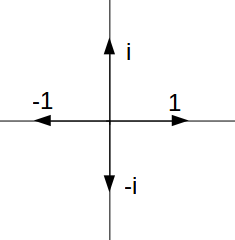
\includegraphics[scale=0.5]{./images/roots.png}
}
\end{figure}

\item En general si $n < 0$ entonces la ecuación $N(x) = a^2 - nb^2 = a^2 + (-n)b^2 = -1$ no tiene solución y debemos considerar sólo las soluciones de $N(x) = a^2 - nb^2 = a^2 + (-n)b^2 = 1$. Para $n = 1$, tenemos el caso anterior y si $n > 1$ entonces es claro que sólo hay dos soluciones que son $1,-1$. 

\item El anillo de los enteros cuadráticos de radicando 2 es $\mathbb{Z}[\sqrt{2}] = \{a+b\sqrt{2}:a,b \in \mathbb{Z}\}$. Este anillo tiene como unidades todas las soluciones $(a,b)$ de las ecuaciones $a^2-2b^2 = 1 \lor a^2-2b^2 = -1$. Obsérvese que como $N(1+ \sqrt{2}) = -1$ entonces $N((1+\sqrt{2})^k) = (-1)^k$ y por tanto todo $(1+\sqrt{2})^k$ son unidades del anillo. Se puede demostrar que todas las unidades del anillo son de esta forma. 

\item En general, el fenómeno del apartado anterior se da para $n > 0$ y al elemento base de las potencias se le llama solución fundamental. 
\end{enumerate}
\end{example}


\pagebreak
\section{Dominios de integridad y cuerpos}
\subsection{Definiciones de dominio de integridad}

\begin{definition}
Un elemento $a \in A$ es divisor de cero si existe $b$ no nulo tal que $ab = 0$. 

Al conjunto de los divisores de cero lo denotaremos por $0_A$.
\end{definition}

\begin{proposition}[Propiedades de $0_A$]
1. En cualquier anillo $A$, $0 \in 0_A$. \\
2. $0_A$ es invariante por isomorfismo. \\
3. Las unidades de un anillo $A$ no pueden ser divisores de cero, esto es, $U(A) \cap 0_A = \emptyset$.
\end{proposition}
\begin{proof}
1. Es evidente.\\
2. Basta observar que un homomorfismo inyectivo lleva unidades de cero en unidades de cero. \\
3. Sea $a \in U(A) \cap 0_A$. Existe $b \neq 0$ tal que $ab = 0$. Multiplicando por el inverso de $a$ obtenemos que $b = 0$. Contradicción.
\end{proof}

\begin{definition}[Dominio de integridad]
Sea $A$ un anillo conmutativo no trivial.

$A$ es un dominio de integridad si y sólo si verifica la propiedad cancelativa, esto es:

$\forall a \in A \setminus \{0\},x,y \in A. ax = ay \implies x = y$. 

o equivalentemente, 

si el único divisor de cero es cero, esto es, $0_A = \{0\}$. 
\end{definition}

La siguiente definición justifica la equivalencia entre ambos criterios:

\begin{proposition}[Equivalencia de las definiciones]
Son equivalentes las siguientes condiciones:

1. $\forall a \in A \setminus \{0\},x,y \in A. ax = ay \implies x = y$. \\
2. $\forall a,b \in A \setminus \{0\}. ab \in A \setminus \{0\}$.
\end{proposition}
\begin{proof}
$\Rightarrow)$ Sean $a,b \in A \setminus \{0\}$ y razonemos por reducción al absurdo que $ab \neq 0$. Si suponemos que $ab = 0$ entonces la ecuación $ax = 0$ tiene dos soluciones $ab = 0$ y $a0 = 0$ en cuyo caso $b = 0$ en contradicción con nuestras hipótesis. 

$\Leftarrow)$ Sean $a \in A \setminus \{0\},x,y \in A$. Supongamos que $ax = ay$. Entonces se verifica que $a(x-y) = 0$. Si $x-y = 0$ hemos terminado ya que entonces $x = y$. En otro caso, $x-y \neq 0$ y tomando $b = x-y$ en 2. tendríamos que $ab \neq 0$ en contradicción con las hipótesis. 
\end{proof}

\begin{proposition}[Propiedades elementales]
1. Todo subanillo de un dominio de integridad es un dominio de integridad.\\
2. La solución de $ax = b$ con $a \neq 0$ en un dominio de integridad, si existe es única.
\end{proposition}
\begin{proof}
	1. Claramente, la propiedad de dominio de integridad se translada a sus subconjuntos y como cualquier subanillo es un anillo se tiene que es un dominio de integridad. \\
	2. En efecto, si $ax_0 = ay_0 \implies x_0 = y_0$. \\
\end{proof}

\begin{example}
	\begin{itemize}
		\item  Por ejemplo los anillos de enteros cuadráticos son dominios de integridad ya que son subanillos del cuerpo de los complejos. 
		
		\item $\mathbb{Z}_6$ no es dominio de integridad ya que la ecuación $2 \cdot x = 0$ tiene más de dos soluciones. Por ejemplo, $x = 3$ y $x = 2$ son solución. 
	\end{itemize}
\end{example}

\begin{proposition}[Propiedades polinómicas]
Sea $A$ un dominio de integridad y consideremos $A[X]$, el anillo de polinomios sobre $A$. 
	
\begin{enumerate}
\item $\forall f,g \in A[X]. grado(fg) = grado(f) + grado(g)$.
\item $A[X]$ es un dominio de integridad.
\item $U(A[X]) = U(A)$
\end{enumerate}
\end{proposition}
\begin{proof}
\begin{enumerate}
\item $f = \sum_{i \ge 0} a_ix^i,g = \sum_{j \ge 0} b_jx^j$ con $grado(f) = n \land grado(g) = m$. Está claro que $grado(fg) \le m + n$ ya que en otro caso, si $grado(fg) > m + n$ entonces $fg = \sum_{k \ge 0} (\sum_{i+j = k} a_ib_j) x^k$ y para $i+j = grado(fg)$ se tiene necesariamente que $i > n \lor j > m \iff a_i = 0 \lor b_j = 0 \implies a_ib_j = 0$.
	
Veamos que el grado es exactamente, $n+m$. El correspondiente coeficiente es $\sum_{i+j = n+m} a_ib_j = a_nb_m$ y ya que $a_n \neq 0 \land b_m \neq 0$ y $A$ es un dominio de integridad, se tiene que $a_nb_m \neq 0$ y por tanto el grado es $n+m$. 

\item Dados $f,g \in A[X] \setminus \{0\}$ con $grado(f) = n \land grado(g) = m$. Por lo anterio, $grado(fg) = n+m$ y dado que ninguno de ellos es nulo claramente, $n,m \ge 0$. Si $n \neq 0 \lor m \neq 0$ entonces $n+m \neq 0$ y por tanto, $fg \neq 0$. Si $n = m = 0$. Dado que $A$ se identifica con un subanillo de $A[X]$ y es un dominio de integridad se tiene también que $fg \neq 0$.

\item $f \in U(A[X]) \iff \exists g \in A[X].fg = 1 \implies gr(fg) = gr(f) + gr(g) = gr(1) = 0 \implies gr(f) = gr(g) = 0 \implies f,g \in U(A)$. Claramente, si $f,g \in U(A)$ entonces también $f,g \in U(A[X])$.
\end{enumerate}
\end{proof}


\subsection{Definición de cuerpo}

\begin{definition}[Cuerpo]
Sea $A$ un anillo conmutativo no trivial. 

$A$ es un cuerpo si $U(A) = A \setminus \{0\}$, es decir, $\forall a \in A \setminus \{0\}.\exists a^{-1}$.
\end{definition}

\begin{definition}[Subcuerpo]
Sea $A$ un cuerpo y $B \subseteq A$. Se dice que B es un subcuerpo de A si $B$ es un subanillo que es un cuerpo. 
\end{definition}

\begin{proposition}[Criterios de subcuerpo]
Sea $A$ un cuerpo y $B \subseteq A$. $B$ es un subcuerpo de $A$ si y sólo si se verifica algunas de las siguientes propiedades:

1. La inclusión $i:B \to A$ es un homomorfismo. \\
2. $B$ es un subgrupo para la suma y el producto. 
\end{proposition}

\begin{proposition}[Caracterización de cuerpo]
Sea $A$ un anillo conmutativo no trivial. Los siguientes son equivalentes:

1. $A$ es un cuerpo. \\
2. $A$ no tiene ideales propios.\\ 
3. Todo homomorfismo no nulo que nace en $A$ es un monomorfismo. 
\end{proposition}
\begin{proof}
\begin{enumerate}
\item Si $A$ es cuerpo e $I$ es un ideal entonces si $I = \langle 0 \rangle$ hemos acabado supongamos existe $x \in I \setminus \{0\}$ entonces como es un cuerpo existe $x^{-1}$ y como es cerrado para productos $xx^{-1} = 1$ y por tanto, el ideal es el total. 

\item Si $A$ no tiene ideales propios entonces dado un homomorfismo $f:A \to B$ su núcleo $Ker(f)$ es un ideal. Como $A$ es no trivial, $1 \notin Ker(f)$ de donde $Ker(f) \neq A$. Por tanto, necesariamente $Ker(f) = \{0\}$, esto es, $f$ es monomorfismo. 

\item Si $A$ no es un cuerpo hemos visto que tendrá ideales propios. Sea $I$ un ideal propio entonces la proyección $p:A \to \frac{A}{I}$ es un homomorfismo no trivial pues existen elementos fuera de $I$ y como $I$ tendrá al menos dos elementos $0 \neq i$ entonces no es inyectiva pues $p(0) = p(i) = 0+I$. 
\end{enumerate}
\end{proof}

\begin{example}[Primeros ejemplos de cuerpos]
1. $\mathbb{Z}_3$ es cuerpo y $\mathbb{R}[X]$,$\mathbb{Z}$ no son cuerpos.\\
2. $\mathbb{Z}$ es un subanillo de $\mathbb{Q}$.\\
3. $\mathbb{Q} \subseteq \mathbb{R} \subseteq \mathbb{C} \subseteq \mathbb{R}[X]$ son subcuerpos.\\
\end{example}

\subsection{Relación entre dominios de integridad y cuerpos}

\begin{proposition}
1. Todo cuerpo es un dominio de integridad.\\
2. Todo dominio de integridad finito es un cuerpo. \\
\end{proposition}
\begin{proof}
1. Si $ax_0 = ax_y0$ con $a \neq 0$ entonces $a^{-1}ax_0 = a^{-1}ay_0$ y por tanto $x_0 = y_0$. \\
2. En efecto, si el dominio $A$ es trivial, se tiene un cuerpo. En otro caso, elijo $a \in A - \{0\}$ y consideramos $\{a^n:n > 1\}$. Claramente, este conjunto se queda en $A$ y por tanto debe ser finito. En particular, deben existir $i > 1$ y $j > 0$ tales que $a^i = a^{i+j}$. Entonces la ecuación $a^ix = a^{i+j}$ tiene al menos dos soluciones $x = 1$ y $x = a^j$, de donde $a^j = 1$ y por tanto $a^{-1} = a^{j-1}$. 
\end{proof}






\pagebreak
\section{Ejemplos de cuerpos}
\subsection{El cuerpo de fracciones de un anillo}

\begin{definition}[Fracciones sobre un dominio de integridad]
Dado un dominio de integridad $A$. 

Llamaremos a cada elemento $(a,b) \in A \times (A \setminus \{0\})$ expresión fraccionaria sobre $A$ de numerador $a$ y denominador $b$. 

Diremos que dos expresiones fraccionarias $(a,b),(c,d) \in A \times (A \setminus \{0\})$ son equivalentes $\iff ad = bc$. Lo denotaremos por $(a,b) \sim (c,d)$. 
\end{definition}

\begin{proposition}[La relación entre expresiones es de equivalencia]
La relación $\sim$ es de equivalencia. 
\end{proposition}
\begin{proof}
La reflexividad y simetría son evidentes. Veamos la transitividad:

$(a,b) \sim (c,d) \land (c,d) \sim (e,f)$ se tiene que $ad = bc \land cf = de$. Por tanto, $afdc = adfc = bcde = bedc$ donde hemos utilizado que el dominio de integridad proviene de un anillo conmutativo. También por ser dominio de integridad, tomando los extremos de la igualdad, se obtiene, $af = be$ o equivalentemente, $(a,b) \sim (e,f)$.  
\end{proof}

\begin{definition}[Cuerpo de fracciones]
Llamaremos fracción de numerador $a$ y denominador $b \neq 0$ a la clase de equivalencia de $(a,b)$ y lo denotaremos por $\frac{a}{b}$. Al conjunto cociente formado por todas estas clases lo llamaremos cuerpo de fracciones y lo denotaremos por $Q(A) = \{\frac{a}{b}:(a,b) \in A \times (A \setminus \{0\})\}$. 

En este conjunto definimos dos operaciones:

\begin{enumerate}
\item Suma de fracciones: $\frac{a}{b} + \frac{c}{d} = \frac{ad+bc}{bd}$.
\item Producto de fracciones: $\frac{a}{b} \cdot \frac{c}{d} = \frac{ac}{bd}$.
\end{enumerate}
\end{definition}

\begin{proposition}[Buena definición de las operaciones sobre el cuerpo de fracciones]
	La suma y el producto de fracciones están bien definidos.
\end{proposition}
\begin{proof}
	Comprobamos que la definición no depende del representante de la clase de equivalencia elegido. En efecto, si $\frac{a_1}{b_1} = \frac{c_1}{d_1} \land \frac{a_2}{b_2} = \frac{c_2}{d_2}$ entonces $\frac{a_1}{b_1}+\frac{a_2}{b_2} = \frac{a_1b_2+a_2b_1}{b_1b_2}$ y $\frac{c_1}{d_1} + \frac{c_2}{d_2} = \frac{c_1d_2+d_1c_2}{d_1d_2}$ luego para comprobar la igualdad bastaría comprobar si $(a_1b_2+a_2b_1)d_1d_2 = (c_1d_2+d_1c_2)b_1b_2$. Esta igualdad se comprueba operando y teniendo en cuenta la igualdad de fracciones: $a_1b_2d_1d_2 + a_2b_1d_1d_2 = c_1d_2b_1b_2 + d_1c_2b_1b_2$ donde se ha usado también la conmutativa del producto. 
	
	Análogamente se comprueba el resto. 
\end{proof}

\begin{proposition}[Caracterización del cuerpo de fracciones]
$(Q(A),+,\cdot)$ es el menor cuerpo que contiene un subanillo isomorfo a $A$.  
\end{proposition}
\begin{proof}
El neutro para la suma es $\frac{0}{1}$ y el opuesto de un $\frac{a}{b}$ es $\frac{-a}{b}$. El elemento neutro del producto es $\frac{1}{1}$ y el elemento inverso de $\frac{a}{b}$ es $\frac{b}{a}$. 

Consideremos el monomorfismo de inmersión canónica $ \lambda: A \to Q(A)$ tal que $\lambda(a) = \frac{a}{1}$. Claramente, $Img(\lambda) = \{\frac{a}{1}:a \in A\}$ y por el primer teorema de isomorfía, $A \cong Img(\lambda)$. Usualmente, se identifica $A$ como subanillo de $Q(A)$ con este isomorfismo. 

Supongamos que $K$ es otro cuerpo que contiene un subanillo isomorfo a $A$. Demostraremos que existe un subcuerpo de $K$ isomorfo a $Q(A)$  y por tanto se tendrá que $Q(A)$ es el menor cuerpo con dicha propiedad. 

Para ello considérese la aplicación $\eta:Q(A) \to K$ tal que $\eta(\frac{a}{b}) = ab^{-1}$. Esta aplicación está bien definida ya que si $\frac{a}{b} = \frac{c}{d}$ entonces $ad = bc$ y por tanto $\eta(\frac{a}{b}) = ab^{-1} = cd^{-1} = \eta(\frac{c}{d})$.  

Además, $\eta$ es un monomorfismo de cuerpos. En efecto, $$\eta\Big(\frac{a}{b} + \frac{c}{d}\Big) = \eta\Big(\frac{ad+bc}{bd}\Big) = (ad+bc)(bd)^{-1} = ab^{-1} + cd^{-1} = \eta\Big(\frac{a}{b}\Big) + \eta\Big(\frac{c}{d}\Big)$$ $$\eta\Big(\frac{a}{b} \cdot \frac{c}{d}\Big) = (ac)(bd)^{-1} = \eta\Big(\frac{a}{b}\Big) \cdot \eta\Big(\frac{c}{d}\Big)$$ $$\eta\Big(\frac{1}{1}\Big) = 1 \cdot 1^{-1} = 1$$ y si $\eta\Big(\frac{a}{b}\Big) = \eta\Big(\frac{c}{d}\Big)$ entonces $(ab^{-1}) = (cd^{-1})$, de donde $ad = bc$ o equivalentemente $\frac{a}{b} = \frac{c}{d}$ (también podía haberse utilizado que todo homomorfismo que sale de un cuerpo es inyectivo). El primer teorema de isomorfía nos dice que $Q(A)$ es isomorfo con $\eta(Q(A))$, que es un subcuerpo de $K$ ya que por ser $\eta$ homomorfismo, es un subanillo y por ser $Q(A)$ un cuerpo, el subanillo es cuerpo. 
\end{proof}

El siguiente resultado reescribe la proposición anterior afirmando que el homomorfismo $\overline{f}$ es universal respecto de todos los monomorfismos que van a cuerpos desde el dominio de integridad de partida, esto es, todos esos monomorfismos factorizan por el cuerpo de fracciones. 

\begin{corollary}[Propiedad universal del cuerpo de fracciones]
	Sea $A$ un dominio de integridad y $K$ un cuerpo, sea $\lambda$ el monomorfismo de inmersión canónica en $Q(A)$. Para todo monomorfismo $f: A \to K$ existe un único homomorfismo $\overline{f}:Q(A) \to K$ tal que $\overline{f} \circ \lambda = f$. Además $Img(\overline{f}) \cong Q(A)$.
	
	\begin{tikzcd}
		A \arrow{r}{f} \arrow{d}{\lambda} &
		K  \\
		Q(A) \arrow[dashed]{ur}[swap]{\overline{f}}
	\end{tikzcd}	

	La aplicación es $\overline{f}(\frac{a}{b}) = f(ab^{-1})$
\end{corollary}
\begin{proof}
	Claramente, $\overline{f} = f \circ \eta$ y por tanto es un homomorfismo y además es fácil que $\overline{f} \circ \lambda = f$. Por tanto, sólo hay que demostrar que es única. 
	
	Si $g$ es otra, entonces $g(\frac{a}{b}) = g(\frac{a}{1} \frac{1}{b}) = (g \circ \lambda)(a) \cdot (g \circ \lambda)^{-1}(b) = f(a)f(b)^{-1} = f(ab^{-1}) = (f \circ \eta)(\frac{a}{b})$ y por tanto, ambas son iguales. 
\end{proof}

\begin{example}
	\begin{enumerate}
		\item Si $K$ es un cuerpo entonces $Q(K) \cong K$
		\item $Q(Q(A)) \cong Q(A)$
		\item El anillo $A$ determina unívocamente el cuerpo de fracciones $Q(A)$ salvo isomorfismo pero puede ocurrir que $Q(A) = Q(B)$ aunque $A,B$ no sean isomorfos. Por ejemplo, $$Q\Big(\{\frac{a}{b}:a,b \in \mathbb{Z} \land \text{ b es impar}\}\Big) = Q(\mathbb{Z}) = \mathbb{Q}$$
	\end{enumerate}
\end{example}

\begin{proposition}[Caracterización alternativa del cuerpo de fracciones]
Dado $A$ un dominio de integridad y $K$ un cuerpo que contiene un subanillo $R$ isomorfo a $A$.

$K \cong Q(A) \iff \forall \alpha \in K. \exists a \in R \setminus \{0\}:a \cdot \alpha \in R$. 
\end{proposition}
\begin{proof}
$\Rightarrow)$ Si $K \cong Q(A) = \{\frac{a}{b}:(a,b) \in A \times (A \setminus \{0\})\}$ entonces dado $\alpha \in K$ sabemos que se corresponde con una fracción $\frac{a}{b} \in Q(A)$ y claramente $\frac{a}{b} \cdot \frac{b}{1} = \frac{a}{1} \in A' \setminus \{0\}$ donde $A' \cong A$ como hemos mostrado en la proposición anterior. Asímismo $A \cong R$ y los elementos distintos de cero se conservan por isomorfismo. Llamemos al elemento imagen de $b$ por isomorfismo $r$. 

Entonces, basta tomar $b \in A \setminus \{0\}$ y se tiene que $\alpha b = \frac{a}{1} \in A'$. Donde hemos utilizado la definición de $A'$ dada en el isomorfismo anterior.  

$\Leftarrow)$ Siempre se verifica que $Q(A)$ es isomorfo a un subcuerpo de $K$, llamémoslo $K'$. Demostraremos que con esta propiedad $K = K'$ y por tanto $K$ es esencialmente el mismo anillo que $Q(A)$ aunque los elementos tengan otros nombres. 

Dado $\alpha \in K$, sabemos que $\exists b \in A \setminus \{0\}$ tal que $b \alpha = \frac{a}{1} \in A'$. Por tanto, $\alpha = ab^{-1} \in K'$. Donde hemos utilizado la definición de $\eta$ de la proposición anterior. 
\end{proof}

\subsection{Cuerpo de racionales cuadráticos}

\begin{definition}[Cuerpo de los racionales cuadráticos]
Para cada $n \in \mathbb{Z}$ que no sea un cuadrado perfecto, se define el conjunto de los racionales cuadráticos de radicando n como $\mathbb{Q}[\sqrt{n}] = \{a+b\sqrt{n}:a,b \in \mathbb{Q}\}$.

A este conjunto se le dota de estructura de anillo mediante las operaciones:

\begin{itemize}
\item Suma: $(a+b\sqrt{n})+(c+d\sqrt{n}) = (a+c) + (b+d)\sqrt{n}$
\item Producto: $(a+b\sqrt{n}) \cdot (c+d\sqrt{n}) = (ac+bdn)+(ad+bc)\sqrt{n}$
\end{itemize}

Dado un racional cuadrático $x = a + b \sqrt{n} \in \mathbb{Q}[\sqrt{n}]$ definimos su conjugado $\overline{x} = a - b \sqrt{n}$ y su norma como $N(x) = x \overline{x} = a^2-nb^2$. Es claro que si $\alpha \in \mathbb{Q}[\sqrt{n}]$ entonces $\alpha^{-1} = \frac{\overline{\alpha}}{N(\alpha)}$.
\end{definition}

Obsérvese que se suele definir $\mathbb{Q}[\sqrt{n}]$ para $n$ libre de cuadrados, esto es, $n$ no es divisible por el cuadrado de ningún entero positivo. Esta condición no es restrictiva ya que $\mathbb{Q}[\sqrt{a^2n}] = \mathbb{Q}[a\sqrt{n}] = \mathbb{Q}[\sqrt{n}]$. (Pregunta: ¿esta condición es relevante en el caso de los $\mathbb{Z}[\sqrt{n}]$?)

\begin{proposition}
Se verifican las siguientes propiedades: 
\begin{enumerate}
\item $\mathbb{Q}$ es un subcuerpo de $\mathbb{Q}[\sqrt{n}] \land \mathbb{Q} = \mathbb{Q}[\sqrt{n}] \iff \text{ n es cuadrado perfecto }$
\item  $\mathbb{Q}[\sqrt{n}]$ es un subanillo de $\mathbb{C}$ y si $n > 0$ entonces $\mathbb{Q}[\sqrt{n}]$ es un subanillo de $\mathbb{R}$. 
\item $-:\mathbb{Q}[\sqrt{n}] \to \mathbb{Q}[\sqrt{n}]$ es un homomorfismo de anillos idempotente.
\item $N:\mathbb{Q}[\sqrt{n}] \to \mathbb{Q}$ es un homomorfismo de grupos multiplicativos.
\item $\mathbb{Q}[\sqrt{n}]$ es el cuerpo de fracciones de $\mathbb{Z}(\sqrt{n})$. En particular, $\mathbb{Z}(\sqrt{n})$ es un subanillo de $\mathbb{Q}[\sqrt{n}]$.
\end{enumerate}
\end{proposition}
\begin{proof}
\begin{enumerate}
\item Trivial. 
\item Trivial.
\item La demostración es la misma que en el caso de los enteros cuadráticos. Nótese sin embargo la diferencia entre los codominios de las aplicaciones norma y conjugado.
\item Ídem
\item Basta ver que todo elemento no nulo admite un inverso. Para ello consideremos que $N(x) = x \overline{x}$ no es nulo salvo que $x$ sea nulo ya que en otro $n$ sería un cuadrado perfecto. Podemos por tanto definir $x^{-1} = \frac{\overline{x}}{N(x)}$ y se tiene que los racionales cuadráticos forman un cuerpo. 
\end{enumerate}
\end{proof}
\pagebreak
\section{Divisibilidad en dominios de integridad}
\subsection{Divisibilidad. Propiedades generales.}

\begin{definition}[Divisores y múltiplos]
Dado un dominio de integridad $A$ y $a,b \in A$.

$a$ es divisor de $b$ o $b$ es múltiplo de $a$ si $\exists c \in A. b = ac$. Lo notamos por $a|b$.

El conjunto de los divisores de $a \in A$ es: $$Div(a) = \{b:b|a\}$$ 
\end{definition}

\begin{proposition}[Relación de divisibilidad para el cero, el uno y las unidades]
Sea $A$ un dominio de integridad. 

\begin{enumerate}
\item $0 \in Div(a) \iff a = 0$ y $Div(0) = A$.
\item $\forall a \in A . 1 \in Div(a) \land Div(1) = U(A)$. 
\item $\forall a \in U(A),b \in A.a \in Div(b) \land Div(a) = Div(1)$ 
\item $\forall a \in A. U(A) \subseteq Div(a)$.
\end{enumerate}
\end{proposition}
\begin{proof}
\begin{enumerate}
\item Claramente, si $a \in A$ entonces $a0 = 0$ de modo que $a|0$ y por tanto, $Div(0) = A$. Por otro lado, si $0|a$ entonces $a = 0c = 0$ y recíprocamente, si $a = 0$ entonces $0 = 00$ de modo que $0 \in Div(a)$. 

\item Dado $a \in A$, como $a = a1$, $1 | a$. Por otro lado, es claro que si $a \in A$ divide a $1$, entonces existe $c \in a$ tal que $ac = 1$, luego $a \in U(A)$ y recíprocamente toda unidad divide por definición al $1$. 

\item Si $a \in U(A)$ entonces para $b \in A$, $b = a(a^{-1}b)$ de modo que $a|b$. Por otro lado, si $c \in Div(a)$ entonces $1 = aa^{-1} = cda^{-1}$ de modo que $c|1$. Recíprocamente si $c \in Div(1)$ entonces $a = cc^{-1}a$ y por tanto, $c \in Div(a)$. 

\item Es consecuencia del apartado anterior. 
\end{enumerate}
\end{proof}

\begin{proposition}[Cálculo con la relación de divisibilidad en dominios de integridad]
Sea $A$ un dominio de integridad. 

1. $a|b \land a|c \implies a|bx+cy$\\
2. $a|b \implies a|bc$\\
3. Si $c \neq 0$ entonces $a|b \iff ac | bc$.\\
4. $a|b \iff ax = b$ tiene una única solución.
\end{proposition}
\begin{proof}
1. $a|b \implies \exists c_1. b = ac_1 \land b|c \implies \exists c_2. c = bc_2$ ahora, $bx + cy = bx + bc_2y = b(x + c_2y) = ac_1(x+c_2y)$ de donde claramente $a | bx+cy$. 

2. $a|b \implies \exists d. b = ad$, ahora, $bc = adc$ y por tanto $a|bc$. 

3. $\Rightarrow)$ $a|b \implies \exists d. b = ad$, ahora, $bc = adc = acd$ y por tanto $ac|bc$. \\
$\Leftarrow)$ $ac|bc \implies \exists d. bc = acd$, ahora, $cb = cad$ y como $A$ es un dominio de integridad se verifica que la ecuación $cx = cad$ admite como mucho una solución ya que $c \neq 0$. Pero aquí tenemos que $b$ y $ad$ son solución y por tanto $b = ad$ de donde $a|b$. 

4. $a|b \iff \exists c \in A. ac = b \iff c$ es solución de $ax = b$. Nótese que en un dominio de integridad si la solución existe es única y por tanto $c$ es la única solución de $ax = b$. 
\end{proof}

\begin{proposition}[Caracterización de la divisibilidad en el cuerpo de fracciones]
Dado un dominio de integridad $A$ y $a,b \in A$ con $a \neq 0$.

Sea $A' \cong A$ con el monomorfismo de inyección canónica en el cuerpo de fracciones. Entonces: $$a|b \iff \frac{b}{a} \in A'$$ 
\end{proposition}
\begin{proof}
$\Rightarrow)$ Si $a|b$ entonces $\exists c. b = ac$ y por tanto $\frac{b}{a} = \frac{c}{1} \in A'$. \\
$\Leftarrow)$ Si $\frac{b}{a} \in A'$ entonces $\exists c \in A. \frac{b}{a} = \frac{c}{1}$ o equivalentemente $b = ac \iff a | b$. 
\end{proof}

\begin{definition}[Elementos asociados]
$b$ está asociado con $a$ si $\exists u \in U(A)$ tal que $ua = b$. Lo denotamos por $a \sim b$. 

El conjunto de asociados de un elemento $a \in A$ es $A(a) = \{ua:u \in U(A)\}$.
\end{definition}

\begin{proposition}[Divisores triviales]
Sea $A$ un dominio de integridad. 

$\forall a \in A. U(A) \cup A(a) \subseteq Div(a)$. 

Los divisores en $U(A) \cup A(a)$ se llaman divisores triviales. 
\end{proposition}
\begin{proof}
Ya vimos que $U(A) \subseteq Div(a)$. Sea $b \in A(a)$, entonces $b = au$ y por tanto, $a = (au)u^{-1}$ de modo que $b = au|a$. 
\end{proof}

\begin{example}[Asociados en algunos anillos]
Veamos como se comporta la relación de asociados en algunos anillos conocidos:

\begin{itemize}
\item En $\mathbb{Z}[i]$, $A(1+i) = \{1+i,-1-i,i-1,1-i\}$.
\item En $\mathbb{Z}[i]$, todo número tiene al menos ocho divisores. 
\item Dado $a \in \mathbb{Z}$, $A(a) = \{a,-a\}$.
\end{itemize}
\end{example}

\subsection{Irreducibilidad}

\begin{definition}[Elemento irreducible de un dominio de integridad]
Sea $A$ un dominio de integridad $a \in A$ es irreducible si:

\begin{itemize}
\item No es cero ni unidad. 
\item Sus únicos divisores son los triviales, esto es, $Div(a) = U(A) \cup A(a)$. 
\end{itemize}
\end{definition}

\begin{proposition}[Caracterización de irreducibles en dominios de integridad]
Dado un dominio de integridad $A$ y $p \in A$ con $p \neq 0 \land p \notin U(A)$. 

p es irreducible $\iff p = ab \implies (a \in U(A) \land b \sim p) \lor (a \sim p \land b \in U(A))$ 

esto es, si p es producto de dos elementos entonces uno es una unidad y el otro es un asociado a p. A este tipo de factorizaciones las llamaremos impropias. 
\end{proposition}
\begin{proof}
$\Rightarrow)$ Supongamos que $p = ab$ y supongamos que $a | p$. Como los únicos divisores de $p$ son los triviales entonces hay dos posibilidades:

\begin{itemize}
\item Si $a = u \in U(A)$ entonces está claro que $b \sim p$. 
\item Si $a = up$ con $u \in U(A)$ entonces $p = upb$ y por ser $A$ un dominio de integridad se tiene que $ub = 1$ luego $b = u^{-1} \in U(A)$. 
\end{itemize}

$\Leftarrow)$ Por contrarrecíproco, si suponemos que $p$ no es irreducible existirá un divisor de $p$ que no es trivial. Esto es, $a|p \land \forall u \in U(A),t \in U(p).a \neq u,t$. Por ser divisor existe $b \in A. p = ab$ y sin embargo $a$ no es trivial. 
\end{proof}

\begin{example}[Ejemplos de irreducibles]
Veamos qué elementos son irreducibles en anillos conocidos:

\begin{itemize}
\item En $\mathbb{Z}$, los irreducibles son los números primos (1 no es primo) y sus opuestos. 

\item En $\mathbb{Z}[\sqrt{n}]$ tenemos condiciones suficientes para determinar si un elemento es irreducible. 

\begin{proposition}[Condición suficiente de irreducibilidad en los enteros cuadráticos]

Dado $\alpha \in \mathbb{Z}[\sqrt{n}]$, si $N(\alpha) = p$ con $p$ irreducible en $\mathbb{Z}$ entonces $\alpha$ es irreducible en $\mathbb{Z}[\sqrt{n}]$.
\end{proposition}
\begin{proof}
En efecto, si $N(\alpha) = p$ con $p$ irreducible entonces si cualquier factorización $\alpha = \beta \gamma$ verificaría que $p = N(\alpha) = N(\beta) N(\gamma)$ y por la caracterización de irreducible en $\mathbb{Z}$ necesariamente $N(\beta) \lor N(\gamma) = 1,-1$ de modo que $\beta \lor \gamma$ sería una unidad y tendríamos la caracterización de irreducible en $ \mathbb{Z}[\sqrt{n}]$.
\end{proof}

Por ejemplo, el elemento $2+3i \in \mathbb{Z}[i]$ sería irreducible ya que $N(2+3i) = 13$ que es irreducible en $\mathbb{Z}$.

Podemos ver que esta condición no es necesaria. Por ejemplo en $\mathbb{Z}[\sqrt{-5}]$ el elemento $\alpha = 1+\sqrt{-5}$ tiene norma $N(\alpha) = 1+ 5 \cdot 1^2 = 6$ que no es irreducible en $\mathbb{Z}$. Sin embargo, $\alpha$ es irreducible ya que si $\alpha = \beta \gamma$ entonces $N(\alpha) = N(\beta)N(\gamma) = 6$ de modo que si quisiéramos que la factorización fuera propia, necesariamente $N(\beta) = 2 \land N(\gamma) = 3$ o $N(\beta) = 3 \land N(\gamma) = 2$. Pero no existen elementos de norma 2 o 3 en $\mathbb{Z}[\sqrt{-5}]$.
\end{itemize}
\end{example}

\subsection{Primalidad}

\begin{definition}[Elemento primo]
Dado un dominio de integridad $A$. $p \in A$ es primo si verifica:

\begin{itemize}
\item No es cero ni unidad.
\item Si $p|ab$ entonces $p|a \lor p|b$. 
\end{itemize}
\end{definition}

\begin{example}[Ejemplos de primos]
Veamos qué elementos son primos en anillos conocidos.

En $\mathbb{Z}[\sqrt{n}]$ tenemos condiciones necesarias para determinar si un elemento es primo. 

\begin{proposition}[Condición necesaria de primalidad en los enteros cuadráticos]
Si $\alpha \in \mathbb{Z}[\sqrt{n}]$ es primo entonces $N(\alpha) = p,-p \lor N(\alpha) = p^2,-p^2$ con $p$ un primo de $\mathbb{Z}$. 

además, si $N(\alpha) = p^2,-p^2$ entonces $\alpha \sim p$ en $\mathbb{Z}[\sqrt{n}]$
\end{proposition}
\begin{proof}
\begin{enumerate}
\item Si $\alpha$ fuera primo en $\mathbb{Z}[\sqrt{n}]$   entonces $N(\alpha) \neq 0,1,-1$ ya que $\alpha$ no es cero ni unidad. Nótese que aquí estamos usando de manera fundamental que $n$ no es un cuadrado perfecto. 

Por tanto, $N(\alpha) = \alpha \overline{\alpha} = \prod p_i$ con $p_i$ primos ya que $\mathbb{Z}$ es un DFU. En particular, $\alpha|p_1 \ldots p_r$ en $\mathbb{Z}[\sqrt{n}]$ y como $\alpha$ es primo, debe dividir a algún factor. 

Si $\alpha|p \implies \exists \beta \in \mathbb{Z}[\sqrt{n}].\alpha \beta = p \implies N(\alpha)N(\beta) = N(p) = p^2 \implies N(\alpha) \in \{p,-p,p^2,-p^2\}$. 

\item Si $N(\alpha) = p^2,-p^2$ entonces claramente, $\alpha \sim p$ ya que entonces $N(\beta) = 1,-1 \implies \beta \in U(\mathbb{Z}[\sqrt{n}])$ y por tanto, $\alpha \sim p$. 
\end{enumerate}
\end{proof}
\end{example}

\begin{proposition}[Relación entre primos e irreducibles en dominios de integridad]
Sea $A$ un dominio de integridad. 

\begin{enumerate}
\item Si $p$ es primo entonces  es irreducible.
\item Si $p$ es irreducible entonces $p$ no es necesariamente primo. 
\end{enumerate}
\end{proposition}
\begin{proof}
\begin{enumerate}
\item Si $p = ab$ veamos que $a \sim 1 \land b \in A(p)$ o $b \sim 1 \land a \in A(p)$. 

En efecto, como $p|p = ab$ y $p$ es primo, sabemos que $p|a \lor p|b$. Supongamos que $p|a$. Entonces como $a|p$ tendríamos que $a \sim p$ y por tanto, $\exists u \in U(A). a = up = uab$ y como $A$ es un dominio de integridad y $a \neq 0$, se sigue que $ub = 1$ esto nos da $b \in U(A)$ y por tanto, la factorización es impropia.

\item Obsérvese que los $\mathbb{Z}[\sqrt{n}]$ son dominios de integridad por ser subanillos de sus cuerpos de fracciones $\mathbb{Q}[\sqrt{n}]$. Por tanto, el conjunto $D = \mathbb{Z}{\sqrt{-5}}$ es dominio de integridad. 

El elemento $a = 1 + \sqrt{-5}$ tiene norma $N(a) = 6$ donde ya vimos que este era un irreducible aunque su norma no era un irreducible de $\mathbb{Z}$. Veamos ahora que este elemento no es primo. 

Como $6 = 2 \cdot 3 = (1+\sqrt{-5})(1-\sqrt{-5})$ se tiene que $1+\sqrt{-5}| 2 \cdot 3$ y sin embargo, $1+\sqrt{-5} \nmid 2,3$ ya que tomando normas, implicaría que $6|4,9$. Contradicción.
\end{enumerate}
\end{proof}

\subsection{Estudio de la relación de asociación}

\begin{proposition}[Caracterización de la relación de asociados]\label{div-1}
Dado un dominio de integridad $A$ y $a,b \in A \setminus \{0\}$. 

1. La relación de ser asociados es una relación de equivalencia. \\
2. $a \sim b \iff a|b \land b|a$.\\
3. $a \sim b \implies Div(a) = Div(b)$.  
\end{proposition}
\begin{proof}
1. En efecto, tenemos que la relación es de equivalencia:

\begin{itemize}
\item $a \sim a$ ya que $a = 1a$.
\item $a \sim b \implies b \sim a$ ya que $b = ua$ entonces $a = u^{-1}b$ y si $u \in U(A)$ entonces también $u^{-1} \in U(A)$. 
\item $a \sim b \land b \sim c \implies a \sim c$ ya que $b = u_1a \land c = u_2b$ entonces $c = u_2 u_1 a$ y $u_1u_2 \in U(A)$ ya que el conjunto de los unidades forma un grupo.  
\end{itemize}

2. Por otro lado, la relación puede ser descrita mediante divisibilidad:

$\Rightarrow)$ Si $a \sim b$ entonces $\exists u \in U(A). b = ua \land a = u^{-1}b$ de donde $a | b \land b | a$. \\
$\Leftarrow)$ Si $a | b$ entonces $\exists c_1 \in A. b = ac_1$ y si $b | a$ entonces $\exists c_2 \in A. a = bc_2$. Entonces $a = a c_1c_2$ y dado que estamos en un dominio de integridad la ecuación $a = ax$ tiene una única solución. Por la anterior $c_1c_2$ es una solución y claramente $1$ es otra solución. Ambas deben ser iguales, es decir, $c_1c_2 = 1$. Esto implica que $c_1 = c_2^{-1}$ y por tanto $a,b$ están asociados.  

3. Está claro que si $a|b \land b|a$ entonces $a$ y $b$ tienen los mismos divisores, ya que si $d|a$ entonces $d|a|b$ y si $d|b$ entonces $d|b|a$. 
\end{proof}

La siguiente proposición describe cuál es la utilidad de la relación de asociados en dominios de integridad. La idea es que la divisibilidad no es un orden sobre un dominio de integridad pero la divisibilidad natural en el cociente de los asociados sí lo es. Esto es lo que se querrá decir en el texto cuando se hable de divisibilidad salvo asociados. La relación de ser asociados también preserva los irreducibles.

\begin{proposition}[Utilidad de la relación de asociados]
Sea $\sim$ la relación ser asociados. 

1. $(A,|)$ es un preorden. $(A,|)$ es un orden $\iff U(A) = \{1\}$.\\
2. $(\frac{A}{\sim},|)$ es un orden donde $|$ es en este caso la relación $[a]|[b] \iff a|b$.\\
3. Si $a \sim b$ con $a,b \in A$ entonces $a$ es irreducible $\iff b$ es irreducible. 
\end{proposition}
\begin{proof}
1. Claramente, $\forall a \in A. a | a$ y $\forall a,b,c \in A. a|b \land b|c \implies a|c$. Observemos que para que se de la propiedad antisimétrica debe verificarse que $\forall a,b \in A. a|b \land b|a \implies a = b$. 

Veamos cuándo se da la antisimétrica. La traducción de $a|b \land b|a$ por la proposición \ref{div-1} es $a \sim b$ para elementos no nulos $a$ y $b$. 

$\Rightarrow)$ Si se da la antisimétrica, entonces si tengo al menos dos elementos no nulos tales que $a|b \land b|a$ entonces sabríamos que $a \sim b$. Si $a = ub$ con $u \in U(A)$ podría ser que $u = 1$ en cuyo caso tendríamos $a = b$. En otro caso, tendríamos $u \neq 1$ y por tanto $b \neq a$ pero en ese caso no tendríamos la antisimetría. Por tanto, necesariamente $U(A) = \{1\}$. Si no tengo al menos dos elementos no nulos tengo los anillos $\{0\}$ o $\{0,a\}$. En el primer caso, está claro que las unidades son $\{0\}$. En el segundo caso, $a = 1$ ya que $0a = 0$ y $aa = a$ ya que en otro caso $a$ sería un divisor de $0$ distinto de $0$. En este dominio claramente, $U(A) = \{1\}$.

$\Leftarrow)$ Si $U(A) = \{1\}$ entonces se da la antisimétrica ya que si $a|b \land b|a$ y $a,b$ son no nulos entonces $a \sim b$ lo que implica que $a = b$. Si uno de ellos es cero, claramente el otro debe ser cero y por tanto también $a = b$.   

2. La relación está bien definida. $$[a] = [a'] \land [b] = [b']  \iff a \sim a' \land b \sim b' \iff a|a' \land a'|a \land b|b' \land b'|b$$ Por tanto $[a]|[b] \iff [a']|[b']$ ya que $a'|a|b|b' \land a|a'|b'|b$. 

Que es reflexiva y transitiva se sigue de las propiedades de $|$ sobre $A$. La antisimetría se sigue del apartado 2. de \ref{div-1}.

3. Claramente, $a = 0 \iff b = 0$ y $a \in U(A) \iff b \in U(A)$ ya que $a \sim b$. Supongamos ahora que $a,b$ no son nulos ni unidades.  

Como $a \sim b \implies a \in A(b)$ de donde $A(a) = A(b)$ y si $a$ es irreducible y $a,b$ son no nulos y no unidades, $Div(a) = U(A) \cup A(a) = U(A) \cup A(b) = Div(b)$ de donde los únicos divisores de $b$ son los triviales y por tanto también es irreducible. El recíproco es análogo. 
\end{proof}

\begin{example}[Anillos con grupo de unidades trivial]
Los ejemplos de anillos $A$ tales que $U(A) = \{1\}$ esto es, el grupo de unidades es trivial no es un clase fácil de determinar \cite{link1}. 

\begin{itemize}
\item $\mathbb{Z}$ no está en esta clase ya que $U(\mathbb{Z}) = \{1,-1\}$.
\item $\prod_i \mathbb{Z}_2$ o $\mathbb{Z}_2[X]$ tienen grupo de unidades tirvial.
\end{itemize}  
\end{example}

\subsection{Máximo común divisor}

\begin{definition}[Máximo común divisor]
Dado un dominio de integridad $A$, $a,b \in A$. $d \in A$ es un máximo común divisor de $a$ y $b$ si:
	
\begin{enumerate}
\item $d | a \land d|b$
\item $\forall c \in A.c|a \land c|b \implies c|d$	\end{enumerate}

Naturalmente, si existe el máximo común divisor $d$ de $a,b$ entonces cualquier otro máximo común divisor $d'$ de $a,b$ sería asociado a él. Ya que por ser $d'$ máximo común divisor $d|d'$ y por serlo $d$, $d'|d$ de modo que $d \sim d'$. Entenderemos que el máximo cómun divisor es único salvo asociados y lo denotaremos por $(a,b)$. Nótese que no siempre tiene que existir.  
\end{definition}

Extendemos la notación Div para conjuntos indicando conjuntos de divisores comunes. Así, $Div(a,b)$ denota los divisores comunes de $a$ y $b$. De ese modo, si $Div(a,b) = Div(a',b')$ entonces trivialmente $(a,b) = (a',b')$.

\begin{proposition}[Propiedades del máximo común divisor]
	En las siguientes propiedades, se entiende que existen los máximos comunes divisores que entran en juego en la igualdad. Las igualdades se dan salvo asociados. 
	
	\begin{enumerate}
	\item Propiedad asociativa: $$(a,(b,c)) = ((a,b),c)$$
	\item Propiedad conmutativa: $$(a,b) = (b,a)$$
	\item Propiedad de supremo: $$(a,0) = a \land (a,1) = 1$$
	\item Relación de divisibilidad: $$a|b \iff mcd(a,b) = a \land a \sim b \iff mcd(a,b) = a = b$$
	\item Linealidad: $$(ac,bc) = (a,b)c$$
	\item Linealidad en el cociente: $$c|a \land c|b \land c \neq 0 \implies \Big(\frac{a}{c},\frac{b}{c}\Big) = \frac{(a,b)}{c}$$
	\item Normalización: $$ a \neq 0 \lor b \neq 0 \implies \Big(\frac{a}{(a,b)},\frac{b}{(a,b)}\Big) = 1$$
	\item Simplificación de numeradores: $$b|ac \implies b|(a,b)c$$
	\item Lema de Euclides: $$(a,b) = 1 \land b|ac \implies b|c$$
	\item Incremento del denominador: $$a|c \land b|c \land (a,b) = 1 \implies ab|c$$
	\item Propiedad del algoritmo de Lagrange: $$(a,bc) = 1 \iff (a,b) = 1 = (a,c)$$
	\item Propiedad del algoritmo de Euclides: $$\forall q \in A.(a,b) = (a-qb,b)$$
	\end{enumerate}
\end{proposition}
\begin{proof}
	\begin{enumerate}
	\item Sea $d \in Div(a,(b,c))$. Tenemos que $d|a \land d|(b,c)$ y como $d|(b,c)$ tenemos que $d|b,c$ por transitividad de la divisibilidad. Como $d|a,b$ también $d|(a,b)$. Reuniendo la información que nos interesa, $d|(a,b),c$ luego $d \in Div((a,b),c)$. 
	
	Un razonamiento análogo da que $Div(a,(b,c)) = Div((a,b),c)$ y por tanto, se tiene la igualdad de los máximo común divisores. 
	 
	\item Si $d \in Div(a,b)$ entonces claramente, $d \in Div(b,a)$. Se tiene que $Div(a,b) = Div(b,a)$ y por tanto se da la igualdad de los máximo común divisores. 
	
	\item Sea $d = (a,0)$. Como $a|0 \land a|a$ tenemos que $a|d$. Pero por hipótesis, $d|a$ de donde $a \sim d$ y podemos escribir $(a,0) = d$. 
		
	Sea  $d = (a,1)$. Como $d|1$ tenemos que $d \in U(A)$ y por tanto, $d \sim 1$ y podemos escribir $(a,1) = 1$.
	
	\item $\Rightarrow)$ Si $a|b$ entonces tenemos las condiciones de máximo común divisor:
	
	\begin{itemize}
	\item $a|a \land a|b$ por hipótesis. 
	\item $d|a \land d|b \implies d|a$ es trivial.
	\end{itemize}
	
	$\Leftarrow)$ Si $mcd(a,b) = a$ entonces por definición de máximo común divisor $a|b$. 
	
	La relación con la relación de asociación es trivial ya que $a \sim b \iff a|b \land b|a$. 
	
	\item Sea $d = (a,b) \land e = (ac,bc)$. 
	
	Si $c = 0$ es trivial.  También, is $d = 0$ entonces $d|a,b \implies a = b = 0$ de modo que la propiedad se sigue. Supongamos que $c,d \neq 0$.
	
	Claramente, $d|a,b \implies dc|ac \land dc|bc \implies dc|e$ de modo que $e = dcu$ con $u \in A$. Terminaremos si demostramos que $u \in U(A)$.
	
	Usando la propiedad de simplificación de los dominios de integridad $(c,d \neq 0)$:
	
	\begin{itemize}
	\item $e|ac \implies \exists x.ac = ex = dcux \implies a = dux$.
	\item $e|bc \implies \exists y.bc 0 ey = dcuy \implies b = duy$
	\end{itemize}
	
	Por tanto, $du|a \land du|b \implies du|d \implies \exists v. d = duv \implies uv = 1 \implies u \in U(A)$. 
	 
	\item Nótese que $a/c,b/c \in A$. Por el apartado anterior $c(a/c,b/c) = (a,b)1 = (a,b) \iff (a/c,b/c) = (a,b)/c$ ya que $c \neq 0$. 
	
	\item Si $(a,b) = 0$ entonces $a = b = 0$ en contradicción con las hipótesis. Entonces tomamos $c = (a,b) \neq 0$ en el apartado anterior y se tiene. 
	
	\item Por definición, $b|ac \implies \exists x.ac = bx$ y entonces $(a,b)c = (ac,bc) = (bx,bc) = b(x,c)$, de modo que $b|(a,b)$. 
	
	\item  Si $(a,b) = 1$ entonces usando el apartado anterior, $b|ac \implies b| (a,b)c = c$. 
	
	\item Como $b|c$, $\exists x. c = bx$. Como $a|c \implies a|bx$ y como $(a,b) = 1$, tenemos que $a|x$. 
	
	Como $a|x$, $\exists y.x = ay \implies c = bay \implies ab|c$. 
	
	\item $\Rightarrow)$ $1 = (a,bc) = ((a,ac),bc) = (a,(ac,bc)) = (a,(a,b)c) = (a,b)(\frac{a}{(a,b)},c) \implies (a,b) \in U(A) \implies (a,b) = 1$
	
	$\Leftarrow)$ $1 = (a,c) = (a,(ac,bc)) = ((a,ac),bc) = (a,bc)$
	\item $Div(a,b) = Div(a-qb,b)$. 
	
	En efecto, si $d \in Div(a,b)$ entonces $d|a,b$ y por tanto, $d$ divide a las combinaciones lineales de $a,b$. En particular, $d|a-qb,b$, esto es, $d \in Div(a-qb,b)$. Recíprocamente, si $d|a-qb,b$ entonces $d$ divide a sus combinaciones lineales y en particular $d|a-qb+qb = a$. Por tanto, $d|a,b$. 
	
	En consecuencia, el máximo divisor de ambos, que existe por hipótesis, es el mismo, esto es, $(a-qb,b) = (a,b)$.  
	\end{enumerate}
	 	
\end{proof}

\begin{example}[El máximo común divisor de cualquier pareja no tiene por qué existir]
Veamos que en $\mathbb{Z}[\sqrt{-5}]$ existe el máximo común divisor para alguna pareja de elementos y no existe para alguna otra pareja de elementos.

\begin{itemize}
\item $\exists (3,1+\sqrt{-5}) = 1$

Observamos que $3$ es irreducible y por tanto, sus divisores son $Div(3) = \{-1,1,-3,3\}$. 

En efecto, si $3 = pq$ de forma propia entonces $N(3)= N(p)N(q) = 9$. Como $N(p),N(q)$ no pueden ser $1,-1$, necesariamente $N(p) = N(q) = 3,-3$ pero la ecuación $a^2+5b^2 = 3$ no tiene solución. 

Se tiene que, $3 \nmid 1+\sqrt{-5}$, ya que $N(1+\sqrt{-5}) = 6$  y si $1+\sqrt{-5} = 3 \alpha$ entonces $6 = 9N(\alpha)$ que no tiene solución. Por tanto, $(3,1+\sqrt{-5}) = 1$.

\item $\nexists (6,2(1+\sqrt{-5}))$

Si suponemos que existe entonces $(6,2(1+\sqrt{-5})) = 2(3,1+\sqrt{-5}) = 2 \cdot 1 = 2$ tendría que ser $2$. 

Para concluir, vemos que $1+\sqrt{-5}|1+\sqrt{-5},6$ ya que:

\begin{itemize}
\item  $(1+\sqrt{-5})(1-\sqrt{-5}) = 6$
\item  $(1+\sqrt{-5})2 = 2(1+\sqrt{-5})$
\end{itemize}

Sin embargo, $1+\sqrt{-5} \nmid 2$, ya que si $1+\sqrt{-5} = 2 \alpha$ entonces $N(2) = N(1+\sqrt{-5})N(\alpha) \implies 4 = 6  N(\alpha)$ lo cual es imposible. 
\end{itemize}
\end{example}

\subsection{Mínimo común múltiplo}

\begin{definition}[Mínimo cómun múltiplo]
Sea $A$ un dominio de integridad y $a,b \in A$. Decimos que $m$ es su mínimo común múltiplo si se verifican las siguientes condiciones:

\begin{enumerate}
\item $a|m \land b|m$
\item $a|c \land b|c \implies m|c$
\end{enumerate}

Naturalmente, si existe el mínimo común múltiplo $m$ de $a,b$ entonces cualquier otro mínimo común múltiplo $m'$ de $a,b$ sería asociado a él. Ya que por ser $m'$ mínimo común múltiplo $m'|m$ y por serlo $m$, $m|m'$ de modo que $m \sim m'$. Entenderemos que el mínimo común múltiplo es único salvo asociados y lo denotaremos por $[a,b]$. Nótese que no siempre tiene que existir.  
\end{definition}

Denotamos por $Mul(a,b)$ a los múltiplos comunes de $a$ y $b$. Si $Mul(a,b) = Mul(a',b')$ entonces trivialmente $[a,b] = [a',b']$ siempre que exista el mínimo común múltiplo.

\begin{proposition}[Propiedades del mínimo común múltiplo]
En las siguientes propiedades, se entiende que existen los mínimos común múltiplos que entran en
juego en la igualdad. Las igualdades se dan salvo asociados.

\begin{enumerate}
\item Propiedad asociativa: $$[[a,b],c] = [a,[b,c]]$$
\item Propiedad conmutativa: $$[a,b] = [b,a]$$
\item Propiedad de ínfimo: $$[a,0] = 0 \land [a,1] = a$$
\item Relación de divisibilidad: $$a|b \iff [a,b] = b \land a \sim b \iff [a,b] = a = b$$
\item Linealidad: $$[ac,bc] = [a,b]c$$
\item Relación ínfimo-supremo: $\exists [a,b] \implies \exists (a,b) \land [a,b](a,b) = ab$. 
\end{enumerate}
\end{proposition}
\begin{proof}
\begin{enumerate}
\item Sea $m \in Mul([a,b],c)$.  Entonces claramente, $m$ es múltiplo de $a,b,c$ y por tanto, $m$ es múltiplo de $[b,c]$ y de $a$ de modo que $m \in Mul(a,[b,c])$. 

Razonando de forma análoga se llega a que $Mul([a,b],c) = Mul(a,[b,c])$ de donde se tiene el enunciado.  

\item Claramente, $Mul(a,b) = Mul(b,a)$ y por tanto, se tiene el enunciado. 

\item Observamos que $Mul(a,0) = \{0\}$ y como $0|0$, necesariamente, se tiene que $[a,0] = 0$. 

Por otro lado, $Mul(a,1) = \langle a \rangle$ y es claro que si $c \in \langle a \rangle$ entonces $a|c$. De aquí que $[a,1] = a$. 

\item $a|b \iff \exists c.b = ac \iff \langle b \rangle \subseteq \langle a \rangle \iff Mul(a,b) = \langle b \rangle \iff [a,b] = b$. 

$a \sim b \iff \exists u \in U(A).b = au \land a = u^{-1}b \iff \langle b \rangle = \langle a \rangle \iff Mul(a,b) = \langle a \rangle = \langle b \rangle \iff [a,b] = a = b$.

\item Si $c = 0$, la propiedad es trivial, $[0,0] = 0 = 0 [a,b]$. Supongamos que $c \neq 0$ y veamos que $Mul(ac,bc) = cMul(a,b)$. En efecto, si tomo $m \in Mul(ac,bc)$ entonces $m = acd = bcd'$ y como $c \neq 0$, $ad = bd'$ lo que implica que $m \in cMul(a,b)$. Recíprocamente, si $m \in cMul(a,b)$ entonces $m = cad = cbd'$ de donde claramente, $m \in Mul(ac,bc)$. 

En consecuencia, $ac,bc|c[a,b]$ y si $ac,bc|m$ entonces $m = cad = cbd'$ de donde obviamente, $c[a,b]|m$. 

\item Obsérvese que en el caso $a = 0 \lor b = 0$ las existencias son triviales y la igualdad también. Por tanto, supongamos que $a,b \neq 0$. 

La estrategia es observar que $ab$ es un múltiplo común de $a,b$ y que como existe $m = [a,b]$ podemos escribir $ab = md$. Nuestro objetivo es demostrar que $d = (a,b)$. 

\begin{enumerate}
\item Como $a,b|[a,b]$, $\exists a_1,b_1.m = a_1a = b_1b$ y entonces $ab = md = a_1ad = b_1bd$ y como estamos en un dominio de integridad, $b = b_1d \land a = a_1d \implies d|a,b$. 

\item Supongamos que $d_1|a,b$. Entonces, $\exists m_1. m_1d_1 = ab$. Además, $a|m_1,b|m_1 \implies m|m_1 \implies \exists c. m_1 = cm$. Por tanto, $md = ab = m_1d_1 = d_1mc$ y simplificando, $d = d_1c \implies d_1|d$. 

Obsérvese que hemos utilizado que $m \neq 0$ para simplificar. Esto se deduce de que si $0 = [a,b]$ entonces como $[a,b]|ab \implies ab = 0$ pero por hipótesis $a,b \neq 0$ y como estamos en un dominio de integridad, $ab \neq 0$. Contradicción.
\end{enumerate}
\end{enumerate}
\end{proof}

Curiosamente, la existencia de máximo común divisor no garantiza la existencia de mínimo común múltiplo. 

\begin{example}[Existencia de mcd no implica existencia de mcm]
Sea $A = \{a_0+2a_1x+\ldots:a_i \in \mathbb{Z} \} \subseteq \mathbb{Z}[X]$ el conjunto de los polinomios con coeficientes enteros que en grado 1 tienen coeficiente par. Claramente, $A$ es cerrado para sumas y productos y además contiene al uno. Por tanto, al ser subanillo de un dominio de integridad, también será un dominio de integridad. 

Calculemos $(2,2x)$. Los divisores de 2 son $1,-1,2,-2$ ya que $2$ es irreducible. Un divisor común para ambos tiene que estar en esta lista. Sin embargo, $2 \nmid 2x$ en $A$ ya que tendría que verificarse la ecuación: $$2x = 2(a_0+2a_1x+\ldots) = 2a_0+4a_1x+\ldots$$ Claramente, la única posibilidad es que el divisor común sea $1$ o $-1$ y como el máximo común divisor es único salvo asociados, $(2,2x) = 1$. 

Podemos comprobar que $\nexists [2,2x]$. Por reducción al absurdo, si existiese $[2,2x]$ entonces existiría $(2,2x)$ (que de hecho existe) y además $[2,2x](2,2x) = 4x$. Como $(2,2x) = 1$, tendrá que ser $[2,2x] = 4x$. 

Consideremos el elemento $2x^3 = (2)(x^3) = (2x)(x^2)$. Claramente, $2|2x^3$ y $2x|2x^3$. Por definición de mínimo común múltiplo, debería verificarse que $4x|2x^3$ y en particular, $2x^3 = 4x(a_0+2a_1x+a_2x^2+\ldots)$. La ecuación que se obtiene en grado 3 es, $2 = 4a_2$ que no tiene solución entera. 
\end{example}

\begin{proposition}[Existencia de mcd implica la de mcm]
Sea $A$ un dominio de integridad. 

Si existe el máximo común divisor de cualquier par de elementos entonces existe el mínimo común múltiplo de cualquier par, esto es, $\forall a,b \in A. \exists (a,b) \implies \forall a,b \in A. \exists [a,b]$.
\end{proposition}
\begin{proof}
Sean $a,b \in A \setminus \{0\}$ y $d = (a,b)$. Como $d|a,b$ también $d|ab$ y como no podía ser de otro modo eligiremos $m = \frac{ab}{d}$ como candidato a ser $[a,b]$.

\begin{enumerate}
\item Como $m = \frac{ab}{d} = a \frac{b}{d} = ab_1 \land  m = \frac{ab}{d}= \frac{a}{d}b = a_1b$ es claro que $a|m \land b|m$. 
\item Sea $m_1 \in A$ tal que $a|m_1 \land b|m_1$. Queremos ver que $m|m_1$. Para ello tomo $k = (m,m_1)$ que existe por las hipótesis y elijo $d_1 = \frac{m}{k} \in A$. 

Como $a|m \land a|m_1$ se tiene que $a|k$ y análogamente $b|k$. Sea $k = au = bv$. Tenemos: $$m = a_1b = kd_1 = bvd_1\implies a_1 = vd_1 \implies a = da_1 = vdd_1$$ $$m = b_1a = k d_1 = aud_1 \implies b_1 = ud_1 \implies b = db_1 = ud_1d$$ Por tanto, $$dd_1|a,b \implies dd_1 |d1 \implies d_1|1 \implies d_1 \in U(A)$$ Como $m = kd_1$ tenemos que $m = (m,m_1)$ luego $m|m_1$ como queríamos. 
\end{enumerate}

\end{proof}

\subsection{Invarianza de la divisibilidad frente a isomorfismos}

Nos ocupamos ahora de hacer explícito una noción que sería evidente. Los isomorfismos de anillos no pueden distinguir los conceptos anteriores. Sin embargo, lo hacemos aquí explícito porque al menos nos hará falta cuando hablemos del criterio de irreducibilidad por traslación. 

\begin{proposition}
Sea $f:A \to B$ un isomorfismo de anillos. 

\begin{enumerate}
\item El conjunto de los divisores es invariante por $f$. 
\item Los elementos asociados son invariantes por $f$. 
\item La irreducibilidad de un elemento es invariante por $f$. 
\end{enumerate}
\end{proposition}
\begin{proof}
\begin{enumerate}
\item $d|a \implies a = dc \implies b = f(d)f(c) \implies f(d)|b \implies f(Div(a)) \subseteq Div(b)$

$d'|b \implies b = d'c' \implies a = f^{-1}(b) = f^{-1}(d')f^{-1}(c') \implies f^{-1}(d') | a \implies Div(b) \subseteq f(Div(a))$. 

\item Ya sabemos que las unidades son invariantes por $f$. Entonces: $$f(A(a)) = f(aU(A)) = f(a)f(U(A)) = bU(B) = A(b)$$

\item $f$ preserva unidades y el cero. Por tanto, si $a$ no es cero ni unidad entonces $f(a)$ no es cero ni unidad. Como los divisores y los divisores triviales se preservan, tenemos que los irreducibles se preservan. 
\end{enumerate}
\end{proof}
























\pagebreak
\section{Dominios euclídeos}
\subsection{Definición y propiedades generales}

\begin{definition}[Dominio euclídeo]
	Un dominio de integridad $A$ es un dominio euclídeo si existe una función euclídea $\phi:A \setminus \{0\} \to \mathbb{N}$ tal que:
	
	\begin{enumerate}
	\item $\forall a,b \in A \setminus \{0\}. \phi(ab) \ge \phi(b)$
	\item $\forall a,b \in A,b \neq 0. \exists q,r \in A. a = bq + r$ con $r = 0$ o $\phi(r) < \phi(b)$.
	\end{enumerate}
	
	En la propiedad anterior, $q$ se llama cociente y $r$ se llama resto. La segunda condición puede restringirse a la comprobación de la siguiente propiedad: 
	
	$\forall a,b \neq 0. \phi(a) \ge \phi(b). \exists q,r \in A. a = bq + r$ con $r = 0$ o $\phi(r) < \phi(b)$
	
	con lo que nos quitamos los casos $a = b0 + a \land 0 = b0 + 0$. Equivalentemente:
	
	$\forall a,b \neq 0. \phi(a) \ge \phi(b). \exists q \in A. a = bq \lor \phi(a-bq) < \phi(b)$
\end{definition}

\begin{example}[Cualquier cuerpo es un dominio euclídeo]

En efecto, si $K$ es un cuerpo, la función euclídea es $\phi: K \setminus \{0\} \to \mathbb{N}$ tal que $\phi(k) = 1$. 

Se verifica que $\forall a,b \in A \setminus \{0\}.\phi(ab) \ge \phi(b)$. Además, $\forall a,b \in A, b \neq 0. q = a b^{-1} \land r = 0 \implies a = qb + r$.
\end{example}

\begin{proposition}[Caracterización de la divisibilidad en dominios euclídeos]
	Dado $A$ un dominio euclídeo. 
	
	$b | a \iff \exists q \in A. a = bq$ esto es, todo resto euclídeo de la división de $a$ entre $b$ es cero. 
\end{proposition}
\begin{proof}
	$\Rightarrow)$ Como $b|a \implies \exists c \in A. a = bc$ y como $A$ es un dominio euclídeo $\exists q,r. a = bq + r$ con $r = 0 \lor \phi(r) < \phi(b)$. Si $r = 0$ hemos acabado. En otro caso, suponemos $r \neq 0$ y por tanto debe ser $\phi(r) < \phi(b)$. 
	
	Claramente, $bc = bq + r $ y por tanto $r = b(c-q)$. Tomando $\phi$, tenemos que $\phi(r) = \phi(b(c-q)) \ge \phi(b) > \phi(r)$ por hipótesis y llegamos a una contradicción. Por tanto debe ser, $r = 0$. 
	
	$\Leftarrow)$ Trivial. 
\end{proof}

\subsection{Dominio euclídeo de los enteros}

\begin{theorem}[Teorema de Euclides]
$\mathbb{Z}$ es un dominio euclídeo con:
	
\begin{enumerate}
\item Función euclídea el valor absoluto. 
\item Unicidad del cociente y unicidad  del resto sobre $\mathbb{N}$. 
\end{enumerate} 
	
hay que notar que la unicidad de este resultado es impuesta en el sentido de que los restos son únicos si sólo se consideran válidos sobre $\mathbb{N}$ y no sobre $\mathbb{Z}$ como permite la definición de dominio euclídeo. 
\end{theorem}
\begin{proof}
	1. Claramente, $\forall a,b \in A. \phi(ab) = |ab| \ge |b| = \phi(b)$.\\
	2. Sea $b > 0$ y consideremos el conjunto de posibles restos positivos que pueden quedar al dividir por $b$, esto es, $R = \{a-bx:x\in \mathbb{Z}\} \cap \mathbb{N}$. Vamos a elegir como $r$ el mínimo de este conjunto. 
	
	Primero vemos que $R \neq \emptyset$. Para ello basta elegir $x = - |a|$ de modo que el correspondiente elemento del conjunto es $a + b|a|$. Distinguimos dos casos:
	
	\begin{itemize}
		\item Si $a > 0 \implies a+b|a| = a+ba = a(1+b) \ge 0$.
		\item Si $a < 0 \implies a+b|a| = a-ba = a(1-b) \ge 0$. 
	\end{itemize}
	
	Por tanto $a+b|a| \in R$ y como $\mathbb{N}$ es bien ordenado tenemos que $R$ tiene un mínimo. Definimos $r = min R$. Como $r \in R$ claramente $r \ge 0$ y $\exists q \in \mathbb{Z}. r = a-bq \implies a = bq + r$. Terminamos la demostración para este caso, garantizando que $r < |b| = b$. Pero esto es fácil ya que si $r \ge b$ entonces $r-b = a-b(q+1) \implies r-b \in R$ y como $r-b < r$ tenemos contradicción con la definición de $r$. Por tanto se verifica que $r < |b|$. 
	
	Si $b < 0$ entonces se transforma al caso $b > 0$. Se resuelve el problema para $a$ y $-b$ obteniendo una expresión $a = (-b)q+r$ con $0 \leq r < |-b|$ de donde $a = b(-q) + r$ y claramente $0 \leq r < |b|$ ya que $|-b| = |b|$. 
	
	Finalmente, veamos que el cociente y el resto son únicos.  Para ello escribamos $$a = bq + r = bq'+r' \text{ con } 0 \le r < |b| \land 0 \le r' < |b| \implies b(q'-q) = r' - r \implies |b| \le |q' - q||b| = |r'-r|$$ donde la última desigualdad se cumple por el carácter multiplicativo del valor absoluto. Obsérvese que estamos asumiendo implícitamente que $q \neq q' \land r \neq r'$ para poder tomar valores absolutos en la definición de dominio euclídeo. Si los cocientes son iguales es fácil deducir que los restos son iguales y viceversa teniendo en cuenta que $\mathbb{Z}$ es un dominio de integridad. 
	
	Sin embargo, por las condiciones que cumplen $r$ y $r'$ tendríamos que: $$0 \le r < |b| \land -|b| < -r' \le 0 \implies -|b| < r' - r < |b| \implies |r'-r| < |b|$$ Ambas desigualdades son contradictorias.
\end{proof}

El conjunto $R = \{a-bx:x \in \mathbb{Z}\} \cap \mathbb{N}$ no es directamente computable. Pero si $a,b > 0$ bastaría con comprobar una lista de números naturales comenzando en cero para hallar el menor elemento del conjunto (que existe y es único por el teorema anterior). Entonces conviene definir el siguiente procedimiento algorítmico para calcular los restantes casos:

\begin{theorem}[Algoritmo de división]
	\begin{itemize}
		\item Si $a,b > 0$ se procede del modo habitual. 
		\item En otro caso los resultados se obtienen al dividir los correspondientes positivos:
		\begin{itemize}
			\item Si $r = 0 \land a = bq$
			
			\begin{itemize}
				\item Si $a,b < 0$ entonces $-a = (-b)q$
				\item Si $a < 0$ entonces $-a = b(-q)$
				\item Si $b < 0$ entonces $a = (-b)(-q)$.
			\end{itemize}
			\item Si $r > 0 \land r < b, a = bq+r$
			
			\begin{itemize}
				\item Si $a,b < 0$ entonces $-a = (-b)(q+1)+(b-r)$.
				\item Si $a < 0$ entonces $-a = b(-q-1)+(b-r)$.
				\item Si $b < 0$ entonces $a = (-b)(-q)+r$. 
			\end{itemize}
		\end{itemize}
	\end{itemize}
\end{theorem}

\subsection{Dominio euclídeo de los polinomios con coeficientes en un cuerpo.}

\subsubsection{Demostración basada en un algoritmo de división sobre dominios de integridad}

\begin{lemma}[División de polinomios en dominios de integridad]
	Dado $A$ un dominio de integridad. 
	
	$\forall f,g \in A[X]$ donde el coeficiente líder de $g$ es unidad del anillo, $\exists!q,r \in A[X]. f = gq + r$ con $r = 0$ o $gr(r) < gr(g)$. 
\end{lemma}
\begin{proof}
	Sean $f = \sum_{i=0}^{n} a_ix^i$ con $a_n \neq 0$ y $g = \sum_{i = 0}^{m} b_jx^j$ con $b_m \in U(A)$. Ahora, 
	
	\begin{itemize}
		\item Si $n < m$ entonces $f(x) = g(x)0 + f(x)$. 
		\item Si $n \ge m$ entonces hacemos inducción fuerte sobre $n$. 
		
		\begin{itemize}
			\item Si $n = 0$ entonces $f = a_0 \land g = b_0 \in U(A)$ y por tanto podemos escribir $f = a_0 = b_0(b_0^{-1}a_0) + 0$. 
			\item Si $n > 0$ podemos considerar $f_1 = f - a_nb_m^{-1}x^{n-m}g$ esto es el polinomio que resulta al restar apropiadamente el divisor $g$ poniendole como coeficiente el coeficiente de grado $n$ del polinomio $f$. Claramente, $gr(f_1(x)) < gr(f(x))$ y por hipótesis de inducción $\exists!q_1,r_1 \in A[X]. f_1 = gq_1+r_1$ con $r_1 = 0$ o $gr(r_1) < gr(g)$. 
			
			Usando la anterior descomposición hallamos la descomposición para $f$ como: $$f = f_1(x) = a_1b_m^{-1}x^{n-m}g = gq_1 + r_1 + a_nb_m^{-1}x^{n-m}g = g(q_1+a_nb_m^{-1}x^{n-m}+r_1$$ Y llamamos $q = q_1+a_nb_m^{-1}x^{n-m} \land r = r_1$ y por tanto $r = 0 \lor gr(r) < gr(g)$.  
		\end{itemize}
	\end{itemize}
	
	Finalmente, mostramos que $q,r$ son únicos. En efecto, si $f = gq+r = gq'+r'$ con $r = 0 \lor gr(r) < gr(g)$ y $r' = 0 \lor gr(r') < gr(g)$ entonces $r'-r = g(q-q')$. Si asumimos que $q = q'$ entonces también $r = r'$ y hemos acabado. Si por otra parte asumimos $q \neq q'$ entonces está claro que $gr(r'-r) < gr(g(q-q'))$ ya que $gr(r),gr(r') < gr(g) \land gr(q-q') > 0$. Por tanto, el miembro derecho tiene grado mayor que $g$ y el miembro izquierdo menor que $g$. Esto es una contradicción. Se deduce que hay unicidad. 
\end{proof}

\begin{theorem}[Polinomios sobre un cuerpo forman un dominio euclídeo]
	Dado un cuerpo $K$. El anillo de polinomios sobre $K$, $K[X]$, es un dominio euclídeo con:
	
	\begin{enumerate}
	\item Función euclídea el grado.
	\item Unicidad de cocientes y restos. 
	\end{enumerate} 
\end{theorem}
\begin{proof}
	1. Por ser $K$ un dominio de integridad se tiene que: $$\forall f,g \in K[X] \setminus \{0\}.gr(f \cdot g) = gr(f) + gr(g) \ge gr(g)$$
	
	2. La propiedad se verifica por el lema anterior. Obsérvese que la condición \textit{el coeficiente líder es una unidad del anillo} no es restrictiva en el caso de un cuerpo. 
\end{proof}

\begin{example}
	\begin{itemize}
		\item $\mathbb{R}[X]$ es un dominio euclídeo. 
		\item No son dominios euclídeos, $\mathbb{Z}[\sqrt{5}],\mathbb{Z}[X],\mathbb{R}[X,Y]$
	\end{itemize}
	
	Para resolver $(2+3x+4x^2)z = 2+3x+4x^3+2x^4$ en $\mathbb{Z}_5[X]$ realizamos el procedimiento de división de la demostración del lema anterior:
	
	$$2x^4+4x^3+3x+2 = (3x^2)(4x^2+3x+2) + (4x^2+3x+2)$$
	$$(4x^2+3x+2) = (4x^2+3x+2)1$$
	
	Y se obtiene $z = 3x^2+1$. 
\end{example}

\subsubsection{Demostración basada en un algoritmo de pseudo-división sobre anillos conmutativos}

Sea $A$ un anillo conmutativo.

Damos ahora un procedimiento de pseudo-división que generaliza el procedimiento de división anterior y que se debe al matemático Wu Wen-Tsiin (cuando este algoritmo se considera sobre polinomios multivariados).

En lo sucesivo denotaremos $cl(f) \in A$ al coeficiente líder del polinomio $f$, esto es, el coeficiente no nulo de mayor grado. 

Es claro que $\forall f \in A[X] \setminus \{0\}$ podemos escribir $f = cl(f)X^{gr(f)}+\underline{f}$ con $gr(\underline{f}) < gr(f)$ donde $cl(f)X^{gr(f)}$ es el término en grado $gr(f)$ del polinomio $f$. 

Esta notación es útil si se quiere probar el siguiente lema:

\begin{lemma}[Cotas para el grado de las operaciones con polinomios]
Sean $f,g \in A[X]$ entonces:

\begin{enumerate}
\item $gr(f+g) \le max(gr(f),gr(g))$
\item $gr(fg) \le gr(f) + gr(g)$ y $gr(fg) = gr(f) + gr(g) \iff cl(f)cl(g) \neq 0$. 
\end{enumerate}
\end{lemma}

\begin{theorem}[Pseudo-división en anillos conmutativos]
Dados $f,g \in A[X]$ con $g \neq 0,gr(f) \ge gr(g)$ y $A$ un anillo conmutativo cualquiera. Entonces $ \exists l \ge 0,q,r \in A[X]$ tales que $cl(g)^lf = qg+r$ con $r = 0 \lor gr(r) < gr(g)$ (se puede enunciar considerando que por convención la primera condición está contenida en la segunda). A $q$ se le suele llamar pseudo-cociente y a $r$ pseudo-resto de la división.
\end{theorem}
\begin{proof}
Consideramos el siguiente algoritmo:

Como entrada, tomamos dos polinomios $f,g \in A[X]$ con $g \neq 0$ y $gr(f) \ge gr(g)$, donde reordenamos los polinomios si fuera necesario. Como salida obtendríamos los valores $l \ge 0,q,r \in A[X]$ del enunciado. Inicializamos $q = 0,l = 0,r = f$.

En cada paso si $gr(r) \ge gr(g) \land r \neq 0$ (la segunda condición podemos por convención verla como un caso de la primera). Queremos, como en la división euclídea eliminar uno a uno los términos de $r$, para ello se actualiza $r = cl(g)r - cl(r)X^{gr(r)-gr(g)}g$. Previamente a esta actualización, pero intuitivamente basándonos en ella, queremos determinar un cociente adecuado. Para tener la ecuación deseada tenemos en cuenta el cociente euclídeo usual (que corresponde al segundo sumando anterior) y una factor escalado del cociente anterior, resulta $q = cl(g)q + cl(r)X^{gr(r)-gr(g)}$. En cada paso, el factor de escala $l$ se aumenta en $1$.

Observemos que si $g \neq 0$ el algoritmo genera dos sucesiones de polinomios $q_l,r_l \in A[X]$ de la forma:

\begin{center}
  \begin{tabular}{ | l | c | r |}
    \hline
    $l$ & $q_l$ & $r_l$  \\ \hline
    0 & 0 & f          \\ \hline
     & \ldots & \ldots          \\ \hline
    $l+1$ & $q_{l+1} = cl(g)q_l + cl(r_l)X^{gr(r_l)-gr(g)}$ & $r_{l+1} = cl(g)r_l - cl(r_l)X^{gr(r_l)-gr(g)}g$ \\ \hline
  \end{tabular}
\end{center}

Podemos razonar por decenso infinito sobre el grado de los restos que el algoritmo para:

Por hipótesis, $gr(r) \ge gr(g)$ y por tanto, como inicialmente $r = f$, el algoritmo debe entrar al menos una vez en el bucle principal. Veamos que en cada paso disminuye el grado del pseudo-resto parcial: $$r_{l+1} = cl(g)r_l - cl(r_l)X^{gr(r_l)-gr(g)}g = cl(g)(cl(r_l)X^{gr(r_l)} \underline{r_l}) - cl(r_l)X^{gr(r_l)-gr(g)}(cl(g)X^{gr(g)}+\underline{g}) = cl(g)\underline{r_l} - cl(r_l)\underline{g}$$ Por tanto, $gr(r_{l+1}) = gr(cl(g)\underline{r_l} - cl(r_l)\underline{g}) \le max(gr(\underline{r_l}),gr(\underline{g})) < gr(r_l)$. En consecuencia, el algoritmo para. Veamos ahora por inducción, que para con la respuesta correcta:

Si $l = 0$ entonces $cl(g)^lf = f = 0g + f = q_0g+r_0$. Suponiendo que la ecuación es cierta para $l$, lo comprobamos para $l+1$: $$q_{l+1}g+r_{l+1} = (cl(g)q_l + cl(r_l)X^{gr(r_l) - gr(g)})g + (cl(g)r_l - cl(r_l)X^{gr(r_l) - gr(g)}g) = $$ $$ = cl(g)q_lg + cl(g)r_l =cl(g)(q_lg+r_l) = cl(g)cl(g)^lf = cl(g)^{l+1}f$$ En consecuencia, el algoritmo, que eventualmente termina, lo hace con la respuesta correcta y $r = 0 \lor gr(r) < gr(g)$.
\end{proof}

\begin{example}[Ejemplo de pseudo-división]
En $\mathbb{Z}[X]$ pseudo-dividir $f = 3X^3+5X+1$ entre $g = 2X+1$. 

\begin{center}
  \begin{tabular}{ | l | c | r |}
    \hline
    $l$ & $q_l$ & $r_l$  \\ \hline
    $0$ & $0$ & $3X^3+5X+1$ \\ \hline
    $1$ & $3X$ & $-3X^2 + 5X + 1$ \\ \hline
    $2$ & $6X^2-3X$ & $23X+4$ \\ \hline
    $3$ & $12X^2-6X+23$ & $-15$ \\ \hline
  \end{tabular}
\end{center}

Por tanto, la pseudo-divisón resulta $2^3(3X^3+5X+1) = (12X^2-6X+23)(2X-1) - 15$
\end{example}

\begin{corollary}[Polinomios sobre un cuerpo forman un dominio euclídeo]
Sea $K$ un cuerpo, entonces $K[X]$ es un dominio euclídeo con función euclídea el grado. 
\end{corollary}
\begin{proof}
La primera condición se comprueba como en el caso de la división euclídea. La segunda condición utiliza la pseudo-división. En efecto, dados $f,g \in K[X]$ con $g \neq 0$ tendríamos que $\exists l \ge 0,q,r \in K[X].cl(g)^l f = qg + r$ con $r = 0 \lor gr(r) < gr(g)$. Dado que $cl(g)^l \neq 0$, es invertible y por tanto, $f = cl(g)^{-l}qg+cl(g)^{-l}r$ y si donde los valores obtenidos son el único resto y el único cociente admitidos en la división euclídea ya que $gr(cl(g)^{-l}r) = 0 \lor gr(cl(g)^{-l}r) = gr(r) < gr(g)$. 
\end{proof}

Como ejercicio, podríamos adaptar el algoritmo extendido de Euclides para usar sólo pseudo-divisiones, para ello bastaría adaptar los $u_i,v_i$. 

\subsection{Dominio euclídeo de los enteros cuadráticos}

\begin{theorem}[Algunos enteros cuadráticos forman dominios euclídeos]
	Si $n = -2,-1,2,3$ el anillo $\mathbb{Z}[\sqrt{n}]$ es un dominio euclídeo con:
	
	\begin{enumerate}
	\item Función euclídea el valor absoluto de la norma.
	\item No se garantiza la unicidad de cocientes y restos de la división.  
	\end{enumerate} 
\end{theorem}
\begin{proof}
	La expresión de la función euclídea es $\phi(a+b\sqrt{n}) = |N(a+b\sqrt{n})| = |a^2 - nb^2|$.
	
	\begin{enumerate}
	\item Veamos que $\forall \alpha,\beta \in \mathbb{Z}[\sqrt{n}] \setminus \{0\}.\phi(\alpha \beta) \ge \phi(\alpha)$. 
	
	En efecto, como la norma es un homomorfismo multiplicativo, se tiene que: $$\phi(\alpha \beta) = |N(\alpha \beta)| = |N(\alpha) \cdot N(\beta)| = |N(\alpha)||N(\beta)| = \phi(\alpha)\phi(\beta) \ge \phi(\alpha)$$ La última desigualdad se da ya que $\alpha,\beta \neq 0$ por hipótesis.
	
	\item Veamos ahora que $\forall \alpha,\beta \in A \setminus \{0\}, |N(\alpha)| \ge |N(\beta )|. \exists q,r. \alpha = \beta q+r$ con $r = 0 \lor |N(r)| < |N(b)|$ que era una de las expresiones de la segunda condición. 
	
	Observemos que queremos conseguir $\alpha = \beta q + r$ idealmente tendremos $\alpha = \beta q$ pero en otro caso lo que tendremos será una aproximación del racional cuadrático $\frac{\alpha}{\beta} = a_1 + a_2 \sqrt{n} \in \mathbb{Q}[\sqrt{n}]$ con $a_1,a_2 \in \mathbb{Q}$. Para trabajar con expresiones convenientes de $a_1,a_2$ debemos racionalizar ($\frac{\alpha}{\beta} = \frac{\alpha \overline{\beta}}{N(\beta)}$).
	
	Sean entonces $q_1,q_2 \in \mathbb{Z}$ los enteros que más se aproximan a $a_1,a_2$, esto es: $$|a_1-q_1| \le \frac{1}{2} \land |a_2 - q_2| \le \frac{1}{2}$$ donde si alguna coordenada está justo en la mitad se elige un entero o el siguiente indistintamente. Formamos el entero cuadrático cociente $q = q_1 + q_2 \sqrt{n} \in \mathbb{Z}[\sqrt{n}]$ y el entero cuadrático resto que será $r = \alpha - \beta q$. 
	
	Si $r = 0$ entonces $\alpha = \beta q$ y hemos acabado. Si $r \neq 0$ calculamos: $$|N(r)| = |N(\alpha - \beta q)| = \Big|N\Big(\beta\Big(\frac{\alpha}{\beta}-q\Big)\Big)\Big| = |N(\beta)|\Big|N\Big(\frac{\alpha}{\beta} - q\Big)\Big| = |N(\beta)||(a_1-q_1)^2-n(a_2-q_2)^2|$$  Si $A = |(a_1-q_1)^2-n(a_2-q_2)^2| < 1$ entonces habríamos acabado pues $|N(r)| < |N(\beta)|$. 
	
	Estudiamos caso por caso para cada uno de nuestros índices:
	
	\begin{itemize}
		\item Si $n = -2$ entonces $0 \le (a_1-q_1)^2 + 2(a_2-q_2)^2 \le \frac{3}{4} < 1$.
		\item Si $n = -1$ entonces $0 \le (a_1-q_1)^2 + (a_2-q_2)^2 \le \frac{1}{2} < 1$. 
		\item Si $n = 2$ entonces $\frac{-1}{2} \le (a_1-q_1)^2-2(a_2-q_2)^2 \le \frac{1}{4}$. De donde $|(a_1-q_1)^2-2(a_2-q_2)^2 | \le \frac{1}{2} \le 1$. 
		\item Si $n = 3$ entonces $\frac{-3}{4} \le (a_1-q_1)^2 - 3(a_2-q_2)^2 \le \frac{1}{4}$. De donde $|(a_1-q_1)^2 - 3(a_2-q_2)^2| \le \frac{3}{4}$
	\end{itemize}
	\end{enumerate}
\end{proof}

A continuación mostramos el proceso de aproximación en el caso de $\mathbb{Z}[i]$. Nótese que para $m < 0$ se puede representar $\mathbb{Z}[\sqrt{m}]$ mediante el conjunto de baldosas de longitud $1$ y altura $\sqrt{-m}$.

\begin{figure}[H]
	\centering
	\makebox[\textwidth][c]{
		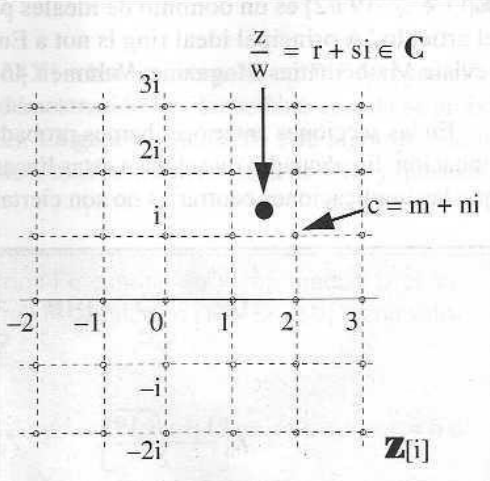
\includegraphics[scale=0.5]{./images/approximation.png}
	}
\end{figure}

\begin{example}[Resolución de ecuaciones lineales en los enteros de Gauss]
	Resolver la ecuación $2ix = 11i$ en $\mathbb{Z}[i]$ equivale a comprobar si $2i$ divide a $11i$. lo que en un dominio euclídeo implica ver que todo resto euclídeo es cero. Consideramos la fracción $\frac{11+7i}{2i}$ y la racionalizamos multiplicando denominador y numerador mediante $-2i$ obteniendo $\frac{-22i+14}{4} = \frac{-11i+7}{2}$ y por tanto $q = -6i+4$ y $r = (-6i+4)(11+7i) = -i+1$. El resto obtenido aquí es un resto euclídeo que no es cero. Por tanto, la ecuación no tiene solución. 
	
	En cambio, la ecuación $(7+2\sqrt{2})x = 4 + 7 \sqrt{2}$ tiene como única solución $x = \sqrt{2}$.
\end{example}


\pagebreak
\section{Dominios de ideales principales}
\subsection{Definición y propiedades fundamentales}

Existen caracterizaciones (véase Números, Grupos y Anillos, página 246) que aconsejan definir el siguiente concepto en el ambiente de los dominios de integridad. 

\begin{definition}[Dominio de ideales principales]
Dado un dominio de integridad $A$. 

$A$ es un dominio de ideales principales si todo ideal de $A$ es principal, esto es, $\forall I < A. \exists x \in A. I = \langle x \rangle$. 
\end{definition}

\begin{theorem}[Teorema de Bézout]
Dado un dominio de ideales principales $A$. 

1. $\forall a,b \in A \exists d=(a,b)$.\\
2. $\exists u,v \in A. d = au+bv$. 

A cualquier pareja $u,v$ que verifique la segunda ecuación se les llama coeficientes de Bézout. 
\end{theorem}
\begin{proof}
Dados $a,b \in A$, consideremos $\langle a,b \rangle = \{ax+by:x,y \in A\}$ este es el ideal generado por $a$ y $b$, esto es, el menor ideal que los contiene. En efecto, como $a,b \in \langle a,b \rangle$ sabemos que $\langle a,b \rangle$ no es vacío. También es claro que $\langle a,b \rangle$ es un ideal ya que $ax+by + ax' +by' = a(x+x')+b(y+y') \in I$ y $c(ax+by) = a(xc)+b(yc) \in I$. 

Utilizamos que $A$ es un dominio de ideales principales y obtenemos que debe existir $d \in A.\langle a,b \rangle = \langle d \rangle$ y por tanto $d = au+bv$ para convenientes $u,v \in A$. Por tanto, hemos deducido la segunda propiedad.

Por lo anterior, $d|a \land d|b$ y si $c \in A$ verifica que $c|a \land c|b$ entonces $c|au+bv$ de donde $c|d$. Esto nos dice que $d = (a,b)$
\end{proof}

\begin{example}[Un ejemplo de anillo de enteros cuadráticos que no es DIP]
Por los ejemplos anteriores como en $\mathbb{Z}[\sqrt{-5}]$ no existe el máximo común divisor de cualesquiera dos elementos tampoco puede ser un dominio de ideales principales. 
\end{example}

\begin{proposition}[Todo DE es un DIP]
Todo dominio euclídeo es un dominio de ideales principales donde cada ideal está generado por el elemento con valor mínimo de la función euclídea.  
\end{proposition}
\begin{proof}
Si $\phi$ es la función euclídea asociada al dominio y consideremos un ideal cualquiera $I \neq \{0\}$. El conjunto $\phi(I \setminus \{0\})$ es un subconjunto no vacío de números naturales y por tanto tiene mínimo. Sea $b$ este mínimo. Demostraremos que $I = \langle b \rangle$. 

$\subseteq)$ Dado que $b \in I \implies \langle b \rangle \subseteq I$. \\
$\supseteq)$ Dado $a \in I \setminus \{0\}$ tenemos que $\phi(a) \ge \phi(b)$. Por estar en un dominio euclídeo, $a = bq + r$ con $r = 0 \lor \phi(r) < \phi(b)$. Si $r = 0$ hemos acabado ya que entonces $a = bq \in \langle b \rangle$ y por tanto $I \subseteq \langle b \rangle$. Si $r \neq 0$ entonces necesariamente $\phi(r) < \phi(b)$. Pero esto contradice que $b$ sea el elemento de valor mínimo del conjunto anterior, ya que $r = a - bq \in I$ y $\phi(r) < \phi(b)$. 
\end{proof}

\begin{example}[Un DIP que no es DE]
$\mathbb{Z}[\frac{1+\sqrt{-19}}{2}]$ es un DIP pero no es DE.
\end{example}

\subsection{Retículo de divisibilidad y de ideales.}

\begin{corollary}[Existencia del mínimo común múltiplo en DIP]
En cualquier dominio de ideales principales (en particular, en los dominios euclídeos), existe el mínimo común múltiplo de cualquiera dos elementos.
\end{corollary}
\begin{proof}
En efecto, en un DIP por el teorema de Bézout existe el máximo común divisor de cualquier par de elementos y como un DIP es un dominio de integridad se tiene por la proposición anterior que existe el mínimo común múltiplo de cualquier par de elementos. 

Cualquier dominio euclídeo es un dominio de ideales principales. 
\end{proof}

\begin{corollary}[Retículo de divisibilidad]
Sea $D$ un dominio de ideales principales y sea $(,),[,]$ el máximo común divisor y el mínimo común múltiplo respectivamente. Entonces $(D,(,),[,])$ es un retículo.
\end{corollary}
\begin{proof}
Elijamos $[,]$ como ínfimo y $(,)$ como supremo. 

Por lo anterior, estas operaciones son internas en $D$. 

Claramente, se verifican las propiedades conmutativa, asociativa y la propiedad de idempotencia. Faltaría demostrar la propiedad de absorción que diría $[x,(x,y)] = x$ y $(x,[x,y]) = x$. 

Por otro lado, el máximo del retículo es el $1$ del dominio y el mínimo del retículo es el $0$ del dominio.

En consecuencia, $(a,1) = 1,(a,0) = a$. También el $0$ del dominio es el mínimo del retículo, y en particular, $[a,0] = 0,[x,1] = x$.
\end{proof}

\begin{tikzcd}
1    \\
x \arrow{u}{mcd} \arrow{d}{mcm}  \\   
0 
\end{tikzcd}


Pregunta: ¿este retículo es distributivo, es complementado? ¿Es el 1 el máximo y el 0 el mínimo o hay maximales (las unidades) y minimales? Aquí solo hace falta que sea distributivo y complementado para ser un álgebra de Boole. Ojo: quien es un retículo es $D/\sim$ donde $\sim$ es la relación de ser asociados. 

\begin{corollary}[Retículo de ideales de un DIP]
Sea $A$ un dominio de ideales principales consideremos el retículo de ideales ordenado por la inclusión las operaciones supremo e ínfimo y producto están definidas para este en términos del máximo común divisor y del mínimo común múltiplo. Más precisamente, para todo $a,b \in A$:

\begin{enumerate}
\item $\langle a \rangle + \langle b \rangle = \langle (a,b) \rangle$
\item $\langle a \rangle \cap \langle b \rangle = \langle [a,b] \rangle$
\item $\langle a \rangle \cdot \langle b \rangle = \langle ab \rangle$
\end{enumerate}
\end{corollary}
\begin{proof}
\begin{enumerate}
\item Es consecuencia del teorema de Bézout. 
\item Se deriva desde la definición. 
\item Se deriva desde la definición. 
\end{enumerate}
\end{proof}

\begin{proposition}[Ideales principales maximales son los generados por irreducibles]
Sea $A$ un dominio de ideales principales y $a \in A \setminus \{0\}$:

$\langle a \rangle$ es maximal $\iff a$ es irreducible.
\end{proposition}
\begin{proof}
$\Rightarrow)$ Si $\langle a \rangle$ es maximal y $a = bc$ entonces como todo ideal maximal es primo y $bc \in \langle a \rangle$ se tendría que $b \in \langle a \rangle \lor c \in \langle a \rangle$. Supongamos que $b \in \langle a \rangle$, entonces $b = ad = bcd$ y como $b \neq 0$ se simplifica a $1 = cd$ de modo que $c \in U(A)$ y la factorización es impropia de modo que $a$ es irreducible. 

$\Leftarrow)$ Supongamos que $a$ es irreducible y veamos que $\langle a \rangle$ es maximal. En efecto, como $a$ es irreducible, no es una unidad y por tanto, $\langle a \rangle \neq A$. Por otro lado, si $\langle a \rangle \subseteq \langle b \rangle \neq A$  entonces $b|a$ y $b \notin U(A), b \neq 0$, luego tenemos que $a = bc$ donde $c \neq 0$ y $c$ debe ser una unidad ya que no existen factorizaciones propias de $a$. Por tanto, $\langle a \rangle = \langle b \rangle$.
\end{proof}


\subsection{Solución de ecuaciones diofánticas y algoritmo de Euclides}

\begin{theorem}[Resolución de ecuaciones diofánticas lineales en un DIP]
Sea $A$ un dominio de ideales principales y $a,b,c \in A$ con $a,b \neq 0$. 

1. La ecuación diofántica lineal $ax+by = c$ tiene solución $\iff d|c$ con $d = (a,b)$. \\
2. Si $d|c$ y $(x_0,y_0)$ es una solución particular entonces la solución general da para cada $k \in A$ la solución $(x_0+k\frac{b}{d},y_0-k\frac{a}{d})$. 
\end{theorem}
\begin{proof}
\begin{enumerate}
\item La ecuación tiene solución $\iff c \in \langle a,b \rangle = \langle d \rangle \iff d|c$ con $d = (a,b)$. Donde hemos utilizado el corolario al teorema de Bézout.
\item Supongamos que $x_0,y_0$ es una solución particular. Claramente, para cada $k \in A$ la pareja $(x_0+k\frac{b}{d},y_0-k\frac{a}{d})$ es una solución particular ya que $a(x_0+k\frac{b}{d})+b(y_0-k\frac{a}{d}) = ax_0+by_0 = c$. 

Veamos que no hay más soluciones. Si $(x,y)$ es otra solución. Entonces restando las ecuaciones para $(x,y)$ y $(x_0,y_0)$ obtenemos $a(x-x_0)+b(y-y_0) = 0$, esto es, $a(x-x_0) = -b(y-y_0)$. Esto nos dice que $\frac{b}{d}$ divide a $\frac{a}{d}(x-x_0)$ y por el lema de Euclides como $(\frac{b}{d},\frac{a}{d}) = 1$ se verificará qque $\frac{b}{d}|(x-x_0)$. Por tanto, existe $k \in A$ tal que $x-x_0 = k\frac{b}{d}$ o equivalentemente $x = x_0 + k\frac{b}{d}$ como queríamos. Análogamente, existe un $h \in A$ tal que $y = y_0 - h \frac{a}{d}$. 

Pero resulta que $k = h$. Esto se puede ver sustituyendo en la ecuación $a(x-x_0)+b(y-y_0) = 0$ llegando a que $ab(k-h) = 0$. Dado que $a,b \neq 0$ y que $A$ es un dominio de integridad, $x = h$. 
\end{enumerate}
\end{proof}

El teorema anterior no da un método para calcular la solución particular $(x_0,y_0)$. 

Sabemos que $c = d \cdot c'$ por la condición de existencia de solución. Por otro lado, como $d = au+bv$ por la identidad de Bézout, tendríamos que $c = a(uc')+b(vc')$. Entonces elegimos $x_0 = uc' \land y_0 = vc'$. 

Es claro que en el anterior algoritmo necesitamos conocer $d,u,v$. El siguiente algoritmo, nos da los coeficientes de Bézout, el máximo común divisor y el mínimo común múltiplo. 

\begin{theorem}[Algoritmo extendido de Euclides]
Dado $A$ un dominio euclídeo y $a,b \in A$. 

\begin{enumerate}
\item Si $b = 0$ hemos acabado ya que $(a,0) = a$, $u = 1,v= 0$. 
\item Si $a = 0$ hemos acabado ya que $(0,b) = b$, $u = 0,v= 1$. 
\item Supongamos $a,b \neq 0$ y $\phi(a) \ge \phi(b)$. Si la desigualdad anterior no se da siempre podemos intercambiar $a$ y $b$ ya que $(a,b) = (b,a)$. 
\begin{itemize}
\item Dividir $a$ entre $b$ para obtener $a = bq_1+r_1$ con $r_1 = 0 \lor \phi(r_1) < \phi(b)$. 
\item Si $r_1 = 0 \implies (a,b) = b$.
\item Si $r_1 \neq 0 \implies (a,b) = (a-qb,b) = (b,r_1)$ . 
\end{itemize}
\item Análogamente se continúa obteniendo la lista de ecuaciones $$b = r_1q_2+r_2$$ $$r_1 = r_2q_3+r_3$$ $$\ldots$$ $$r_n = r_{n+1}q_{n+2}+r_{n+2}$$ Donde $r_{n+1} = 0$ y $r_n = (a,b) = (0,r_n)$. Se puede asegurar que llegaremos a este punto mediante el método de descenso infinito aplicado a la función euclídea de los restos. 

\item Para obtener los coeficientes de Bézout en cada paso se realiza el siguiente cálculo. 

Si $\alpha = au+bv$ y $\alpha' = au'+bv'$ entonces: $$\alpha'' = \alpha - \alpha'q = a(u-qu') + b(v-qv') = au'' + bv''$$ Finalmente, los coeficientes que se obtienen para $r_n$ son los coeficientes de Bézout para $a,b$ ya que $r_n = (a,b)$. De forma indirecta, $[a,b] = u_{n+1}a = v_{n+1}b$. 
\end{enumerate}

El procedimiento puede ser resumido en la siguiente tabla:

\begin{center}
  \begin{tabular}{ | l | c | r |}
    \hline
    $\alpha$ & u & v \\ \hline
    a & 1 & 0 \\ \hline
    b & 0 & 1 \\ \hline
    $r_1$ & $1$ & $-q_1$ \\ \hline
    $r_2$ & $-q_2$ & $1+q_1q_2$ \\ \hline
    $r_3$ & $1+q_1q_3$ & $-q_1-q_3-q_1q_2q_3$ \\ \hline
    $\cdots$ & $\cdots$ & $\cdots$ \\ \hline 
    $r_n$ & $u_n$ & $v_n$ \\ \hline
    $r_{n+1} = 0$ & $u_{n+1}$ & $v_{n+1}$ \\ 
    \hline
  \end{tabular}
\end{center}

Es importante darse cuenta como se obtienen los sucesivos coeficientes de Bézout en esta tabla. Se pasa de una fila a otra tomando las dos anteriores y restando a la última de ellas la anterior multiplicada por el cociente obtenido al dividir los correspondientes términos de la columna de la izquierda. 

Hacemos varias observaciones al método general. 

Primeramente es necesario observar que en cada paso, $r_i = a u_i + b v_i$ por construcción. 

La igualdad para el mínimo común múltiplo se deduce observando que la sucesión que hace las diferencias en cruz de productos de la primera fila y la segunda: $$w_i = u_i r_{i+1} - u_{i+1} r_i$$ es una sucesión constante que alterna el signo. En efecto: $$w_i = u_i r_{i+1} - s_{i+1} u_i = u_i (r_{i-1} - q_ir_i) - (u_{i-1} - q_i u_i) r_i = - (u_{i-1} r_i - u_i r_{i-1})$$ Como $w_0 = u_0 r_1 - u_1 r_0 = b$, se tendrá que $w_i = (-1)^i w_0$ y finalmente, para como $r_{n+1} = 0$, se tendría: $$w_{n+1} = (-1)^{n+1} b = - u_{n+1} mcd(a,b)$$ es decir: $$ab = (-1)^n u_{n+1} a (a,b)$$ Como estamos en un dominio de integridad, necesariamente, la ecuación tiene una única solución que es $[a,b] = u_{n+1}a$ donde recordamos que el mínimo común múltiplo es único salvo asociados. 
\end{theorem}

\begin{example}[Ejemplos de aplicación del algoritmo]
\begin{enumerate}
\item Aplicar el algoritmo de Euclides para $a = 30,b = 12$:

\begin{center}
  \begin{tabular}{ | l | c | r |}
    \hline
    $\alpha$ & u & v \\ \hline
    30 & 1 & 0 \\ \hline
    12 & 0 & 1 \\ \hline
    $6$ & $1$ & $-2$ \\ \hline
    $0$ & $-2$ & $5$ \\ \hline
  \end{tabular}
\end{center}

Como consecuencia, $(30,12) = 6$ y $[30,12] = -2 \cdot 30 = -60 \sim 60 = 5 \cdot 12$ y los coeficientes de Bézout son $1,-2$. 

\item Aplicar el algoritmo de Euclides para $a = 3+2i,b = 2-3i$:

Recordando cómo se divide en $\mathbb{Z}[i]$ tendríamos que:

\begin{center}
  \begin{tabular}{ | l | c | r |}
    \hline
    $\alpha$ & u & v \\ \hline
    $3+2i$ & 1 & 0 \\ \hline
    $2-3i$ & 0 & 1 \\ \hline
    $0$ & $1$ & $i$ \\ \hline
  \end{tabular}
\end{center}

Como consecuencia, $(3+2i,2-3i) = 2-3i$ y $[3+2i,2-3i] = 3+2i \cdot 1 = 3+2i = i \cdot 2-3i$ y los coeficientes de Bézout son $0,1$. 
\end{enumerate}
\end{example}


\pagebreak
\section{Congruencias}
\subsection{Ecuaciones en congruencias}

\begin{definition}[Relación de congruencia en dominios de integridad]
Sea A un dominio de integridad e $I \subseteq A$ un ideal. Definimos la relación $x,y \in A$ son congruentes modulo $I$ si $x-y \in I$. Lo notaremos $x \equiv_{I} y$.
\end{definition}

\begin{proposition}[Propiedades de las congruencias]\label{prop-congruencias}
Dado un dominio de integridad $A$. 

1. $\equiv_{I}$ es una relación de equivalencia sobre $A$. \\
2. $a \equiv_{I} b \implies ca \equiv_{I} cb$. (producto en ambos miembros) \\
3. $a \equiv_{I} b \iff a+c \equiv_{I} b+c$ (suma en ambos miembros)\\
4. $a \equiv_{I} b \land c \equiv_{I} d \implies a+c \equiv_{I} b+d$ (isotonía para la suma)\\
5. $a \equiv_{I} b \land c \equiv_{I} d \implies ac \equiv_{I} bd$ (isotonía para el producto)\\
6. $I = \{a \in A:a \equiv_{I} 0\}$ (caracterización del ideal)\\
\end{proposition}
\begin{proof}
1. $a \equiv_{I} a$ ya que $0$ siempre está en el ideal.\\
$a \equiv_{I} b \iff a-b \in I$ y como $I$ es cerrado para opuestos, $b-a \in I \iff b \equiv_{I} a$. \\
$a \equiv_{I} b \land b \equiv_{I} c \iff a-b \in I \land b-c \in I$, y como $I$ es cerrado para la suma $a-b+b-c = a-c \in I \iff a \equiv_{I} c$. 

2. $a \equiv_{I} b \iff a-b \in I$ y como $I$ es cerrado para múltiplos, dado $c \in A$, $c(a-b) \in I \iff ca \equiv_{I} cb$

3. $a \equiv_{I} b \iff a-b \in I \iff a+c-c-b \in I \iff a+c \equiv_{I} b+c$.

4. Por 3, $a \equiv_{I} b \implies a+c \equiv_{I} b+c \equiv_{I} b+d$.  

5. Por 2, $a \equiv_{I} b \implies ca \equiv_{I} cb \equiv_{I} bd$. 

6. $a \equiv_{I} 0 \iff a-0 \in I \iff  a \in I$.
\end{proof}

Para dar el recíproco de 2. tenemos que trabajar en una estructura más rica.  Nosotros vamos a centrarnos en la hipótesis de dominio de ideales principales. Podemos modificar la notación. Ya que todo ideal $I$ es principal, existe $m \in A$ tal que $I = \langle m \rangle$. Y tendremos: $$a \equiv b \; mod(m) \iff a-b \in \langle m \rangle \iff m | a-b \iff \exists q \in A. a = mq+b$$ donde las equivalencias son válidas en cualquier dominio de integridad. 

\begin{proposition}[Simplificación del factor común]
	Dado A un dominio de ideales principales. 
	
	$ca \equiv_{m} cb \land (c,m) = 1 \implies a \equiv_{m} b$.
\end{proposition}
\begin{proof}
	De la congruencia deducimos que $m|c(a-b)$ y como $(c,m) = 1$, por el lema de Euclides, sabemos que $m|a-b$ o equivalentemente $a \equiv_{m} b$. 
\end{proof}

Los ejemplos prácticos serán dominios euclídeos. 

\begin{proposition}[Caracterización de la relación de congruencia en dominios euclídeos]
Dado un dominio euclídeo con unicidad de cocientes y restos ($\mathbb{Z}, K[X]$).

$a \equiv b \; mod(m) \iff$ a y b dan el mismo resto al dividirlos por m.

\end{proposition}
\begin{proof}
$\Rightarrow)$ Por ser $A$ un dominio euclídeo sabemos que $a = qm+r$ con $r = 0 \lor \phi(r) < \phi(m)$. Tratemos de hallar a partir de esta descomposición, la descomposición euclídea para $b$ apoyándonos en que $a,b$ son congruentes. Por la congruencia sabemos que $b = a + pm$. Podemos entonces escribir $b = a + pm = qm + r + pm = m(p+q)+r$ y esta es la descomposición euclídea de $b$ ya que $r = 0 \lor \phi(r) < \phi(m)$ por hipótesis. 

$\Leftarrow)$ Supongamos que $a = qm+r \land b = q'm+r$ con $r = 0 \lor \phi(r) < \phi(m)$. Para ver que son congruentes restamos estas ecuaciones y obtenemos: $$a-b = (q-q')m \in \langle m \rangle \iff a \equiv b \; mod(m)$$
\end{proof}

Tratamos ahora el problema de resolver $ax \equiv b \; mod(m)$. Esta es una ecuación lineal entendida en el anillo cociente $\frac{A}{\langle m \rangle}$. En efecto: $$ax \equiv b \; mod(m) \iff ax-b \in \langle m \rangle \iff (a+\langle m \rangle)(x+\langle m \rangle) = (b+\langle m \rangle)$$ Damos a continuación el método general para resolverlas:

\begin{theorem}[Resolución de congruencias lineales]
Sea $A$ un dominio de ideales principales. \\
Sean $a,m \neq 0$ (en otro caso la ecuación degenera a una igualdad o a la no ecuación). \\
Notemos $d=(a,m)$.

1. La ecuación $ax \equiv b \, (mod \, m)$ tiene solución si y sólo si $d | b$.\\
2. Si la ecuación tiene solución, la ecuación es equivalente a $\frac{a}{d}x \equiv \frac{b}{d} \, (mod \, \frac{m}{d})$.\\
3. Como $(\frac{a}{d},\frac{m}{d}) = 1$ existe $u,v \in A$ tales que $1 = \frac{a}{d}u+\frac{m}{d}v$ y por tanto $x_0 = u\frac{b}{d}$ es una solución particular de la ecuación $\frac{a}{d}x \equiv \frac{b}{d} \, (mod \, \frac{m}{d})$.\\
4. Si $x_0$ es una solución particular, la solución general se obtiene como $x = x_0 + k \frac{m}{d}$ donde $k \in A$. Dicho de otro modo la ecuación de partida equivale a la ecuación $x \equiv x_0 \, (mod \, \frac{m}{d})$.\\
5. Si A es un dominio euclídeo, podemos garantizar que existe una solución particular $x_1$ de $ax \equiv b \; mod(m)$ tal que $x_1 = 0 \lor \phi(x_1) < \phi(\frac{m}{d})$. Dicho de otro modo, la ecuación es equivalente a $x \equiv x_1 mod \; \Big(\frac{m}{d}\Big)$ y $x = x_1 + k\frac{m}{d}$ es la solución general óptima. 
\end{theorem}
\begin{proof}
1. La ecuación $ax \equiv b \; mod(m)$ tiene solución si y sólo si: $$\exists x. m | b-ax \iff \exists x,y. b-ax = my \iff \exists x,y.ax+my = b \iff d = (a,m) | b$$ por la existencia de soluciones para la ecuación diofántica lineal. 

2. Comprobamos que tienen las mismas soluciones. x es solución de $ax \equiv b mod(m)$ si y sólo si: $$m|ax-b \iff d\frac{m}{d}\Big|d\Big(\frac{a}{d}x-\frac{b}{d}\Big) \iff \frac{m}{d} \Big| \frac{a}{d}x-\frac{b}{d}$$ luego x es solución de $\frac{a}{d}x \equiv \frac{b}{d} mod(\frac{m}{d})$. Obsérvese que en la simplificación hemos utilizado que $d \neq 0$ ya que $a \neq 0 \land d|a$.

3. Dado que $(\frac{a}{d},\frac{m}{d})$ y que $A$ es un dominio de ideales principales, por el teorema de Bézout se tiene que $\exists u,v \in A. 1 = \frac{a}{d}u+\frac{m}{d}v$. Podemos multiplicar esta expresión obteniendo $\frac{b}{d} = \frac{b}{d}\frac{a}{d}u + \frac{b}{d}\frac{m}{d}v$. Claramente entonces $x_0 = \frac{b}{d}u$ es una solución particular de $\frac{a}{d}x \equiv \frac{b}{d} mod(\frac{m}{d})$. 

4. Dada una solución particular de la ecuación original, también lo será de la ecuación $\frac{a}{d}x \equiv \frac{b}{d} mod(\frac{m}{d})$. Podemos utilizar entonces la regla de simplificación del factor común ya que $A$ es un dominio de ideales principales de modo que si $x$ es otra solución de la ecuación se tendría $\frac{a}{d}x \equiv \frac{a}{d}x_0 mod(\frac{m}{d})$ y como $(\frac{a}{d},\frac{m}{d}) = 1$ podemos simplificarlo a $x \equiv x_0 mod(\frac{m}{d})$.

Recíprocamente, toda solución de esta forma verificará $\frac{a}{d}x_0 \equiv \frac{b}{d} mod(\frac{m}{d}) \land x \equiv x_0 mod(\frac{m}{d})$ y por tanto $\frac{a}{d}x \equiv \frac{a}{d}x_0 \equiv \frac{b}{d} mod(\frac{m}{d})$ y sabemos que esta ecuación es equivalente a la original.

5. Una vez llegados a la ecuación $x \equiv x_0 \; mod(\frac{m}{d})$ podemos dividir $x_0$ entre $\frac{m}{d}$ obteniendo $x_0 = \frac{m}{d}q + x_1$ con $x_1 = 0 \lor \phi(x_1) < \phi(\frac{m}{d})$.  Está claro que $x_0 \equiv x_1 \; mod(\frac{m}{d})$ de modo que la ecuación $x \equiv x_1 \; mod(\frac{m}{d})$ es equivalente a $x \equiv x_0 \; mod(\frac{m}{d})$ y hemos obtenido una solución general óptima. 
\end{proof}

Podemos realizar la siguiente observación al método general que permite simplificar las operaciones:

\begin{proposition}[Simplificación del factor común en la forma reducida]
Sea $A$ un dominio de ideales principales.

Dada la ecuación $ax \equiv b \; mod(m)$ la transformamos en su equivalente $\frac{a}{d}x \equiv \frac{b}{d} \; mod(\frac{m}{d})$ con $d = (a,b)$. Supongamos que $c$ es un divisor común de $\frac{a}{d}$ y $\frac{b}{d}$. Entonces la ecuación es equivalente a $\frac{\frac{a}{d}}{c}x \equiv \frac{\frac{b}{d}}{c} \; mod(\frac{m}{d})$. 
\end{proposition}
\begin{proof}
La demostración es evidente por la propiedad de simplificación del factor en dominios de ideales principales. En efecto, como $(\frac{a}{d}, \frac{m}{d}) = 1$, si $c|\frac{a}{d} \land c| \frac{b}{d}$ entonces $d' = (c,\frac{m}{d}) = 1$. Supóngase que $d' \nsim 1$ (el máximo común divisor es único salvo asociados) entonces $d'|c|\frac{a}{d} \implies d'|\frac{a}{d} \land d'|\frac{m}{d}$ y por tanto $d'|d = 1 \implies d' \sim 1$.   
\end{proof}

\begin{example}
\begin{itemize}
\item En $\mathbb{Z}$ consideramos la ecuación $60x \equiv 90 \; mod(105)$. 

Calculamos $d = (60,105) = 15(4,7) = 15$. Como $15|90$ la ecuación tiene solución y es equivalente a $4x \equiv 6 \; mod(7)$. La observación permite simplificar aún más hasta $2x \cong 3 \; mod(7)$. 

Para resolver la ecuación calculamos mediante el algoritmo extendido de Euclides, los coeficientes de Bézout y la descomposición $(2,7) = 1 = 2 \cdot 4 + 7 \cdot (-1)$. Tomamos módulo 7 en ambos miembros y obtenemos $2 \cdot 4 \equiv 1 \; mod(7)$. Finalmente, multiplicamos la expresión por el término independiente de la ecuación obteniendo $2 \cdot 12 \equiv 3 \; mod(7)$. La solución particular obtenida es $x_0 = 12$. La solución general sería $x = 12 + k \cdot 7$ con $k \in \mathbb{Z}$.

Dado que $\mathbb{Z}$ es un dominio euclídeo podemos obtener una solución óptima dividiendo $x_0$ entre 7. El resultado es $12 = 7 \cdot 1 + 5$. La solución general óptima sería $x = 5 + 7 \cdot k$ con $k \in \mathbb{Z}$.

\item También se puede simplificar antes de transformar el sistema. Por ejemplo si tenemos la ecuación $1100x \equiv 660 \; mod(140)$ podemos dividir por $140$, obteniendo el sistema $120x \equiv 100 \; mod(140)$. 

Calculamos $d = (120,140) = 20(6,7) = 20$ y obtenemos el sistema equivalente $6x \equiv 5 \; mod(7)$ que podemos resolver directamente multiplicando por $6$ ya que $6^{-1} = 6$, obteniendo $x \equiv 2 \; mod(7)$ que ya está en su forma general óptima. 
\end{itemize}
\end{example}

\subsection{Sistemas de congruencias}

Dado un dominio de ideales principales $A$ nos planteamos la solución general del sistema de congruencias lineales dado por:

\[   
\begin{cases}
a_1x \equiv b_1 \; mod(m_1) \\
a_2x \equiv b_2 \; mod(m_2) 
\end{cases}
\]

Una solución de este sistema es una solución de cada una individualmente. Por tanto, podemos simplificar a estudiar el sistema en forma resuelta:

\[   
\begin{cases}
x \equiv a \; mod(m) \\
x \equiv b \; mod(n) 
\end{cases}
\]

\begin{theorem}[Resolución de un sistema de congruencias lineales en forma resuelta]
Consideremos un dominio de ideales principales $A$. Considérese el sistema: 

\[   
\begin{cases}
x \equiv a \; mod(m) \\
x \equiv b \; mod(n) 
\end{cases}
\]

1. El sistema tiene solución $\iff a \equiv b \; mod((m,n))$ (teorema chino de los restos). \\
2. Si $x_0$ es una solución particular entonces la solución general es $x = x_0 +k[m,n]$ donde $k \in A$.\\
3. Si $A$ es un dominio euclídeo, podemos garantizar que existe una solución particular $x_1$ tal que $x_1 = 0 \lor \phi(x_1) < \phi([m,n])$. Dicho de otro modo, la ecuación es equivalente a $x \equiv x_1 \; mod([m,n])$ y $x = x_1 + k [m,n]$ es la solución general óptima. 
\end{theorem}
\begin{proof}
Obsérvese que como $A$ es un dominio de ideales principales siempre existen el máximo común divisor y el mínimo común múltiplo de cualesquiera dos elementos. 

1. Claramente, las soluciones de la primera ecuación son de la forma $x = a +km$ con $k \in A$. Veamos qué forma, tienen que tener estas soluciones para satisfacer la segunda ecuación. Tendría que verificar $a+km \equiv b \; mod(n) \iff mk \equiv b-a \; mod(n)$. Esta ecuación tiene solución si y sólo si: $$(m,n)|b-a \iff \exists p \in A. b-a = p(m,n) \iff a \equiv b \; mod((m,n))$$

2. Supongamos que $k_0$ es una solución particular de la ecuación $mk \equiv b-a \; mod(n)$, entonces la solución general daría para cada $t \in A$, la solución $k = k_0 + t \frac{n}{(m,n)}$ y la solución general al sistema original sería $x = a + (k_0 + t \frac{n}{(m,n)})m = (a+k_0m)+ t \frac{nm}{(n,m)} = (a+k_0m)+t[m,n]$. Entonces identificamos $x_0 = a+k_0m$ como solución particular y por tanto la solución general es como la dada en el enunciado. 

3. En el caso en que $A$ sea un dominio euclídeo la solución general $x \equiv x_0 \; mod([m,n])$ se puede convertir en óptima dividiendo $x_0$ por $[m,n]$ de donde se obtiene $x \equiv x_1 \; mod([m,n])$ y $x_1$ reúne las condiciones del enunciado. 
\end{proof}

Podemos realizar la siguiente observación al método general que permite simplificar las operaciones:

\begin{proposition}[Solución con módulos primos relativos]
Supongamos el siguiente sistema:

\[   
\begin{cases}
x \equiv a \; mod(m) \\
x \equiv b \; mod(n) 
\end{cases}
\]

donde $(m,n) = 1$. Si la descomposición de Bézout es de la forma $1 = mu + nv$ entonces $x_0 = bmu + anv$ es una solución particular y $x \equiv x_0 \; mod(mn)$ es la solución general del sistema. 
\end{proposition}
\begin{proof}
En efecto, claramente $x_0 \equiv_{m} anv$ y tomando módulos en la expresión de Bézout se tiene que $x_0 \equiv a \; mod(m)$. Por tanto, $x_0 \equiv_{m} a$. Análogamente, se tiene que $x_0 \equiv_{n} b$. Por tanto, $x_0$ es una solución particular del sistema. 

La solución general es de la forma $x = x_0 + k[m,n]$ con $k \in A$ y como $(m,n) = 1$, se tiene que $mn = [m,n]$ y por tanto la solución general es de la forma $x = x_0 + kmn$. 
\end{proof}

\begin{example}
Supongamos que tenemos que resolver el sistema:

\[   
\begin{cases}
6x \equiv 8 \; mod(11) \\
5x \equiv 15 \; mod(23) 
\end{cases}
\]

lo primero ponerlas en forma resuelta mediante el procedimiento indicado en la solución de una ecuación lineal. Sin embargo, en vez de utilizar Bézout podemos observar que en la primera ecuación el inverso de 6 es 2 y en la segunda ecuación que dado que $(5,23) = 1$ podemos dividir el factor y el término independiente por 5 resultando el siguiente sistema:

\[   
\begin{cases}
x \equiv 5 \; mod(11) \\
x \equiv 3 \; mod(23) 
\end{cases}
\]

El procedimiento para hallar una solución particular del sistema consiste en sustituir la solución general de la primera ecuación en la segunda ecuación y resolver para esta. Así, la solución general de la primera es $x = 5+11t$ y al sustituir queda: $$5+11t \equiv 3 \; mod(23)$$ $$11t \equiv -2 \; mod(23)$$ En esta última  ecuación observamos que podemos multiplica por $2$ obteniendo $$-t \equiv -4 \; mod(23)$$ $$t \equiv 4 \; mod(23)$$ Por tanto $t_0 = 4$ es una solución particular de esta ecuación y la solución particular del sistema será $x_0 = 5+11 \cdot 4 = 49$ de modo que la solución general es $x \equiv 49 \; mod(253)$. 

\end{example}

Una generalización de la proposición nos proporciona el siguiente algoritmo:

\begin{proposition}[Algoritmo de Lagrange]
Dado un sistema de congruencias lineales en forma resuelta de la forma $x \equiv a_i \; mod(m_i)$ supongamos que $\forall j \neq k. (m_j,m_k) = 1$. 

Sea $c_k = \frac{\prod m_i}{m_k}$ entonces se verifica que $(m_k,c_k) = 1$ y por el teorema de Bézout existen $u_k,v_k$ tales que $u_kc_k+v_km_k = 1$ y observamos que $x_k = u_kc_k \equiv 1 \; mod(m_k)$. 

Observamos que $a = \sum a_ix_i$ es una solución particular del sistema de modo que la solución general del sistema viene dada por $x \equiv a \; mod(\prod m_i)$. 
\end{proposition}

\subsection{Anillo de restos de un dominio euclídeo con unicidad de cocientes y restos}

\begin{definition}[Módulo válido]
Sea $A$ un dominio euclídeo con unicidad de cocientes y restos.

Diremos que $m \in A \setminus \{0\}$ es un módulo válido si $m \notin U(A)$ y además $\phi(1) < \phi(m)$ donde $\phi$ es la función euclídea considerada. 
\end{definition}

En los ejemplos usuales, $\mathbb{Z},K[X]$ la condición anterior no es restrictiva ya que $\phi(1) < \phi(m)$ para todo elemento no nulo, no unidad. En particular, considerar módulos válidos garantiza que el resto de la división de $1$ por el módulo $m$ es precisamente $1$, lo cual será importante para relacionar el conjunto de restos con el anillo cociente. 

\begin{definition}[Anillo de restos]
Dado $A$ un dominio euclídeo con unicidad de cocientes y restos y $m \in A$ un módulo válido. 

Denotamos por $A_m$ el conjunto de todos los restos que se obtienen al dividir los elementos del anillo entre $m$. Si $R_m(a)$ es el resto de dividir $a$ entre $m$ entonces tenemos que: $$A_m = \{R_m(a):a \in A\} \subseteq A$$ Este conjunto puede dotarse con estructura de anillo con las operaciones $$a+b = R_m(a+b) \text{ y } ab = R_m(ab)$$ Se le llama el anillo de restos módulo $m$.  
\end{definition}

\begin{proposition}[Estructura cociente del anillo de restos]
Se $A$ un dominio euclídeo con unicidad de cocientes y restos y $m \in A$ un módulo válido. 

\begin{enumerate}
\item $(A_m,+,\cdot)$ es un anillo.
\item $(A_m,+,\cdot)$ no es, en general, un subanillo en de $A$.
\item $A_m \cong A/mA$
\end{enumerate}
\end{proposition}
\begin{proof}
\begin{enumerate}
\item Las propiedades de anillo se derivan de las de $A$. Observemos que al haber asegurado que $\phi(1) < \phi(m)$ tenemos que $0 \neq 1$ son dos elementos del anillo y distintos, ya que, $0 = m0+0$ y $1 = m0 + 1$. 

\item $A_m$ no es en general un subanillo. Por ejemplo, $\mathbb{Z}_n$ es un anillo que no es subanillo de $\mathbb{Z}$ ya que no contiene a $-1$. 

\item La aplicación $R_m:A \to A_m$ tal que $a \mapsto R_m(a)$ es un epimorfismo de anillos. En este punto, es crucial utilizar la unicidad de cocientes y restos. Por ejemplo, para demostrar que $R_m(a+b) = R_m(R_m(a)+R_m(b))$ (nótese que la operación de la derecha es la de $A_m$), expresaríamos: $$a+b = mq_1 + r_1, a = mq_2+r_2, b = mq_3 +r_3$$ de donde: $$a+b = m(q_2+q_3) + mq_4 + r_4 = m(q_1+q_2+q_3)+r_4$$ donde $r_4$ se ha elegido para que verifique las condiciones de la división euclídea. Análogamente, se procede para la multiplicación. Además, $R_m(1) = 1$ se garantiza, ya que $1 = m0+1$ con $\phi(1) < \phi(m)$ de modo que $1$ es un resto válido (en el caso de los enteros, al ser positivo también tiene que ser el único). El núcleo es $\langle m \rangle$ y por el primer teorema de isomorfía tenemos que $\frac{A}{\langle m \rangle} \cong A_m$. 
\end{enumerate}
\end{proof}

\begin{example}[Dos formas de mirar al anillo de restos]
El anillo $\mathbb{Q}[X]_{X^2+X+1} = \{aX+b:a,b \in \mathbb{Q}\}$ es isomorfo al anillo $\mathbb{Q}[X]/\langle X^2+X+1 \rangle$ donde trabajaríamos con clases de congruencias. 
\end{example}

Vamos a estudiar cuales de entre estos anillos de restos son cuerpos y como se resuelven las ecuaciones en congruencias en este caso particular. 

\begin{proposition}[Resolución de ecuaciones en congruencias en anillos de restos]
Sea $A$ un dominio euclídeo con unicidad de cocientes y restos y $n$ un módulo válido.

1. Dados $a,b \in A_n$ con $a \neq 0$, $ax = b$ en $A_n$ tiene solución $\iff d = (a,n)|b$.\\
2. En el caso de $\mathbb{Z}_n$ la ecuación tiene exactamente $d$ soluciones que partiendo de la solución inicial $x_0$ con $x_0 = 0 \lor \phi(x_0) < \phi(\frac{n}{d})$ son $\{x_0+k\frac{n}{d}:k = 0,\cdots,d-1\}$. 
\end{proposition}
\begin{proof}
1. Dados $a,b \in A_n \setminus \{0\}$ queremos resolver la ecuación $ax = b$, esta ecuación tiene una solución $x$ cuando: $$ax = b \iff [ax] = [b] \iff ax \equiv b \; mod(n) \iff (a,n)|b$$ 

2. En tal caso sabemos por el teorema de resolución de una congruencia lineal que existe una solución particular en $\mathbb{Z}$ con $x_0 = 0 \lor \phi(x_0) < \phi(\frac{n}{d})$ y que las soluciones son de la forma $x = x_0 + k\frac{n}{d}$ con $k \in \mathbb{Z}$. 

Dado que $\mathbb{Z}_n \equiv \frac{\mathbb{Z}}{<n>}$ el problema es equivalente a resolver la ecuación $[a][x] = [b]$ con incógnita $[x]$. La solución general es $\{[x_0+k\frac{n}{d}]: k \in \mathbb{Z}\}$. 

Las clases $[x_0 + k \frac{n}{d}]$ con $k = 0,\cdots,d-1$ son todas distintas. En efecto, si $0 \le k' < k < d$ entonces: $$0 < \Big(x_0 + k\frac{n}{d}\Big) - \Big(x_0+k'\frac{n}{d}\Big) = (k-k')\frac{n}{d} < d \frac{n}{d} = n$$ de donde $x_0 + k \frac{n}{d} < x_0 + k \frac{n}{d}$ y por tanto todos estos elementos son distintos lo que implica que sus clases también los son. 

Veamos que no hay más clases distintas. Dado $k \in \mathbb{Z}$ tomamos la división euclídea de $k$ entre $d$, esto es, $k = qd+r$ con $r = 0 \lor \phi(r) < \phi(d)$. Entonces $$x = x_0 + k \frac{n}{d} = x_0 + \Big(qd \frac{n}{d}\Big) + r \frac{n}{d} \equiv_{\frac{n}{d}} x_0 + r\frac{n}{d}$$ donde $r = 0 \lor \phi(r) < \phi(d)$ y por tanto el elemento estaría entre las anteriores. 

Volviendo al anillo de restos $\mathbb{Z}_n$ tenemos que los representantes anteriores coinciden con sus restos ya que $x_0 + k \frac{n}{d} < \frac{n}{d} + (d-1) \frac{n}{d} = n$. 
\end{proof}

\begin{example}[Ecuación lineal en los enteros módulo 105]
Resolver la ecuación $60x = 90$ en $\mathbb{Z}_{105}$.

Pasamos la ecuación al anillo cociente como $60x \equiv 90 \; mod(105)$. Como $(60,105)=15(4,7) = 15$ y $\frac{90}{15} = 6$, la ecuación tiene soluciones. Resolvemos la congruencia por el método habitual obteniendo la ecuación equivalente $4x \equiv 6 \; mod(7)$ en la que podemos utilizar la propiedad de simplificación en dominios de ideales principales para obtener la ecuación $2x \equiv 3 \; mod(7)$. Aquí es fácil ver que una solución particular es $x_0 = 5$ de modo que el conjunto de soluciones será $\{5+k7:k=0,\cdots,14\}$. 
\end{example}

Habíamos visto que en cualquier anillo se tenían tres familias bien diferenciadas, las unidades, los divisores de cero y el resto de elementos. En un anillo de restos estas familias quedan reducidas a dos:

\begin{proposition}[Partición por unidades y divisores de cero del anillo de restos]
Sea $A$ un dominio euclídeo con unicidad de cocientes y restos y $m$ un módulo válido. Denotamos por $(,)$ al máximo común divisor en $A$. Entonces:

1. $U(A_m) = \{a \in A_m \setminus \{0\}:(a,m) = 1\}$.\\
2. Las unidades y los divisores de cero forman una partición de $A_m$. Esto es, $A_m = U(A_m) \dot\cup 0_{A_m}$.  
\end{proposition}
\begin{proof}
1. $a \in U(A_m) \iff \exists x. ax = 1 \iff (a,m)|1 \iff (a,m) = 1$.

2. Ya vimos en las propiedades de los divisores de cero que $U(A) \cap 0_A = \emptyset$. 

Veamos que $A_m = U(A_m) \cup 0_{A_m}$. 

Tomemos $a \in A_m \setminus U(A_m)$ y veamos que $a \in 0_{A_m}$.  Como $a$ no es unidad, $d = (a,m) \neq 1$.

Veamos que $[\frac{m}{d}] \neq [0]$ razonado por reducción al absurdo: $$\Big[\frac{m}{d}\Big] = [0] \implies \exists x. \frac{m}{d} = xm \implies m = xmd \implies 1 = xd \implies d \in U(A)$$ donde la ecuación se resuelve en el dominio de integridad $A$ y llegamos a una contradicción con la elección de $a$. 

En consecuencia, $[a][\frac{m}{d}] = [a \cdot \frac{m}{d}] = [\frac{a}{d}m] = [0]$ y como los divisores de cero son invariantes por isomorfismo y $A_m \cong \frac{A}{\langle m \rangle}$ se tiene que también $a \in A_m$ es un divisor de cero.
\end{proof}

\begin{example}[Unidades en anillos de restos]
1. $U(\mathbb{Z}_n) = \{0 \le a < n:(a,n) = 1\}$. \\
2. Claramente, si $[a] \in \frac{A}{mA} \setminus \{0\}$ entonces $[a] \in U(\frac{A}{mA}) \iff (a,m) = 1$.  
\end{example}

El siguiente teorema puede deducirse de la teoría de dominios de ideales principales y de la de ideales maximales y primos. Aquí lo hacemos con las herramientas desarrolladas hasta ahora:

\begin{theorem}[Caracterización de los anillos de restos de módulo irreducible]
Dado un anillo de restos $A_m$. 

$m$ es irreducible $\iff A_m$ es un dominio de integridad $\iff A_m$ es un cuerpo.
\end{theorem}
\begin{proof}
$3 \implies 2)$ Trivial. 

$2 \implies 3)$ Como $A_m$ es un dominio de integridad, tenemos que $0_{A_m} = \{0\}$. Por lo anterior, $A_m = U(A_m) \dot\cup 0_{A_m} = U(A_m) \dot\cup \{0\}$. Por tanto, $A_m$ ha de ser un cuerpo. 

$1 \implies 3)$ Sea $[a] \in \frac{A}{\langle m \rangle} \setminus \{[0]\}$ entonces $m \nmid a$ y como $m$ es irreducible se tiene que $(a,m) = 1$, esto nos dice que $a \in U(A_m)$ pero como las unidades son invariantes por isomorfismo también $[a] \in U(\frac{A}{\langle m \rangle})$. De modo que $\frac{A}{\langle m \rangle}$ es un cuerpo. 

$2 \implies 1)$ Lo hacemos por contrarrecíproco. Si $m$ no es irreducible entonces $m$ se puede descomponer como $m = ab$ con $a,b \notin U(A_m) \cup A(m)$. 

Teniendo en cuenta que $a,b$ son los únicos restos de una división euclídea entre $m$, no pueden ser múltiplos de $m$ ya que en otro caso aumentaríamos el cociente de la división y tomaríamos resto $0$. Pero $a,b$ no pueden ser $0$ ya que en este caso $m = 0$ no sería irreducible. En consecuencia, $[a],[b] \neq [0]$ en $\frac{A}{\langle m \rangle}$. 

Sin embargo, $[a][b] = [ab] = [m] = [0]$, esto es, $[a],[b]$ son divisores de cero en $\frac{A}{\langle m \rangle}$ y como los divisores de cero son invariantes por isomorfismo, se tiene que $a,b$ serían divisores de cero y por tanto $A_m$ no sería un dominio de integridad. 
\end{proof}

\begin{corollary}[Anillos de restos que son cuerpos]
1. $\mathbb{Z}_n$ es un cuerpo $\iff$ $n$ es irreducible. \\
2. $K[X]_{f(x)}$ es un cuerpo $\iff f(x)$ es irreducible en $K[X]$.\\
2. Si $n,f(x)$ no son irreducibles entonces $\mathbb{Z}_n,K[X]_{f(x)}$ no son dominios de integridad. 
\end{corollary}

\begin{example}[Cuerpos finitos]
Por lo anterior, $\mathbb{Z}_p[X]$ con $p$ primo es un dominio euclídeo y $\mathbb{Z}_p[X]_{q(x)}$ con $q$ irreducible es un cuerpo. Este cuerpo, tiene un número finito de elementos de la forma: $$p(x) = a_{n-1}x^{n-1}+ \cdots + a_0$$ esto da un total de $p^n$ elementos. Se puede demostrar que estos son los únicos cuerpos finitos que hay. 
\end{example}


\begin{theorem}[Teorema chino de los restos revisitado]
Dado un dominio euclídeo $A$ con unicidad de cocientes y restos y $m,n \in A \setminus \{0\}$. 

$(m,n) = 1 \iff A_{mn} \cong A_m \times A_n$. 

La aplicación que los hace isomorfismo es $a \mapsto (R_n(a),R_m(a))$ y su inversa se computa como en la proposición sobre la solución de un sistema de congruencias con módulos que son primos relativos.
\end{theorem}
\begin{proof}
$\Rightarrow)$ Consideremos el esquema siguiente:

\begin{tikzcd}
A \arrow{r}{p} \arrow{d}[swap]{p'} &
\frac{A}{<n>} \times \frac{A}{<m>}  \\   
\frac{A}{<mn>} \arrow[swap]{r}{\cong} & 
Img(p) \arrow{u}{i}
\end{tikzcd}

La aplicación proyección $p(a) = ([a]_n,[a]_m)$ es un homomorfismo de anillos cuyo núcleo está formado por aquellos elementos que son múltiplos de $m$ y de $n$, esto es $Ker(p) = \langle [m,n] \rangle$ y ya que $(m,n) = 1$ se tiene que $Ker(p) = \langle mn \rangle$. 

Veamos que es epimorfismo, esto es, dadas dos clases $[b]_n,[c]_m$ existe $x \in A$ tal que $[x] = [b] = [c]$. Esto es equivalente a resolver el siguiente sistema de ecuaciones:

\[   
\begin{cases}
x \equiv b \; mod(n) \\
x \equiv c \; mod(m) 
\end{cases}
\]

Por el teorema chino de los restos, el sistema solución sólo cuando $b \equiv c \; mod((m,n))$ y como en este caso, $(m,n) = 1$ es claro, que el sistema tiene solución.

Entonces, por el primer teorema de isomorfía se tiene que $\frac{A}{<mn>} \cong \frac{A}{<n>} \times \frac{A}{<m>}$ con el isomorfismo dado por $[a]_{mn} = ([a]_n,[a]_m)$. 

En conclusión se tiene el isomorfismo deseado: $$A_{mn} \cong A_n \times A_m$$ dado por $a \mapsto (R_n(a),R_m(a))$. 

$\Leftarrow)$ Si asumimos un isomorfismo $A_{mn} \cong A_m \times A_n$ entonces cualquier sistema de ecuaciones de la forma:

\[   
\begin{cases}
x \equiv a \; mod(n) \\
x \equiv b \; mod(m) 
\end{cases}
\]

tiene solución. Si elegimos $a = 1$ y $b = 0$ la condición de que el sistema tenga compatibilidad implica que $1 \equiv 0 \; mod((m,n))$ pero entonces $1 \in \langle (m,n) \rangle$  y en consecuencia, $(m,n)$ es una unidad. Pero el máximo común divisor es único salvo asociado luego podemos considerar que $(m,n) = 1$.
\end{proof}

\begin{example}[Un ejemplo en el que no es válido el teorema chino]
Observemos que $\mathbb{Z}_4 \ncong \mathbb{Z}_2 \times \mathbb{Z}_2$ pues $(2,2) = 2$. Además $\mathbb{Z}_4$ tiene 2 unidades mientras que $\mathbb{Z}_2 \times \mathbb{Z}_2$ tiene solo una. 
\end{example}

\subsection{Consecuencias en el anillo $\mathbb{Z}_n$}

\begin{definition}[Función $\phi$ de Euler]
La función $\phi$ de Euler es la función $\phi:\mathbb{N}-\{0,1\}$ tal que $\phi(n) = |U(\mathbb{Z}_n)|$, esto es, para cada $n$ da la cantidad de números menores que $n$ y primos con $n$. 
\end{definition}

\begin{proposition}[Propiedades para el cálculo de la función de Euler]
	Se verifican las siguientes propiedades:
\begin{enumerate}
	\item Si $p \in \mathbb{N}$ es primo y $e \ge 1$ entonces $\phi(p^e) = p^{e} - p^{e-1} = p^{e}(1- \frac{1}{p})$
	\item Si $m,n \in \mathbb{N}$ y $(m,n) = 1$ entonces $\phi(mn) = \phi(m)\phi(n)$.
\end{enumerate}
\end{proposition}
\begin{proof}
\begin{enumerate}
	\item Tenemos que $\phi(p) = U(\mathbb{Z}_{p^e}) = \{a:(a,m) = 1\}$ y por tanto, del conjunto $\{1,2,3,\cdots,p^e\}$ tenemos que quitar los múltiplos de $p$ que son $\{1p,2p,\cdots,p^{e-1}p\}$, es decir, $p^{e-1}$ elementos.
	\item Por el teorema de los restos, como $(m,n)$ tenemos que $\mathbb{Z}_{mn} \cong \mathbb{Z}_m \times \mathbb{Z}_n$ y como las unidades se preservan por isomorfismo y las unidades del producto son exactamente el producto de unidades de cada factor se tiene que: $$\mathbb{Z}_{mn} \cong \mathbb{Z}_m \times \mathbb{Z}_n$$ $$U(\mathbb{Z}_{mn}) \cong U(\mathbb{Z}_m) \times U(\mathbb{Z}_n)$$ Por tanto, se tendrá: $$\phi(mn) = |U(\mathbb{Z}_{mn})| = |U(\mathbb{Z}_n)||U(\mathbb{Z}_m)| = \phi(n)\phi(m)$$ 
\end{enumerate}

\end{proof}

\begin{theorem}[Teorema de Euler para el cálculo de $\phi$]
Sea $n = \prod_{i = 1}^r p_i^{e_r}$ con $p_i$ irreducibles distintos de $\mathbb{Z}$. Entonces:

$\phi(n) = n(1 - \frac{1}{p_1}) \cdots (1-\frac{1}{p_r})$
\end{theorem}
\begin{proof}
Dado $n \in \mathbb{N}$ de la forma del enunciado usando el segundo apartado de la proposición anterior tenemos que $$\phi(n) = \prod \phi(p_i^{e_i}) = \prod p_i^{e_i}\Big(1- \frac{1}{p_i}\Big) = n \prod \Big(1- \frac{1}{p_i}\Big)$$ Obsérvese que $\phi$ no depende de los eponentes de la descomposición en irreducibles. 	
\end{proof}

\begin{example}
	$\phi(36) = 36(1-1/3)(1-1/2) = 12$ y por tanto en $\mathbb{Z}_{36}$ hay exactamente 24 divisores de cero y exactamente 12 unidades. 
\end{example}

Para establecer el siguiente resultado necesitamos el lema siguiente:

\begin{lemma}[Lema de Lagrange]
Sea $G$ un grupo finito conmutativo con $m$ elementos. Entonces $\forall a \in G. a^m = 1$. 
\end{lemma}
\begin{proof}
Fijado $a \in G$, la aplicación $l:G \to G$ tal que $x \mapsto ax$ es una aplicación biyectiva ya que si $ax = ay \implies a^{-1}ax = a^{-1}ay \implies x = y$ por tanto es inyectiva y es sobreyectiva ya que para $y \in G$ si elijo $x = a^{-1}y \implies y = ax$. Nótese la siguiente igualdad: $$s = \prod_{x \in G} x = \prod_{x \in G} (ax) = a^m \prod_{x \in G} x = a^ms \implies a^m = 1$$
\end{proof}

\begin{theorem}[Teorema de Euler]
	Sea $n \ge 2$. 
	
	\begin{enumerate}
		\item Si $a \in \mathbb{Z} \land (a,n) = 1$ entonces $a^{\phi(n)} \equiv 1 \; mod(n)$ 
		\item Si $a \in \mathbb{Z}_n \land (a,n) = 1$ entonces $a^{\phi(n)} = 1$ en $\mathbb{Z}_n$ en particular $a^{-1} = a^{\phi(n) - 1}$
	\end{enumerate}
\end{theorem}
\begin{proof}
Aplicamos el lema anterior al grupo de las unidades de $\mathbb{Z}_n$ que tiene $\phi(n)$. 

Si $(a,n) = 1 \implies a \in U(\mathbb{Z}_n) \implies a^{\phi(n)} = 1$ en $\mathbb{Z}_n$. 

Tomando clases de equivalencia, se tendrá que $[a]^{\phi(n)} = [1]$ o equivalentemente $a^{\phi(n)} \equiv 1 \; mod(n)$. 
\end{proof}

\begin{corollary}[Teorema pequeño de Fermat]
	Sea $p \ge 0$ un irreducible de $\mathbb{Z}$.
	
	\begin{itemize}
		\item Si $a \in \mathbb{Z} \land p \nmid a$ entonces $a^{p-1} \equiv 1 \; mod(p)$ 
		\item Si $a \in \mathbb{Z}_p \land a \neq 0$ entonces $a^{p-1} = 1$ en $\mathbb{Z}_p$ en particular $a^{-1} = a^{p-2}$
	\end{itemize}
\end{corollary}
\begin{proof}
Basta tener en cuenta que $U(\mathbb{Z}_p) = \mathbb{Z}_p \setminus \{0\}$ y en particular tiene $p-1$ elementos. 
\end{proof}

\begin{example}
	Calcular $10^{47^{51}}$ en $\mathbb{Z}_{14}$. 
	
	Las herramientas para resolver este tipo de problemas son las propiedades de las congruencias y la función de Euler. 
	
	Por un lado, $10^{47^{51}} = 5^{47^{51}} 2^{47^{51}}$. 
	
	Centrándonos en el primer factor, como $(5,14) = 1$ podemos aplicar el teorema de Euler, esto es: $$5^{\phi(14)} \equiv 5^6 \equiv 1 \; mod(14) \implies 5^{6q+r} \equiv 5^r \; mod(14)$$ Entonces podemos dedicarnos a resolver $47^{51} \equiv 5^{51} \; mod(6)$. Por el teorema de Euler, observando que $(5,6) = 1$ tenemos que: $$5^{\phi(6)} \equiv 5^2 \equiv 1 \; mod(6) \implies 5^{2q+r} \equiv 5^r \; mod(6)$$  y como $51 \equiv 1 \; mod(2)$ entonces $47^{51} \equiv 5 \; mod(6) \implies 5^{47^{51}} \equiv 5^5 \equiv 3 \; mod(14)$.
	
	Centrándonos en el segundo factor, como $(2,14) = 2$ no podemos usar el teorema de Euler y sólo nos quedan las herramientas de congruencias. Observando que $2^4 \equiv 2 \; mod(14)$ tenemos que para todo $k$: $$2^{3k} \equiv 8 \; mod(14)$$ $$2^{3k+1} \equiv 2 \; mod(14)$$ $$2^{3k+2} \equiv 4 \; mod(14)$$ y bastaría estudiar el exponente módulo 3: $$47^{51} \equiv 2^{51}  \equiv 2 \; mod(3)$$ Donde el último paso se debe a observar que $2^3 \equiv 2 \; mod(3)$. Por tanto, $2^{47^{51}} \equiv 4 \; mod(14)$. 
	
	Finalmente, $10^{47^{51}} \equiv 3 \cdot 4 \equiv 12 \; mod(14)$.
\end{example}

\begin{example}
	Calcular $3^{81}$ en $\mathbb{Z}_{100}$. 
	
	Este ejercicio ilustra una tercera herramienta que puede ser útil cuando falla lo anterior. Estamos hablando del teorema chino de los restos. En esta situación los cálculos directos requieren el uso de calculadora y el teorema de Euler nos dice que $3^{90} \equiv 1 \; mod(100)$, lo que no contribuye a resolver la situación. Por tanto, veamos cómo usamos el teorema chino de los restos. 
	
	Para estudiar $3^{81}$ en $\mathbb{Z}_{100}$ puedo estudiar $3^{81}$ en $\mathbb{Z}_4$ y $\mathbb{Z}_{25}$. Por el teorema de Euler, en estos casos $3^{81} = 3$ y claramente esto implica que $3^{81} = 3$ en $\mathbb{Z}_{100}$. Si no fuera tan directo bastaría expresar la combinación de Bézout $1 = 4(-1) + 5\cdot 1$ y poner la solución particular $x_0 = 3 \cdot 4 \cdot (-1) + 5 \cdot 3 \cdot 1 = 3$. 
\end{example}

\begin{lemma}[Raíces cuadradas de la unidad en $\mathbb{Z}_p$]
Sea $p$ un número primo. 

Las raíces cuadradas de la $1 \in \mathbb{Z}_p$ son exactamente $1$ y $-1$. 
\end{lemma}
\begin{proof}
Claramente, $1,-1$ son raíces. Por otro lado, como $\mathbb{Z}_p$ es un dominio de integridad si $a$ fuera una raíz cuadrada de la unidad entonces: $$0 = (a^2-1) = (a-1)(a+1)$$ Si $a-1$ y $a+1$ fueran no nulos entonces llegamos a una contradicción por tanto $a = -1$ o $a = 1$. 
\end{proof}

El siguiente teorema se aprovecha de la interpretación de las raíces cuadradas de la unidad como aquellos elementos que coinciden con su inverso. 

\begin{theorem}[Teorema de Wilson]
Sea $p$ un entero positivo. 

$p$ es primo $\iff (p-1)! \equiv -1 \; mod(p)$.
\end{theorem}
\begin{proof}
$\Rightarrow)$ El hecho de que las raíces cuadradas de la unidad en $\mathbb{Z}_p$ con $p$ primo sean $1,-1$ implica que sólo $1,-1$ son inversos multiplicativos de sí mismos. Todos las demás unidades tendrán como inverso un elemento distinto. Por tanto, $$(p-1)! = \prod_{i = 1}^{p-1} i = 1 \cdot \Big(\prod_{i = 2}^{p-2} i\Big) \cdot (p-1) = -\prod_{j \in \mathbb{Z}_p \setminus \{1,p-1\}} jj^{-1} = -1$$

$\Leftarrow)$ En $\mathbb{Z}_p$ tenemos la ecuación $(p-1)! = -1$ luego en $\mathbb{Z}$ tenemos que $$(p-1)! + 1 = pq \implies pq - (p-1)! = 1 \implies (p,(p-1)!) = 1$$ donde hemos utilizado que $\mathbb{Z}$ es un dominio de ideales principales. Pero entonces no hay ningún número menor que $p$ que divida a $p$. Esto es, $p$ es primo. 
\end{proof}







\pagebreak
\section{Dominios de factorización única}
\subsection{Definición y expresión de los elementos del dominio}

\begin{definition}[Dominio de factorización única]
Sea $A$ un dominio de integridad tal que:

1. Para todo el elemento $a \in A$ no nulo ni unidad, existe una factorización $a = \prod_{i = 1}^{r} p_i$ irreducibles. \\
2. La factorización es única salvo el orden y la relación de asociados, esto es, si $a = \prod_{i = 1}^r p_i = \prod_{i = 1}^s q_i$ con $p_i,q_i$ irreducibles entonces $r = s$ y $\exists \sigma \in S_r$ tal que $\forall i \in \{1,\cdots,r\}.p_i \sim q_{\sigma(i)}$ 
\end{definition}

\begin{example}[Primeros ejemplos de DFU]
Los siguientes son ejemplos sencillos de DFU:

\begin{enumerate}
\item $\mathbb{Z}$ es un DFU por el teorema fundamental de la aritmética. 
\item Cualquier cuerpo es un DFU ya que todo elemento es nulo o unidad y por tanto, la definición de DFU es vacía en este caso. 
\item $\mathbb{Z}[\sqrt{-5}]$ no es un DFU ya que $6 = 23 = (1+\sqrt{-5})(1+\sqrt{-5})$ serían dos factorizaciones en irreducibles no asociados entre sí. 
\end{enumerate}
\end{example}

Recordemos que la irreducibilidad se mantiene por la relación de asociados. En particular, las clases de equivalencia para esta relación estarán formadas en su totalidad por elementos irreducibles o por el contrario no contendrán ningún elemento irreducible. Entonces, seleccionamos las clases formadas sólo por irreducibles y tomamos un representante de cada clase. Formamos entonces un conjunto $\mathcal{P}$ tal que todo elemento de $\mathcal{P}$ es irreducible, todo irreducible de $A$ está asociado con uno de $\mathcal{P}$ y donde es claro que en $\mathcal{P}$ no hay asociados. 

\begin{example}
\begin{itemize}
\item En $\mathbb{Z}$ la clase $\mathcal{P}$ podría ser la de los números primos positivos.
\item En $K[X]$ con $K$ un cuerpo puedo tomar los polinomios con coeficiente líder uno ya que la relación ser asociado se traduce en este dominio euclídeo por la relación diferenciarse en una constante. 
\end{itemize}
\end{example}

El siguiente teorema da la unicidad salvo el orden de la descomposición. 

\begin{theorem}[Teorema fundamental de la aritmética para DFU]
Sea $A$ un DFU y $a \in A$ no nulo ni unidad y  $\mathcal{P}$ una colección de representantes de los irreducibles por la relación de asociados.  

$\exists u \in U(A),p_i \in \mathcal{P}$ con $p_i \neq p_j$ y $e_i \ge 1$ tales que $a = u \prod_{i = 1}^n p_i^{e_i}$ (existencia de la descomposición)

Además si, $a = v \prod_{i = 1}^m q_i^{f_i}$ con $v \in U(A)$, $q_i \in \mathcal{P}$ con $q_i \neq q_j$ y $f_i \ge 1$ entonces $u = v, n = m$ y $\exists \sigma \in S_n. p_i = q_{\sigma(i)} \land e_i = f_{\sigma(i)}$ (unicidad salvo el orden de los factores)  
\end{theorem}
\begin{proof}
Veamos la existencia de la descomposición:

Por ser $A$ un DFU tenemos que $a = \prod_{i = 1}^r p_i$ con $p_i$ irreducibles. Estos $p_i$ estarán asociados con los correspondientes representantes de su clase de equivalencia en $\mathcal{P}$, esto es, $p_i = u_i p_i'$ con $p_i' \in \mathcal{P}$ y por tanto $a = \prod_{i = 1}^r u_i \prod_{i = 1}^r p_i'$ y podemos asumir que los $p_i'$ son todos distintos ya que en caso contrario los agrupamos en potencias. Como $u = \prod_{i = 1}^r u_i \in U(A)$ obtenemos finalmente una factorización $a = u \prod_{i = 1}^n p_i'^{e_i}$ con $e_i \ge 1$, $p_i' \neq p_j'$ y $p_i' \in \mathcal{P}$. 

Veamos ahora que la factorización es única salvo permutación de factores. Por inducción:

Escribimos $a = u \prod_{i = 1}^n p_i'^{e_i} = v \prod_{i = 1}^m q_i^{f_m}$. 

Si $n = 0$ entonces $a = u = v \prod_{i = 1}^m q_i^{f_m}$ claramente por la conmutatividad se tiene que los $q_i^{f_i} \in U(A)$ luego como $f_i \ge 1$ se tendrá necesariamente que $q_i \in U(A)$ en contradicción con que $q_i$ es un elemento irreducible. Por tanto, debe ser $m = 0$ y resulta $u = v$. 

Si $n > 0$ entonces $a = u \prod_{i = 1}^n p_i'^{e_i} = v \prod_{i = 1}^m q_i^{f_m}$. Ahora, $p_1$ debe estar asociado con algún $q_i$ por definición de DFU y como en $\mathcal{P}$ no hay asociados, se deduce que $p_1 = q_i$. Tras una reordenación de los factores podemos garantizar que $p_1 = q_1$. 

Discutamos ahora qué ocurre si $e_1 < f_1$. Nos queda entonces que $p_1^{e_1}(u \prod_{i = 2}^n p_i^{e_i}) = p_1^{e_1}(vp_1^{f_1-e_1}  \prod_{i = 2}^n q_i^{f_i})$ y como estamos en un dominio de integridad se obtiene $u \prod_{i = 2}^n p_i^{e_i} = v p_1^{f_1-e_1} \prod_{i = 2}^n q_i^{f_i}$. Como cada $q_i$ está asociado a un $p_i$ salvo el $p_1$ que por la elección de $\mathcal{P}$ no puede estar asociado con ninguno, esta ecuación se puede ver como $a = p_1^{t_1} (au)$ de modo que si $t_1 > 0$ deduciríamos que $p_1$ sería una unidad, en contradicción con que es un irreducible. Por tanto, $e_1 = f_1$ y nos queda que $u \prod_{i = 2}^n p_i^{e_i} = v \prod_{i = 2}^m q_i^{f_i}$. 

Finalmente, por hipótesis de inducción, $n = m$ y $\exists \sigma \in S_{n-1}$ tal que $p_i = q_{\sigma(i)} \land e_i = f_{\sigma(i)}$. La composición de las dos permutaciones obtenidas nos da la composición necesaria para la demostración del teorema. 
\end{proof}

\begin{definition}[Expresión canónica de un elemento en un DFU]
Dado $p \in \mathcal{P},a \in A \setminus \{0\}$. Si $a = u\prod_{i = 1}^r p_i^{r_i}$ entonces denotamos $u(a) = u$ y $e(p_i,a) = e_i$ para los irreducibles de la factorización y $e(p,a) = 0$ para los irreducibles que no aparecen en la factorización. De modo que para cualquier $a \in A \setminus \{0\}$ podemos escribir: $$a = u(a) \prod_{p \in \mathcal{P}} p^{e(p,a)}$$ aunque $\mathcal{P}$ puede ser infinito, este producto está reducido a un conjunto finito de ellos y esta expresión tiene la ventaja de ser única y sugiere cómo con los irreducibles se pueden generar todos los elementos como si fueran los ladrillos de construcción de los elementos del dominio. 
\end{definition}

\subsection{Relación de divisibilidad en un DFU}

\begin{proposition}[Divisibilidad en un DFU]
Dado un DFU $A$ y $\mathcal{P}$ una colección de representantes de los irreducibles por la relación de asociados.

\begin{enumerate}
\item $a|c \iff \forall p \in \mathcal{P}. e(p,a) \le e(p,c)$
\item $\forall a,b \in A. (a,b) = \prod_{p \in \mathcal{P}} p^{min(e(p,a),e(p,b))}$
\item $\forall a,b \in A. [a,b] = \prod_{p \in \mathcal{P}} p^{max(e(p,a),e(p,b))}$
\end{enumerate}
\end{proposition}
\begin{proof}
\begin{enumerate}
\item Como $a|c$, $\exists b.c = ab$ y por tanto $$c = u(c) \prod_{p \in \mathcal{P}} p^{e(p,c)} = u(a) \prod_{p \in \mathcal{P}} p^{e(p,a)} u(b) \prod_{p \in \mathcal{P}} p^{e(p,b)} = u(a)u(b) \prod_{p \in \mathcal{P}} p^{e(p,a)+e(p,b)}$$ De aquí, tenemos que $u(c) = u(a) \cdot u(b)$ y $\forall p \in \mathcal{P}.e(p,c) = e(p,a) + e(p,b) \le e(p,a)$. 

Recíprocamente, basta tomar $$b = u(c)u(a)^{-1} \prod_{p \in \mathcal{P}} p^{e(p,c)-e(p,a)}$$ donde observamos que por hipótesis $e(p,c)-e(p,a) \ge 0$. En este caso: $$ba = \Big[u(c)u(a)^{-1} \prod_{p \in \mathcal{P}} e^{e(p,c)-e(p,a)}\Big] \cdot \Big[u(a) \prod_{p \in \mathcal{P}} p^{e(p,a)}\Big] = u(c)\prod_{p \in \mathcal{P}} p^{e(p,c)} = c$$
\item Se utiliza la caracterización anterior. 
\item Se utiliza la caracterización anterior teniendo en cuenta que hemos demostrado que como existe el máximo común divisor de cualesquiera dos elementos también existe el mínimo común múltiplo de cualesquiera dos elementos. 
\end{enumerate}
\end{proof}

\begin{proposition}[Relación entre primos e irreducibles en DFU]
Sea $A$ un DFU y $p \in A$ entonces $p$ es irreducible 
$ \iff p$ es primo. 
\end{proposition}
\begin{proof}
En cualquier dominio de integridad se verifica que si $p$ es primo entonces es irreducible. Veamos la otra implicación. 

Sea $p$ es un irreducible de $A$ con $A$ un DFU. Supongamos que $p|ab$ entonces por la relación de divisibilidad en DFU sabemos que $$e(p,ab) \ge e(p,p) = 1$$ y claramente $$e(p,ab) = e(p,a) + e(p,b)$$ Entonces necesariamente será $e(p,a) > 0 \lor e(p,b) > 0$ en cuyo caso $p|a \lor p|b$ y por tanto, $p$ es primo. 
\end{proof}

\subsection{Caracterizaciones alternativas}

\begin{theorem}[Caracterización de los DFU]
Sea $A$ un dominio de integridad. 

$A$ es DFU sí y sólo si se cumplen alguno de los siguientes pares de condiciones:

\begin{itemize}
\item Todo elemento no nulo ni unidad es producto de irreducibles. 
\item Todo irreducible es primo.
\end{itemize}

O bien:

\begin{itemize}
\item Todo elemento no nulo ni unidad es producto de irreducibles.
\item $\forall a,b \in A. \exists (a,b)$. 
\end{itemize}
\end{theorem}
\begin{proof}
\begin{itemize}
\item $\Leftarrow)$ Supongamos que $x \in A$ es un elemento no nulo y no unidad. Entonces, por hipótesis, $x = \prod_{i = 1}^r p_i = \prod_{j = 1}^s q_j$ donde $p_i,q_j$ son irreducibles. 

Queremos ver que $r = s \land \exists \sigma \in S_r.p_i \sim q_{\sigma(i)}$. Procedemos por inducción sobre $r$:

\begin{itemize}
\item Si $r = 1$, entonces si suponemos $s > 1$ tendríamos que $x = p = q_1 \ldots q_s$ de donde por la primera igualdad, $x$ es irreducible. Como $A$ es un DFU tendremos que $x$ es primo. Entonces como $x|q_1 \ldots q_s$ entonces $x |q_i$ y como $q_i|x$ entonces $x \sim q_i$, esto es, $x = uq_i = q_1 \ldots q_s$ con $u \in U(A)$ de donde como $A$ es un dominio de integridad, $\prod_{j \neq i} q_j = u$. Esto implica que $\forall i \neq j.q_j \in U(A)$ en contradicción con que son irreducibles. Por tanto, $r = s$ y $x = p = q_1$.

\item Si $r > 1$ y $x = \prod_i p_i = \prod_j q_j$ entonces dado que $p_1$ sería irreducible y por tanto primo, como antes, vemos que $p_1 \sim q_j$ y salvo una reordenación podemos suponer que $j = 1$. 

En este punto, queda $\prod_i p_i = \prod_j q_j \implies \prod_{i = 2}^r p_i = u \prod_{j = 2}^s q_j$ de modo que podemos aplicar la hipótesis de inducción obteniendo salvo reordenaciones que $p_i \sim q_j$ y que $r = s$. Como queríamos demostrar. 
\end{itemize}

$\Rightarrow)$ La primera parte se sigue de la definición de DFU. La segunda parte, es consecuencia de la proposición anterior.

\item $\Leftarrow)$ Vamos a ver que todo irreducible es primo. Sea $p$ irreducible y supongamos que $p|bc$. Distinguimos casos:

\begin{itemize}
\item Si $p|b$ hemos acabado. 
\item Si $p \nmid b$ entonces como por hipótesis existe $(p,b)$ y como $p$ es irreducible entonces $(p,b) = 1$.

En efecto, como $(b,p)|p$ que es irreducible, entonces $(b,p)$ es una unidad o un asociado a $p$. Si $(b,p)$ es unidad entonces $(b,p) = 1$ y hemos acabado. Si $(b,p) \in A(p)$ entonces $(b,p) = up$ con $u \in U(A)$ y por la unicidad del máximo común divisor salvo asociados, $(b,p) = p$. Por definición $(b,p) = p | b$ pero por hipótesis, $p \nmid b$. Contradicción.  

Finalmente, por el lema de Euclides, $p|c$. 
\end{itemize}

$\Rightarrow)$ Hemos demostrado anteriormente que en un DFU, $\forall a,b. (a,b) = \prod_{p \in \mathcal{P}} p^{min(e(p,a),e(p,b))}$. 

\end{itemize}
\end{proof}

\begin{corollary}[Existencia de mcd garantiza que los irreducibles son primos]
Sea $A$ un dominio de integridad tal que $\forall a,b \in A. \exists (a,b)$. Entonces:

$p$ es primo $\iff p$ es irreducible.
\end{corollary}
\begin{proof}
Siempre se da en un dominio de integridad que todo elemento primo es irreducible. En la prueba anterior, hemos mostrado que bajo la hipótesis de existencia del máximo común divisor, todo irreducible es primo.
\end{proof}

\subsection{Los DIP son DFU}

Sumamos a nuestros ejemplos de DFU a todos los DIP y DE. 

\begin{definition}[Anillo noetheriano]
Un anillo $A$ es noetheriano si para toda cadena de ideales $I_1 \subseteq I_2 \subseteq \cdots \subseteq I_n \subseteq \cdots$ se verifica que $\exists m. \forall k \ge 0. I_m = I_{m+k}$. 
\end{definition}

\begin{lemma}[Los DIP son anillos noetherianos]
Todo DIP es un anillo noetheriano.
\end{lemma}
\begin{proof}
Si $A$ es un DIP y consideramos una cadena ascendente de ideales $I_k \subseteq A$, podemos considerar su unión $U = \cup_{n \mathbb{N}} I_n$. Esta unión es un ideal. En efecto, si $x,y \in U$ entonces $\exists m,n. x \in I_n \land y \in I_m$. Supongamos sin pérdida de generalidad que $n < m$. Como la cadena es ascendente, $x+y \in I_m \subseteq U$. Si tomamos $x \in U, a \in A$, entonces $\exists n. x \in I_n$ y como $I_n$ es un ideal claramente $xa \in I_n \subseteq U$. 

Utilizando que $A$ es un DIP, $\cup_{n \in \mathbb{N}} I_n = \langle a \rangle$ para $a \in A$. Claramente, habrá un primer ideal $I_m$ que contiene a $a$ y desde $I_m$ la cadena ya no puede crecer, esto es, $I_{m+k} \subseteq I_m$. Matemáticamente, $a \in I_m \implies \langle a \rangle \subseteq I_m \implies \cup_{n \in \mathbb{N}} I_n = I_m \implies \forall k \ge 0. I_{m+k} \subseteq I_m$ y la otra inclusión se tiene por hipótesis. 
\end{proof}

\begin{theorem}[Los DIP son DFU]
Todo DIP es un DFU. 
\end{theorem}
\begin{proof}
Sea $A$ un DIP. Sabemos que existe el máximo común divisor de cualesquiera dos elementos y por tanto, tenemos la propiedad 2. de la caracterización alternativa de DFU. Veamos que se verifica que todo elemento $x \neq 0 \land x \notin U(A)$ es producto de irreducibles. Procedemos en dos pasos:

\begin{enumerate}
\item $a$ tiene un factor irreducibles. 

Si $a_0 = a$ es irreducible hemos acabado. En otro caso, debe admitir una factorización propia $a = a_1c_1$. Como $a_1|a$, $\langle a \rangle \subset \langle a_1 \rangle$ con inclusión estricta ya que si $\langle a \rangle = \langle a_1 \rangle$ entonces $a_1 \sim a$ y la factorización sería impropia. 

Continuando este proceso obtendríamos una cadena de ideales con $\langle a_i \rangle \subset \langle a_{i+1} \rangle$ para todo $i \ge 0$. Como $A$ es noetheriano, esta cadena debe estacionar en un $\langle a_r \rangle$. Este $a_r$ tiene que ser irreducible (su ideal resulta maximal) ya que en otro caso el procedimiento daría ideales mayores. 

Por tanto, $a = \prod_{i = 1}^r a_i$ con $a_r$ irreducible. 

\item $a$ es producto de un número finito de irreducibles. 

Repetimos el razonamiento anterior, si $c_0 = a$ no es irreducible entonces existe una factorización propia $a = p_1c_1$ con $p_1$ irreducible. Repitiendo el proceso en $c_i$ se obtiene una cadena con $\langle c_i \rangle \subset \langle c_{i+1} \rangle$ para todo $i \ge 0$. De nuevo, se observa que la cadena es de inclusiones estrictas, ya que en otro caso $c_i \sim c_{i+1}$ y la factorización sería impropia. 

Esta cadena debe estacionar en un $\langle c_{r} \rangle$ que resultará ser irreducible ya que en otro caso el procedimiento continúa la cadena. En conclusión, $a = p_1 \ldots p_r c_r$ con $p_i,c_r$ irreducibles. 
\end{enumerate}
\end{proof}










\pagebreak
\section{Anillos de polinomios sobre un DFU}
\subsection{Anillos de polinomios sobre un cuerpo}

Merece la pena comentar el caso en que $K[X]$ con $K$ un cuerpo. Dado que $K[X]$ es un dominio euclídeo también es un DFU. Estudiamos la factorización de polinomios de $K[X]$.

\begin{definition}[Cuerpo algebraicamente cerrado]
Un cuerpo $K$ es algebraicamente cerrado si todo polinomio no constante de $K[X]$ tiene raíz en $K$.
\end{definition}

\begin{example}[Los números complejos son algebraicamente cerrados]
El primer ejemplo lo proporciona el conjunto $\mathbb{C}$ de los números complejos. El teorema fundamental del álgebra garantiza que en $\mathbb{C}[X]$ todo polinomio no constante factoriza como producto de polinomios lineales, lo cual, es una definición equivalente a que $\mathbb{C}$ sea algebraicamente cerrado. 
\end{example}

\begin{proposition}[Unidades e irreducibles en los anillos de polinomios sobre un cuerpo]
Se verifican las siguientes propiedades:

\begin{enumerate}
\item Las unidades de $K[X]$ son los polinomios constantes no nulos.
\item Los polinomios de grado 1 son irreducibles en $K[X]$. Estos son los únicos irreducibles si y sólo si $K$ es algebraicamente cerrado.
\end{enumerate}
\end{proposition}
\begin{proof}
\begin{enumerate}
\item Si $q \in U(K[X])$ entonces $q$ tiene que ser de grado $0$ ya que por ser un dominio de integradad $0 = gr(1) = gr(qq^{-1}) = gr(q) + gr(q^{-1}) \ge gr(q)$ y si $gr(q) > 0$ se llega a una contradicción. Dado que $q$ es una unidad, no puede ser nulo. 

Recíprocamente, un polinomio constante no nulo, es una unidad, ya que $K$ es un cuerpo.  
\item Veamos que los polinomios lineales son irreducibles. Como $K$ es un cuerpo, un polinomio lineal sólo puede tener un factor de como mucho grado $1$. Por tanto, toda descomposición es una constante por un factor de grado $1$. Pero las constantes son unidades y por tanto, un factor es una unidad y el otro es asociado al polinomio de partida. Por tanto, el polinomio es irreducible. 

Si $K$ es algebraicamente cerrado todo polinomio descompone en lineales y por tanto no puede haber irreducibles de otro grado. Recíprocamente, si no hay irreducibles de otro grado, los polinomios descomponen y esto se ve como el cuerpo es algebraicamente cerrado. 
\end{enumerate}
\end{proof}

\begin{example}[Polinomios irreducibles con coeficientes complejos]
Los polinomios irreducibles en $\mathbb{C}[X]$ son exactamente los de grado 1. Por ejemplo, el polinomio $X^2+1$ es irreducible sobre $\mathbb{R}$ ya que no tiene raíces en $\mathbb{R}$ y sin embargo en $\mathbb{C}$ es reducible ya que $X^2+1 = (X-i)(X+i)$. 
\end{example}


\subsection{Anillos de polinomios sobre un DFU.}

\begin{definition}[Contenido de un polinomio. Polinomios primitivos.]
Sea $A$ un DFU.

Dado $f = \sum_{n \ge 0} a_if_i \in A[X]$ con $gr(f) \ge 1$, el contenido de $f$ es $$c(f) = (a_0,\cdots,a_n) \in A$$ el máximo cómun divisor de los coeficientes de $f$. El contenido de un polinomio es único salvo asociados. 

Si $c(f) = 1$ decimos que $f$ es primitivo. 
\end{definition}

\begin{lemma}[Herramientas auxiliares al lema de Gauss]
Dado $A$ un DFU y consideremos que los polinomios implicados a tienen grado mayor o igual que $1$. 

Si $f \in A[X]$ entonces:

1. $\forall a \in A. c(af) = ac(f)$. \\
2. $f = c(f)f'$ con $f'$ primitivo.

Sea $K = Q(A)$ el cuerpo de fracciones de $A$ e identifiquemos $A[X]$ como subanillo de $K[X]$. 

3. Dado $\phi \in K[X]$ podemos escribir $\phi = \frac{a}{b}f$ con $f \in A[X]$ primitivo y $a,b \in A$.\\
4. Todo polinomio en $K[X]$ es asociado con un polinomio primitivo de $A[X]$. 

Por tanto, el conjunto de representantes de las clases de asociación irreducibles en $K[X]$ puede elegirse en el conjunto de los polinomios primitivos de $A[X]$.
\end{lemma}
\begin{proof}
1. Basta extender por inducción al caso finito, la propiedad de linealidad del máximo común divisor: $$(ac,bc) = (a,b)c$$

2. Basta sacar factor común el contenido del polinomio como $f = c(f)f'$ y aplicando la propiedad anterior nos damos cuenta que $c(f) = c(c(f)f') = c(f)c(f')$. Como $A$ es un dominio de integridad, se tendrá alguna de las siguientes posibilidades:

\begin{itemize}
\item $c(f) = 0$ en cuyo caso el polinomio es nulo. Pero $gr(f) \ge 1$. Contradicción. 
\item $c(f') = 1$ por la propiedad de simplificación en dominios de integridad.
\end{itemize} 

3. Sea $\phi = \sum_{i \ge 0} \frac{a_i}{b_i} X^i$ y $b = \prod b_i$ entonces $b\phi = \sum_{i \ge 0} \frac{b}{b_i}a_iX^i \in A[X]$ y por el apartado anterior, $b\phi = af$ con $f \in A[X]$ primitivo. Por tanto, $\phi = \frac{a}{b}f$ es la expresión buscada. 

4. Dado $\phi \in K[X]$, por lo anterior, podemos expresarlo como $\phi = \frac{a}{b}f$ con $f$ primitivo y ya que $\frac{a}{b} \in U(K)$, deducimos que $\phi \sim f$.  
\end{proof}

\begin{lemma}[Lema de Gauss]
Sea $A$ un DFU y sean $f,g \in A[X]$ con $gr(f),gr(g) \ge 1$.

\begin{enumerate}
\item Si $f,g$ son primitivos entonces $fg$ es primitivo.
\item Equivalentemente, $c(fg) = c(f)c(g)$. 
\end{enumerate}
\end{lemma}
\begin{proof}
\begin{enumerate}
\item Sea $f = \sum_{i \ge 0} a_iX^i$ y $g = \sum_{j \ge 0} b_jX^j$ y notemos $fg = \sum_{k \ge 0} c_k X^k$. Por tanto, la expresión de los $c_k$ es $c_k = \sum_{i+ j = k} a_ib_j$. Queremos probar que $1 = (c_o, \ldots, c_k)$. 

Por reducción al absurdo supongamos que $1 \neq (c_o, \ldots, c_k)$. Como el contenido no es nulo (ya que entonces $fg = 0$ y $f,g$ tienen grado mayor o igual que cero), ni unidad, y $A$ es un DFU, el contenido será un producto de irreducibles. En particular, existe un irreducible $p \in A$ tal que $\forall k. p|c_k$.

Como $f,g$ son primitivos, $p$ no divide a $a_i,b_j$ para todo $i,j$. Por tanto, tomemos $a_{r = i_0},b_{s = j_0}$ los primeros coeficientes no divisibles por $p$. Escribamos el coeficiente $c_{r+s}$ convenientemente: $$c_{r+s} = \sum_{i+j = r+s} a_ib_j = \sum_{i+j = r+s,i < r} a_ib_j + a_rb_s + \sum_{i+j = r+s, i > r} a_ib_j$$ En esta descommposición si $i < r$ entonces $p$ divide al primer término, si $i > r$ entonces $j < s$ y por tanto $p$ divide al último término. Como $p|c_{r+s}$, deducimos que $p|a_r b_s$. 

Finalmente, como $p$ es irreducible y $A$ es un DFU, tiene que ser primo. Como $p|a_r b_s$ entonces $p|a_r \lor p|b_r$. Contradicción. 

\item Como $f = c(f)f',g = c(g)g'$ con $f',g'$ primitivos, se deduce que $fg = c(f)c(g)f'g'$ y por el lema de Gauss $f'g'$ es primitivo. De modo que, $c(fg) = c(f)c(g)c(f'g') = c(f)c(g)$. 
\end{enumerate}
\end{proof}

Observemos que como todo polinomio $f \in A[X]$ con $gr(f) \ge 1$ se escribe como $f = cf'$ con $f'$ primitivo y $c$ el contenido de $f$. Tenemos la siguiente disyuntiva:

\begin{itemize}
\item Si $c \in U(A)$ entonces $c \sim 1$ y por tanto $f$ es primitivo. 
\item Si $c \notin U(A)$ entonces $f$ no es irreducible. 
\end{itemize}

Por tanto, los posibles polinomios irreducibles no constantes hay que buscarlos entre los primitivos de $A[X]$. En este sentido, las hipótesis del siguiente teorema, no son restrictivas:

\begin{theorem}[Paso de la irreducibilidad en un DFU a su cuerpo de fracciones]
Sea $f \in A[X]$ primitivo con $gr(f) \ge 1$. 

$f$ es irreducible en $A[X] \iff f$ es irreducible en $K[X]$

donde observamos que la condición de la derecha es más fuerte. 
\end{theorem}
\begin{proof}
$\implies)$ Procedemos por contrarrecíproco. Si $f$ no es irreducible en $K[X]$ entonces existe una descomposición de la forma $f = \phi_1 \phi_2$ donde ninguno de ellos es unidad, esto es, ninguno de ellos es constante no nulo. En particular, podemos asumir que su grado es mayor o igual que $1$. 

Por el lema de las herramientas previas al de Gauss, tenemos que existen polinomios primitivos $f_1,f_2 \in A[X]$ y constantes $a,b,c,d \in A$ tales que $\phi_1 = \frac{a}{b} f_1$ y $\phi_2 = \frac{c}{d} f_2$. Por tanto, $f = \frac{ac}{bd} f_1 f_2$ o equivalentemente, $bdf = acf_1f_2$. 

Si calculo contenidos en la expresión anterior, tenemos que $c(bdf) = bd c(f) = bd$ y $c(acf_1f_2) = ac c(f_1f_2) = ac c(f_1)c(f_2) = ac$ ya que $f,f_1,f_2$ son primitivos y se ha utilizado el lema de Gauss. En conclusión, tenemos que $f = f_1 f_2$ y $f_1,f_2$ no pueden ser unidades ya que habíamos convenido que su grado era mayor o igual a uno. Por tanto, $f$ no es irreducible en $A[X]$.

$\Leftarrow)$ De nuevo por contrarrecíproco. Si $f$ no fuera irreducible en $A[X]$ entonces se escribiría como $f = gh$ con $g,h \in A[X]$, esta misma factorización es válida en $K[X]$ y por tanto $f$ no sería irreducible en $K[X]$.
\end{proof}

\begin{corollary}[Polinomios irreducibles en un DFU]
Sea $A$ un DFU. Los elementos irreducibles de $A[X]$ son:

\begin{enumerate}
\item Polinomios de grado 0 que sean irreducibles en $A$.
\item Polinomios primitivos no constantes que son irreducibles en $K[X]$.
\end{enumerate}
\end{corollary}
\begin{proof}
Procedemos por doble inclusión.

Si $f \in A[X]$ es un elemento irreducible. Entonces:

\begin{itemize}
\item Si $gr(f) = 0$ entonces cualquier factorización propia en $A$ sería válida en $A[X]$ por tanto, $f$ sería irreducible en $A$.
\item Si $gr(f) > 0$ entonces por el teorema anterior y el comentario previo, $f$ tiene que ser primitivo y al ser irreducible en $A[X]$ tendrá que ser irreducible en $K[X]$.
\end{itemize}

Si $f$ es un polinomio verificando, 1 o 2, entonces es irreducible en $A[X]$:

\begin{itemize}
\item Si $f$ de grado $0$ es irreducible en $A$ esto quiere decir que no admite factorizaciones propia por polinomios de grado $0$, pero como $A$ es un dominio de integridad, $gr(f) = gr(f_1)+gr(f_2)$ con $f = f_1f_2$ de modo que los posibles factores deben tener grado $0$. 

\item Por el teorema anterior, si $f$ es primitivo no constante e irreducible en $K[X]$ entonces es irreducible en $A[X]$. 
\end{itemize}
\end{proof}

\begin{theorem}[Teorema de Gauss]
Sea $A$ un dominio de integridad. 

$A$ es un DFU $\iff A[X]$ es un DFU. 
\end{theorem}
\begin{proof}
$\Rightarrow)$ Claramente, para los polinomios de grado 0, como se identifican con los elementos de $A$ no hay que probar. 

Sea $f \in A[X]$ con $gr(f) \ge 1$. Tenemos que $f = cf'$ con $f'$ un polinomio primitivo. Para hallar la descomposición tratamos cada elemento por separado. 

Para $c$ realizamos la siguiente transformación:

\begin{itemize}
\item Si $c \in U(A)$ acabamos. 
\item Si $c \notin U(A)$, como $A$ es un DFU y $c \neq 0$ por ser $gr(f) \ge 0$, escribimos $c = \prod p_i$ con $p_i \in A$ irreducibles. Por el corolario al teorema anterior, los $p_i$ son elementos irreducibles de $A[X]$.
\end{itemize}

Para $f' \in K[X]$ como $K[X]$ es un DFU tendríamos una factorización $f' = \prod \phi_i$ con $\phi_i$ irreducibles de $K[X]$. Usando las herramientas previas al lema de Gauss, $\phi_i = \frac{a_i}{b_i} f_i$ con $f_i \in A[X]$ primitivos. Por tanto, $f' = \frac{a}{b} \prod f_i \implies A[X] \ni bf' = a \prod f_i$. Por el lema de Gauss, $c(bf') = b = a = c(a \prod f_i)$. Por tanto, $f' = \prod f_i$ con $f_i$ irreducibles por el teorema anterior, ya que $f_i \sim \phi_i$ en $K[X]$ y son primitivos en $A[X]$. 

En resumen, $f = \prod p_i \prod f_i$ sería una factorización en irreducibles. En vez de probar la unicidad, probamos la condición equivalente de que todo irreducible sea primo. 

Sea $f \in A[X]$ irreducibles y $g,h \in A[X]$ con $f|gh$. 

\begin{itemize}
\item Si $gr(f) = 0$ entonces $f = p$ con $p$ irreducible en $A$ y como $p|gh \implies \exists t \in A[X].pt = gh$. Por el lema de Gauss y sus herramientas previas, $pc(t) = c(g)c(h) \implies p|c(g)c(h)$. Como $A$ es un DFU, $p$ es primo y por tanto, $p|c(g)c(h) \implies p|c(g) \lor p|c(h)$. Dado que, $g = c(g)g' \land h = c(h)h'$, tenemos que $c(g) | g \land c(h) | h$ de donde $p|g \lor p|h$ y hemos acabado. 

\item Si $gr(f) \ge 1$ y $f \in A[X]$ es irreducible entonces es primitivo y por el teorema anterior, $f$ es irreducible en $K[X]$. Como $K[X]$ es un DFU, entonces $f$ es primo en $K[X]$. 

Supongamos que para $g,h \in A[X].f|gh$. Entonces viendo $g,h \in K[X]$ tendríamos que $f|g \lor f|h$. Supongamos por ejemplo que $f|g$. Entonces $\exists \phi \in K[X].f \phi = g$ con $\phi = \frac{a}{b}g'$ con $g' \in A[X]$ primitivo. Por tanto, $f \frac{a}{b} g' = g$, luego $afg' = bg$ y tomando contenidos, $c(afg') = a = b c(g) = c(bg)$. De modo que $b|a$ y por tanto, $c(g) = \frac{a}{b} \in A$. En consecuencia, $\phi \in A[X]$ y por tanto, $f|g$ en $A[X]$.

$\Leftarrow)$ Es evidente. 
\end{itemize}
\end{proof}

\begin{corollary}[Aplicación práctica del teorema de Gauss]
1. Sea $A$ un dominio de integridad. $A$ es DFU $\iff A[X_1,\cdots,X_n]$ es DFU. 

2. Sea $K$ un cuerpo. $K[X_1,\cdots,X_n]$ es un DFU. 
\end{corollary}


\begin{example}
\begin{itemize}
\item $\mathbb{Z}[X]$ es un DFU y no un DIP. 

En efecto, si fuera un dominio de ideales principales el ideal $A = \langle 2,x \rangle$ ya que son irreducibles y ninguno divide al otro se deduce que su máximo común divisor es 1 y por el teorema de Bézout tendríamos que $\langle 2,x \rangle = \langle 1 \rangle = \mathbb{Z}[X]$. Esto no puede ser. Por ejemplo, no es posible hallar $f,g$ tales que $1 = 2f+xg$, para ello basta tomar el homomorfismo de evaluación en $0$ y observar que $1 = 2f(0)$ que no tiene solución en los enteros para $f(0)$. 
\item $\mathbb{Z}[X_1,\cdots,X_n]$ para $n \ge 2$ es un DFU por aplicación sucesiva del teorema de Gauss, recordando que $\mathbb{Z}[X_1,\cdots,X_n] = \mathbb{Z}[X_1,\cdots,X_{n-1}][X_n]$
\item En general, $K[X_1,\cdots,X_n]$ será un DFU por aplicación del teorema de Gauss. Por otra parte, no es cierto en general que sea un dominio de ideales principales. Veamos un ejemplo.

En $\mathbb{R}[X,Y]$, el ideal $\langle X,Y \rangle$ teniendo en cuenta que son irreducibles y que $X \nmid Y$ se deduce que su máximo común divisor es $1$ y por el teorema de Bézout $\langle X,Y \rangle = \langle 1 \rangle$. En particular, existen $f,g \in \mathbb{R}[X,Y]$ tales que $1 = xf+yg$ y evaluando en $0$ se tiene la igualdad $1 = 0$ en $\mathbb{R}$ lo cual es claramente una contradicción (en este caso incluso se podría ver con grados).
\end{itemize}
\end{example}



\pagebreak
\section{Criterios de irreducibilidad}
\subsection{Criterios de irreducibilidad y métodos de factorización de polinomios}

Sea $A$ un DFU y $K = Q(A)$ el cuerpo de fracciones de $A$. Por el lema de Gauss sabemos que $A[X]$ es un DFU y tendremos presente la inclusión como subanillo $A[X] \subseteq K[X]$. 

Recordemos que los polinomios irreducibles en $A[X]$ son:

\begin{itemize}
\item Polinomios constantes definidos por irreducibles de $A$.

\item Polinomios primitivos no constantes que se estudian sobre $K[X]$:

\begin{itemize}
\item Los de grado 1 son todos irreducibles en $K[X]$ y por tanto, tendríamos que los polinomios primitivos de grado 1 serían irreducibles en $A[X]$. 
\item Los de grado mayor o igual a 2 necesitan de criterios especiales para idenficarlos. 
\end{itemize}
\end{itemize}

\subsection{Regla de Ruffini o criterio de la raíz}

Sea $A$ un dominio de integridad y $K = Q(A)$ su cuerpo de fracciones.

\begin{proposition}[Regla de Ruffini]
Si $f \in A[X]$ es polinomio con $gr(f) \ge 2$ y tiene una raíz en $K$ entonces $f$ no es irreducible en $A[X]$. 

Con más precisión, si $\frac{a}{b} \in K$ con $(a,b) = 1$ y $f(\frac{a}{b}) = 0$ entonces $(bx-a)|f(x)$ en $A[X]$. 

Además, si $f = \sum_{i = 0}^n a_iX^i$ con $a_n \neq 0$ entonces $a|a_0$ y $b|a_n$. 
\end{proposition}
\begin{proof}
Consideramos $f$ como un elemento de $K[X]$. Como $K[X]$ es un dominio euclídeo disponemos de un algoritmo de división y podemos dividir $f$ entre $(x - \frac{a}{b})$ obteniendo $f = (x - \frac{a}{b})\phi + r$ donde $r \in K$. Como $\frac{a}{b}$ es raíz del polinomio entonces evaluando ambos miembros tendremos que $0 = f(\frac{a}{b}) = 0 + r = r$ y por tanto podemos escribir $f = (x - \frac{a}{b})\phi$. 

Usando los lemas previos al lema de Gauss, podemos escribir $\phi = \frac{c}{d}g$ con $g \in A[X]$ primitivo. Por tanto: $$f = \Big(x - \frac{a}{b}\Big) \frac{c}{d}g = \frac{c}{d} \frac{1}{b} (bx - a)g \implies dbf = c(bx-a)g \implies dbc(f) = c(a,b)c(g) \implies dbc(f) = c$$ Como $A[X]$ es un dominio de integridad tenemos que $f = c(f)(bx-a)g$ de donde claramente $(bx-a)|f$ y como $(b,a) = 1$ el polinomio $bx-a$ es irreducible y tenemos que $f$ no es irreducible en $A[x]$. 

Además, $$f(x) = (bx-a)(c(f)g) = (bx-a)(\sum_{i = 0}^{n-1} c_iX^i)$$ Igualando coeficientes del producto, con los de $f$ se tendrá que: $$a_0 = -ac_0 \implies a|a_0 \land a_n = bc_n \implies b|a_n$$ 
\end{proof}

\begin{example}
Veamos dos ejemplos de aplicación de la regla:

\begin{enumerate}
\item Si $f = X^4 + 4 \in \mathbb{Z}[X]$ cualquier raíz racional suya es $\frac{a}{b}$ con $a|4 \land b |1$. Por tanto, las posibles raíces racionales son $1,-1,2,-2,4,-4$. Se comprueba que ninguna de ellas es raíz y por tanot $f$ no tiene raíces en $\mathbb{Q}$. En particular, no puede tener factores de grado 1 y por tanto, tampoco factores de grado 3. 
\item Si $f = X^4+4 \in \mathbb{Z}[i][X]$ los divisores de 4, son $1,1+i,2,2+i,4$ y sus asociados. Tenemos que $f(1+i) = f(1-i) = f(-1+i) = f(-1-i) = 0$ y por tanto $f = (X-(1+i))(X-(1-i))(X-(-1+i))(X-(-1-i))$. 
\end{enumerate}
\end{example}

Para polinomios de grado menor o igual que 3, el criterio de la raíz es también suficiente, es decir en general hemos probado:

\begin{corollary}[Criterio de la raíz para polinomios de grado 2 y 3]
Si $f \in A[X]$ es un polinomio de grado $gr(f) = 2,3$ entonces: 

$f$ es irreducible en $A[X] \iff$ es primitivo y no tiene raíces en $K$. 
\end{corollary}
\begin{proof}
$\Rightarrow)$ Ya habíamos visto que para ser irreducible, necesariamente $f$ tenía que ser primitivo y si tuviera raíces en $K$ como $gr(f) \ge 2$, por el teorema de Ruffini, $f$ no sería irreducible. 

$\Leftarrow)$ Supongamos que $f$ es primitivo. Estudiar su irreducibilidad, equivale a estudiar su irreducibilidad sobre $K[X]$. 

Si $gr(f) = 2$, podemos suponer que $f(X) = X^2+bX+c$, esto es, que es mónico. Si fuera reducible factorizaría como producto de polinomios de grado $1$ que también podemos tomar mónicos salvo producto por una unidad. Es decir, $f(X) = (X+a_1)(X+a_2)$. Pero entonces, $-a_1$ sería una raíz del polinomio $f$, en contradicción con las hipótesis. 

Si $gr(f) = 3$, podemos suponer que $f(X) = X^3+bX^2+cX+d$, esto es, que es mónico. Si fuera reducible factorizaría como:

\begin{itemize}
\item Producto de polinomios de grado $1$, en cuyo caso, admitiría una raíz en $K$, en contradicicón con las hipótesis. 
\item Producto de polinomios de grado $1$ y $2$, en cuyo caso, admitiría una raíz en $K$ (por el factor lineal), en contradicción con las hipótesis. 
\end{itemize}  
\end{proof}

\begin{example}
Estudiar la irreducibilidad de $f(X) = X^3 - \frac{1}{2}X+2 \in \mathbb{Q}[X]$. 

Vamos a utilizar los teoremas anteriores en sentido inverso. Partimos de $f(X) \in \mathbb{Q}[X]$ y tomamos $2f(X) = 2X^3 - X + 4 \in \mathbb{Q}[X]$. Como las clases de asociación preservan la irreducibilidad, $f(X)$ será irreducible si y sólo si $2f(X)$ lo es. 

Claramente, $2f(X)$ es primitivo, y bastará estudiarlo sobre $\mathbb{Z}[X]$. Como $gr(2f(X)) = 3$, bastará estudiar si tiene raíces en $K$. Por el teorema de Ruffini, las posibles raíces $a/b$ deberían verificar $a|4 \implies a \in \{1,2,4,-1,-2,-4\}$ y $b|2 \implies b \in \{1,2,-1,-2\}$. En consecuencia, $a/b \in \{1,-1,2,-2,4,-4,1/2,-1/2\}$. Pero ninguno de estos valores es una raíz del polinomio.

En consecuencia, $f$ es irreducible sobre $\mathbb{Q}[X]$. Obsérvese, sin embargo, que $f$ sería reducible sobre $\mathbb{R}[X]$, ya que es una función continua tal que $f(0) = 2,f(-2) = -5$, de modo que por el teorema de los ceros de Bolzano-Weierstrass, admite al menos una raíz en dicho intervalo. 
\end{example}

\subsection{Criterio de reducción módulo un primo}

Sean $A,D$ dominios de integridad. Sea $R:D \to A$ un homomorfismo de anillos y $\overline{R}:D[X] \to A[X]$ el único homomorfismo que resulta al considerar en la propiedad universal del anillo de polinomios para el homorfismo $i \circ R$ con $i$ la inclusión de $A$ en $A[X]$ tal que $X \mapsto X$. Es claro que, $\overline{R}(\sum_{i \ge 0} a_iX^i) = \sum_{i \ge 0} R(a_i)X^i$. Observemos que este homomorfismo es decreciente en grado ya que en el peor de los casos, $R(a_{gr(f)}) = 0$. Por tanto, se tiene en general que $gr(\overline{R}(f)) \le gr(f)$. 

\begin{theorem}[Criterio de reducción]
En la situación anterior, sea $f \in D[X]$ que mantiene su grado mediante la reducción $gr(f) = gr(\overline{R}(f)) \ge 2$ entonces:

\begin{enumerate}
\item Para cada $r \ge 1$, si $\overline{R}(f)$ no tiene divisores de grado $r$ en $A[X]$ entonces $f$ no tiene divisores de grado $r$ en $D[X]$.
\item En particular, si $f$ es primitivo y $\overline{R}(f)$ es irreducible entonces $f$ es irreducible. 
\end{enumerate}
\end{theorem}
\begin{proof}
\begin{enumerate}
\item Supongamos que $g$ es un factor de $f$ de grado $r$ con $f = gh$.  Como $\overline{R}$ es un homomorfismo tendremos que $\overline{R}(f) = \overline{R}(g) \cdot \overline{R}(h)$ y como por hipótesis el grado de $f$ se mantiene por $\overline{R}$ entonces $gr(f) = gr(\overline{R}(f)) = gr(\overline{R}(g)) + gr(\overline{R}(h))$ donde por la observación $gr(\overline{R}(g)) \le gr(g) \land gr(\overline{R}(h)) \le gr(h)$. Concluimos entonces que $gr(\overline{R}(g)) = gr(g) = r$. 

En consecuencia, si $\overline{R}(f)$ no tiene factores de grado $r$ con $r \ge 1$ entonces $f$ no puede tener factores de grado $r$.

\item En particular, si $f$ es primitivo entonces no puede tener factores propios de grado $0$, por otra parte, si asumimos que $\overline{R}(f)$ es irreducible entonces no tiene factores propios de grado $r \ge 1$ y por tanto, necesariamente $f$ es irreducible en $D[X]$. 
\end{enumerate}
\end{proof}

Un ejemplo clásico de aplicación del criterio anterior se da para el llamado homomorfismo de reducción módulo $p$ dado en el siguiente diagrama:

\begin{tikzcd}
\mathbb{Z} \arrow{r}{i} \arrow{d}[swap]{R_p} &
\mathbb{Z}[X] \arrow{d}{\overline{R_p}} \\   
\mathbb{Z}_p \arrow[swap]{r}{i} & 
\mathbb{Z}_p[X]
\end{tikzcd}

El criterio requiere que $\mathbb{Z}_n$ tenga $n$ primo ya que en otro caso, recordemos que existían divisores de cero no nulos, y por tanto, no eran dominios de integridad. En consecuencia, tampoco $\mathbb{Z}_n[X] \supseteq \mathbb{Z}_n$ puede ser un dominio de integridad y los cálculos se vuelven complicados pues no tenemos que $gr(fg) = gr(f)+gr(g)$. 


\begin{example}[Determinación de la irreducibilidad mediante reducción]
Sea $f = x^4+15x^3+7$. Lo reducimos módulo 2 para obtener $f_2 = x^4 + x^3 + 7$ y observamos que el grado no ha disminuido.

Observemos que $f_2$ no tiene raíces y por tanto no tiene factores de grado $1,3$.  (que no tiene factores de grado 3 se podría haber comprobado porque $7,-7$ no son raíces). Por tanto debe factorizar como dos polinomios de grado 2. 

Como $\mathbb{Z}_2[x]$, sólo tiene un irreducible de grado $2$ que es $x^2+x+1$ y la división euclídea da resto $x+6$ deducimos que el polinomio es irreducible en $\mathbb{Z}_2[X]$ y por el criterio de reducción también lo es en $\mathbb{Z}[X]$. 
\end{example}

Podemos dar tablas de irreducibles para agilizar el proceso:

\begin{center}
  \begin{tabular}{ l | c  | r }
    \hline
    $\mathbb{Z}_2[X]$ & $X^2+X+1$ & $X^3+X^2+1,X^3+X+1$  \\ 
    \hline
  \end{tabular}
\end{center}

Sin embargo, la situación anterior no es la única en la que se puede aplicar el criterio. Consideremos el siguiente diagrama:

\begin{tikzcd}
\mathbb{Q}[Y] \arrow{r}{i} \arrow{d}[swap]{E_\alpha} &
\mathbb{Q}[Y][X] \arrow{d}{E_{(\cdot,\alpha)}} \\   
\mathbb{Q} \arrow[swap]{r}{i} & 
\mathbb{Q}[X]
\end{tikzcd}

donde $E_{(\cdot,\alpha)}$ es un homomorfismo que evalúa $Y$ en $1$ y deja fija la $X$. Recordemos que la evaluación en $\alpha$, $E_\alpha$ era siempre un homomorfismo. 

\begin{example}[Determinación de la irreducibilidad de un polinomio multivariado]
Sea $f = (Y^5 - Y^4 - 2Y^3 + Y - 1) + (Y - 2Y^3)X + (Y^4 + Y^3 + 1)X^2 + Y^3X^3 \in \mathbb{Q}[X,Y]$. Determinar si $f$ es irreducible. 

$f(x,1) = -2-X+3X^2+X^3 \in \mathbb{Q}[X]$ donde observamos que el grado no ha descendido y estudiamos si este es irreducible. Para ello, primeramente hay que determinar que $f \in \mathbb{Q}[X,Y]$ es primitivo. Para ello observamos que $(Y^3,Y^4+Y^3+1) = 1$ por el algoritmo de Euclides. 

A partir de aquí podríamos elegir dos posibles métodos:

\begin{itemize}
\item Criterio de la raíz: tenemos que las posibles raíces en $\mathbb{Q}$ son $\{1,-1,2,-2\}$ y comprobamos que ninguna lo es. Por tanto, el polinomio es irreducible sobre $\mathbb{Q}$. 

\item Reducción módulo un primo: como $f(X,1)$ es primitivo, es equivalente que sea irreducible en $\mathbb{Q}[X]$ a que sea irreducible en $\mathbb{Z}[X]$. Por tanto podemos utilizar la reducción módulo un primo.

Reduciendo módulo 3 encontramos que $\overline{f} = 1 + 2X + X^3$ donde observamos que el grado no se ha reducido. Este polinomio no tiene raíces en $\mathbb{Z}_3$ y por tanto, es irreducible por el criterio de la raíz en $\mathbb{Z}_3$ de donde también es irreducible en $\mathbb{Z}[X]$ y consecuentemente también lo es el polinomio original en $\mathbb{Q}[X,Y]$.
\end{itemize}
\end{example}

\subsection{Criterio de Eisenstein}

\begin{theorem}[Criterio de Eisenstein]
Sea $A$ un DFU y $f \in A[X]$ un polinomio primitivo de la forma:

$f  = a_nx^n + \cdots a_0$ con $a_n \neq 0, n \ge 2$

Supongamos que existe un primo $p \in A$ tal que se verifican alguno de los siguientes pares de condiciones:

\begin{itemize}
\item $p$ divide a todos los coeficientes menos el líder, esto es, $\forall i. 0 \le i < n, p|a_i$.

\item $p^2$ no divide al coeficiente del término constante, esto es, $p^2 \nmid a_0$
\end{itemize}

o bien 

\begin{itemize}
\item $p$ divide a todos los coeficientes menos el coeficiente del término constante, esto es, $\forall i. 1 \le i \le n, p|a_i$. 

\item $p^2$ no divide al coeficiente líder, esto es, $p^2 \nmid a_n$
\end{itemize}

entonces $f$ es irreducible en $A[X]$.
\end{theorem}
\begin{proof}
Asumamos que se da la primera hipótesis. Supongamos que $f$ no es irreducible y pongamos $f = gh$ con $g = \sum_{i = 0}^m b_iX^i$ con $b_m \neq 0$ y $h = \sum_{i = 0}^r c_iX^i$ con $c_r \neq 0$, de modo que tendremos que $n = gr(f) = r+m$. Veamos que $gr(g) = n$ o $gr(h) = n$. 

En efecto, como $p^2 \nmid a_0 = b_0c_0$ seguro que $p$ no divide al menos a un factor ya que $p$ es primo y por tanto irreducible en el DFU. Supongamos que $p \nmid c_0$. Como $f$ es primitivo, el lema de Gauss me dice que $1 = c(f) = c(g)c(h)$ y entonces si $p | g$ llegaríamos a una contradicción. Por tanto, $p \nmid g$ y el conjunto $\{j:p \nmid b_j\}$ es no vacío y claramente tendrá un mínimo. Sea $i = min  \{j:p \nmid b_j\}$. 

Entonces tendríamos que $p$ no dividiría al coeficiente i-ésimo de $f$, esto es, $p \nmid a_i = (\sum_{j = 0}^{i-1} b_jc_{i-j}) + b_ic_0$. Como por hipótesis $p$ divide a todos los coeficientes menos al n-ésimo, se tendrá que $i = n$ y por tanto $gr(g) = n$ de donde $gr(h) = 0$ y como $f$ es primitivo, se tiene que la irreducibilidad de $f$ en $A[X]$ equivale a la irreducibilidad de $f$ en $K[X]$ pero en $K[X]$ toda constante, es unidad y por tanto, la factorización es impropia, de modo que $f$ es irreducible. 

La opción $p \nmid b_0$ daría análogamente que $gr(h) = n$ y que $f$ sería irreducible. 
\end{proof}

\begin{corollary}
El criterio de Eisenstein permite construir polinomios irreducibles de grado arbitrario. 
\end{corollary}

\begin{example}[Ejemplos de aplicación del criterio de Eisenstein]
\begin{enumerate}
\item Sea $f = 2X^5 - 6X^3 + 9X^2 - 15 \in \mathbb{Z}[X]$. Determinar si $f$ es irreducible. 

Observamos que $f$ es primitivo y basta aplicar el criterio de Eisenstein para $p = 3$. 

\item Sea $f = Y^3 + X^2Y^2 + XY + X \in \mathbb{Z}[X,Y]$. Determinar si $f$ es irreducible. 

Observamos que $X$ es irreducible en $\mathbb{Z}[X]$ y como $\mathbb{Z}[X]$ es un DFU, $X$ es primo. Viendo $\mathbb{Z}[X,Y] = \mathbb{Z}[X][Y]$, como $X$ divide todos los coeficientes salvo el de $Y^3$ y $X^2 \nmid X$, se deduce que $f$ es irreducible. El resultado seguiría siendo válido en $\mathbb{Q}[X]$. 
\end{enumerate}
\end{example}

\subsection{Criterio de irreducibilidad por traslación}

Sea $A$ un DFU y $a \in A$. Por la propiedad universal de los anillos de polinomios considerando como homomorfismo la inclusión canónica de $A$ en su anillo de polinomios, existe un único homomorfismo $A[X] \to A[X]$ tal que $x \mapsto x+a$:

\begin{tikzcd}
	A \arrow{r}{\lambda} \arrow{dr}[swap]{i} &
	A[X] \arrow[dashed]{d}{i_{x+a}} \\
	& A[X] \ni x+a
\end{tikzcd}

En general, $i_{x+a}(\sum a_iX^i) = \sum a_i(x+a)^i$. Para ver que es un isomorfismo, basta ver que es homomorfismo \cite{link3} y que tiene inverso (por la caracterización de aplicaciones biyectivas). Su inverso es: $$i_{x+a}^{-1}:A[X] \to A[X] \text{ tal que } x \mapsto x-a$$ Como la irreducibilidad se preserva por isomorfismo tenemos el siguiente:

\begin{theorem}[Irreducibilidad por traslación]
Un polinomio $f \in A[X]$ es irreducible $\iff i_{x+a}(f)$ es irreducible. 
\end{theorem}


\begin{example}
La irreducibilidad del polinomio $f = X^4+1 \in \mathbb{Z}[X]$ no se sigue de los criterios tradicionales, sin embargo: $$f(X+1) = (X+1)^4 + 1 = X^4 + 4X^3 + 6X^4 + 4X^4 + 2$$ Este es irreducible usando por ejemplo el criterio de Eisenstein con $p = 2$. 
\end{example}

\subsection{Método de Kronecker para la factorización de polinomios}

Si buscamos una factorización de un polinomio $f \in \mathbb{Z}[X]$ no tendríamos en principio garantizado que los factores tuvieran los coeficientes en $\mathbb{Z}$ sino que tendríamos que trabajar con el algoritmo de la división en $\mathbb{Q}[X]$ y obtendríamos factores con coeficientes racionales. Sin embargo, sabemos que si un polinomio es irreducible en los enteros también lo es en los racionales y viceversa. Esto nos garantiza que alguna de las factorizaciones tiene coeficientes enteros. El método de Kronecker permite encontrar una tal factorización o probar que el polinomio es irreducible. 

En una factorización $f = gh$ con $gr(f) = n \ge 1$, el grado de uno de los factores es como mucho $m = E(n/2)$ donde denota la parte entera. Por tanto, el valor de $g$ queda determinado conociendo su valor en $m+1$ puntos distintos. Sean $x_0,\ldots,x_m$ enteros distintos. Tenemos que $f(x_i) = g(x_i)h(x_i)$ de modo que los posibles valores de $g(x_i)$ se encuentran entre los divisores del entero $f(x_i)$.

Procedemos del siguiente modo:

\begin{enumerate}
\item Para cada $i$, evaluar $f(x_i)$ y encontrar los divisores de $f(x_i)$.

\item Para cada m-tupla de divisores $(d_0,\ldots,d_{m})$ con $d_i$ divisor de $f(x_i)$, hacemos $g(x_i) = d_i$ de modo que se tienen los valores de $g$ en $m+1$ puntos. Como $f(x_i)$ es un entero, tiene un número finito de divisores y por tanto, hay un número finito de polinomios que construir. 

\item Se construye el polinomio $g = \sum d_i l_i(x)$ donde $l_i(x)$ son los polinomios de la base de Lagrange para los nodos $x_i$. Si los coeficientes de este polinomio no son enteros o son enteros pero el polinomio no divide a $f$, se rechaza y se prueba con otra $(m+1)$-tupla de divisores. 

\item Si no se encuentra ningún $g$ que divida a $f$ con coeficientes enteros, entonces $f$ es irreducible sobre los enteros y por tanto, por el lema de Gauss también sobre $\mathbb{Q}$.
\end{enumerate} 

Podemos justificar formalmente los pasos formulados anteriormente:

Sea $K$ un cuerpo y $n \in \mathbb{N}$. Sea $\mathbb{P}_n(K) = \{f \in K[X]: deg \; f \le n \}$ la familia de polinomios de grado menor o igual que $n$. Se tiene que $\mathbb{P}_n(K)$ es un $K$-espacio vectorial y $\{1,X,\ldots,X^n\}$ es una base. En particular, $dim \; \mathbb{P}_n(K) = n+1$. 

\begin{proposition}[Propiedad fundamental de las bases de Lagrange]
Supongamos que $x_0,\ldots,x_n \in K$ con $x_i$ distintos dos a dos. La aplicación $T:\mathbb{P}_n(K) \to K^{n+1}$ definida por $T(f) = (f(x_0),\ldots,f(x_n))$ es un isomorfismo de espacios vectoriales. En otras palabras, para cada $n+1$-tupla existe un polinomio de grado menor o igual que $n+1$ que en los nodos toma el valor de la tupla. 
\end{proposition}
\begin{proof}
Fácilmente, se prueba que $T$ es lineal. 

Como ambos espacios vectoriales tienen la misma dimensión, bastaría probar que es sobreyectiva para tener un isomorfismo (por la fórmula de las dimensiones y la caracterización de inyectividad en términos de la dimensión del núcleo). 

Fijado $(y_0,\ldots,y_n) \in K^{n+1}$, queremos hallar $f \in \mathbb{P}_n$ tal que $f(x_i) = y_i$. Podemos hacer esto fácilmente, haciendo uso de las bases de interpolación de Lagrange. Si definimos $\pi_i(x) = \prod_{j = 0,j \neq i}^n \frac{x-x_j}{x_i-x_j}$. Claramente, $\pi_i \in \mathbb{P}_n(K)$ y $\pi_i(x_j) = 1$ si $j = i$ y $\pi_i(x_j) = 0$ si $j \neq i$ y por tanto, bastaría definir $f = \sum y_i \pi_i$. 
\end{proof}

\begin{example}
$f = 3X^5 - X^4 - 4X^3 - 2X^2 + 2X + 1 \in \mathbb{Z}[X]$. Determinar si es irreducible. 

Claramente, el polinomio es primitivo y basta estudiar su irreducibilidad sobre $\mathbb{Q}[X]$. 

Los posibles factores lineales corresponden a las raíces en $\mathbb{Q}$ que por la regla de Ruffini son $\{1,-1,1/3,-1/3\}$. Sin embargo, se comprueba que ninguno de estos es raíz del polinomio.

Reduciendo módulo 2, $\overline{f} = X^5+X^4+1 = (X^2+X+1)(X^3+X+1)$ y por tanto, no podemos descartar la existencia de factores de grado 2. Aplicamos el método de Kronecker para determinarlos. Supongamos que la forma del factor es $g(X) = \sum a_i \pi_i(X)$ con los valores especificados en esta tabla: 

$\begin{array}{|c|c|c|c|} \hline 
x_i & f(x_i) & \pi_i     & a_i  \\ \hline 
-1  & -3 & x(x-1)/2      & g(-1) \in \{1,-1,3,-3\} \\ \hline 
0   & 1  & (x+1)(x-1)/-1 & g(0) \in \{1,-1 \} \\ \hline 
1   & -1 & x(x+1)/2      & g(1) \in \{1,-1 \} \\ \hline 
\end{array}$

Tratando las 16 posibilidades se llega a que una solución es $a_0 = 3, a_1 = -1, a_2 = 1$ de donde me sale $g(X) = 3X^2-X+1$ y $f(X) = (3X^2-X+1)(X^3-X-1)$.
\end{example}

\begin{example}
$f = X^4 + 4X^3 - X^2 - 4X +1 \in \mathbb{Z}[X]$. Determinar si es irreducible. 

Claramente, el polinomio es primitivo y basta estudiar su irreduciblidad sobre $\mathbb{Q}[X]$.

Los posibles factores lineales corresponden a las raíces en $\mathbb{Q}$que por la regla de Ruffini son $\{1,-1\}$. Sin embargo, se comprueba que ninguno de estos es raíz del polinomio.

Reduciendo módulo 2, $\overline{f} = X^4+X^2+1 = (X^2+X+1)^2$, y reduciendo módulo 3, $\overline{f} = X^4+X^3+2X^2+X+1 = (X+2)^2(X^2+1)$ y por tanto, no podemos descartar la existencia de factores de grado $2$. Aplicamos el método de Kronecker para determinarlos. Supongamos que la forma del factor es $g(X) = \sum a_i \pi_i(X)$ con los valores especificados en esta tabla:

$\begin{array}{|c|c|c|c|} \hline 
x_i & f(x_i) & \pi_i     & a_i  \\ \hline 
-1  & -7 & (x+1)x/12    & g(-1) \in \{1,-1,7,-7\} \\ \hline 
0   & 1  & -(x+4)x/3    & g(0)  \in \{1,-1 \} \\ \hline 
-4  & 1  & (x+4)(x+1)/4 & g(-4) \in \{1,-1 \} \\ \hline 
\end{array}$

Un truco para ahorrar cuentas sería observar:

$g(X)= \frac{(a_0-4a_1+3a_2)X^2 + \ldots}{12}$

y entonces como el coeficiente líder del factor tendría que ser una unidad en $\mathbb{Z}$, se tendría que $a_0-4a_1+3a_2 = 12 \lor -12$ y podemos reducir esta ecuación para hacerla más sencilla a $a_0+2a_1 \equiv 0 \; mod(3)$. Teniendo en cuenta el rango de valores que pueden tomar los $a_i$:

$a_0 = 1 \implies a_1 = 1,7 \implies a_0-4a_1+3a_2 = 5 + 3a_2 \lor -27 + 3a_2 \neq 12 \lor -12$

$a_0 = -1 \implies a_1 = -1,-7 \implies a_0-4a_1+3a_2 = 5 + 3a_2 \lor -27 + 3a_2 \neq 12 \lor -12$

En consecuencia, $f$ debe ser irreducible. 
\end{example}












\pagebreak
\section{Módulos}
\subsection{Definiciones básicas}

Un módulo es la extensión de la noción de espacio vectorial cuando los escalares se mueven en un anillo en lugar de un cuerpo. 

\begin{definition}[Módulo]
Sea $R$ un anillo conmutativo. 

Un módulo sobre $R$ es un conjunto $M$ no vacío en el cual se define una operación interna suma $+:M \times M \to M$ y una operación externa producto por escalares $\cdot:R \times M \to M$. Verificando los siguientes axiomas:

\begin{enumerate}
\item Asociativa: $(x+y)+z = x+(y+z)$
\item Elemento neutro: $\exists 0 \in M.x+0 = x = 0+x$.
\item Elemento opuesto: $\forall x \in M.\exists -x.x+(-x) = 0 = (-x)+x$
\item Conmutativa: $x+y = y+x$
\end{enumerate}

En resumen, $(M,+)$ es un grupo abeliano. Además:

\begin{enumerate}
\item Pseudo-distributiva (2 escalares, 1 vector): $(a+b)x = ax+by$
\item Pseudo-distributiva (1 escalar, 2 vectores): $a(x+y) = ax+ay$
\item Pseudo-asociativa: $a(bx) = (ab)x$
\item Unimodular: $1x = x$
\end{enumerate}
\end{definition}

Notamos que si $R$ es un cuerpo entonces $(M,+,\cdot)$ es un espacio vectorial sobre $R$. Además, si $M = R$ tenemos las propiedades de anillo para $R$, es decir todo anillo se puede considerar como módulo sobre sí mismo. En otras palabras el segundo conjunto de propiedades son las que faltarían a la segunda operación si fuera interna para constintuir un anillo. 

\begin{corollary}[Propiedades generales]
\begin{enumerate}
\item $0x = 0$
\item $a0 = 0$
\item $ax = 0 \land a \in U(R) \implies x = 0$
\item $-(ax) = (-a)x = a(-x) \equiv -ax$
\item $a(x-y) = ax-ay$
\item $(a-b)x = ax - bx$
\item Distributividad generalizada: $\Big(\sum_{i = 1}^n a_i\Big)\Big(\sum_{j = 1}^m x_j\Big) = \sum_{i = 1}^n \sum_{j = 1}^m a_ix_j$
\end{enumerate}
\end{corollary}

\begin{example}[Primeros ejemplos de módulos]
\begin{enumerate}
\item Si $R = \mathbb{Z}$, obtenemos los grupos abelianos.

En efecto, dado un grupo abeliano adivitivo $M$ habíamos definido para $x \in M,n \in \mathbb{Z}$, el significado de $nx$ como:

$
nx =
\begin{cases}
 n > 0 & 1x = x, (n+1)x = nx+x \\
 n = 0 & 0x = 0 \\
 n < 0 & (-n)x = -(nx)
\end{cases}
$ 

y habíamos visto que:

\begin{enumerate}
\item $(n+m)x = nx + mx$
\item $n(x+y) = nx+ny$
\item $n(mx) = (nm)x$
\item $1x = x$
\end{enumerate}

por tanto, todo grupo abeliano tiene estrutura de $\mathbb{Z}$-módulo con esta operación producto y además esta es la única definición posible, ya que para cualquier otra operación externa, se verifica que:

\begin{enumerate}
\item $1x = x$ (unimodular)
\item $(n+1)x = nx + x$ (pseudo-distributiva)
\item $0x = 0$ (corolario)
\item $(-n)x = -(nx)$ (pseudo-asociativa)
\end{enumerate} 

que es la definición inductiva que se dio. Claramente, siempre que $M$ sea un módulo será un grupo abeliano con la suma. 

\item Si $K$ es un cuerpo y $V$ es un $K$-espacio vectorial, el conjunto de endomorfismos de espacios vectoriales con coeficientes en $K$ sería: $$End_K(V) = \{T:V \to V:T(u+v) = T(u) + T(v),T(\lambda v) = \lambda T(v) \}$$ Se verifica que $End_K(V)$ tiene estrucutra de $K$-espacio vectorial con las operaciones $(T+T')(u) = T(u)+T'(u)$ y $(\lambda T)(u) = \lambda T(u)$. Este espacio vectorial es de forma usual isomorfo a las matrices cuadradas de orden la dimensión de $V$. 

Podemos definir también un operación interna producto $(T \cdot T')(u) = T(T'(u))$ correspondiente a la composición de aplicaciones. Se verifica que $(End_K(V),+,\cdot)$ es un anillo que de nuevo será isomorfo a las matrices cuadradas de orden la dimensión de $V$. En este anillo tiene sentido la expresión $\Big(\sum a_iT^i\Big)(u) = \sum a_iT^i(u)$. 

\item Si $R = K[X]$ con $K$ un cuerpo, obtenemos parejas $(M,T)$ donde $M$ es un espacio vectorial sobre $K$ y $T$ es un endomorfismo $T:M \to M$. 

Sea $M$ un $K[X]$-módulo. Como $K \subseteq K[X]$ es un subcuerpo, la multiplicación $K[X] \times M \to M$ se puede restringir a una multiplicación $K \times M \to M$ que dota a $M$ de estructura de espacio vectorial sobre $K$. 

Sea $T:M \to M$ tal que $u \mapsto xu$. Se verifica que $T$ es un endomorfismo en el espacio vectorial $M$. En efecto, 

\begin{enumerate}
\item $T(u+v) = x(u+v) = xu+xv = T(u)+T(v)$ por la propiedad de pseudo-distributividad.

\item $T(au) = x(au) = a(xu) = aT(u)$ por la propiedad de pseudo-asociatividad y la conmutatividad del producto de polinomios. 
\end{enumerate}

Veamos que $\forall n \ge 0.x^nu = T^n(u)$. En efecto:

\begin{enumerate}
\item Si $n = 0$  entonces $x^ou = 1u = uT^0(u)$
\item Si $n = 1$ entonces tenemos la propia definición. 
\item Si lo asumimos para $n$, lo comprobamos para $n+1$ con: $$x^{n+1}u = (xx^n)u = x(x^nu) = x(T^n(u)) = T(T^n(u)) = T^{n+1}(u)$$
\end{enumerate}

También se verifica que $(ax^n)u = (aT^n)(u)$ ya que $(ax^n)u = a(x^nu) = a(T^n(u)) = (aT^n)u$. 

Finalmente, $(\sum a_iX^i)u = (\sum a_iT^i)(u) \equiv (f[T])(u)$. 

Observemos que lo que hemos hecho ha sido para cada polinomio definir cómo debe actuar la operación externa sobre los elementos de $M$ teniendo en cuenta la definición de $K[X]$-módulo. Para ello nos ha sido útil fijar el endomorfismo $u \mapsto xu$. 

Recíprocamente, si $V$ es un $K$-espacio vectorial y $T:V \to V \in End_K(V)$ entonces $V$ es un $K[X]$-módulo con la suma de vectores en $V$ y con la operación externa dada por $\Big(\sum a_iX^i\Big)u = \sum a_i T^i(u) = \Big(\sum a_iT^i \Big)(u)$ que podemos denotar $p(x)v = p(T)(v)$. 
\end{enumerate}
\end{example}

\begin{definition}[Submódulo]
Sea $R$ un anillo conmutativo y $M$ un $R$-módulo. 

Un subconjunto $N \subseteq M$ no vacío es un submódulo si:

\begin{enumerate}
\item $\forall x,y \in N. x+y \in N$
\item $\forall x \in N,a \in R. ax \in N$
\end{enumerate}

equivalentemente,

$\forall n \ge 0.x_i \in N,a_i \in R.\sum a_ix_i \in N$

esto es si es cerrado para combinaciones lineales. 
\end{definition}

Observemos que el concepto de ieal es un caso particular del de submódulo cuando $M$ es el propio anillo $R$. Obsérvese también que los submódulos de un $R$-módulo son subgrupos de dicho $R$-módulo para la operación es suma. 

\begin{example}
\begin{enumerate}
\item Si $R = K$ con $K$ un cuerpo, los submódulos son los subespacios vectoriales. 

\item Si $R = \mathbb{Z}$, los submódulos son los grupos abelianos. 

\item Si $R = K[X]$ un módulo se identifica por un par $(V,T)$ con $V$ espacio vectorial y $T$ un endomorfismo en él. En este ambiente, observamos que si $U$ es un submódulo entonces:

\begin{itemize}
\item $U$ es un subespacio vectorial.
\item $T(U) \subseteq U$
\end{itemize}

la segunda propiedad se expresa diciendo que $U$ es un subepacio vectorial $T$-invariante de modo que $T$ restringe a un endormorfismo de $U$ en $U$, que llamamos $T'$. 

Recíprocamente, cualquier subespacio vectorial $T$-invariante esun submódulo, en particular, un módulo identificado por el par $(U,T')$ con $T' = T|_U$. 
\end{enumerate}
\end{example}

\subsection{Bases de módulos}

\begin{definition}[Módulo libre]
Un módulo que admite una base se dice libre. 
\end{definition}

\begin{example}
Cuando $R = K$ es claro por la estructura vectorial que todos los módulos son libres.
\end{example}

Hay diferencias entre un módulo y un espacio vectorial que evitan que la demostración del siguiente teorema sea la usual. En particular:

\begin{itemize}
\item No de todo sistema de generadores se puede extraer una base. 
\item No de todo conjunto de vectores linealmente independientes se puede extender hasta obtener una base. 
\end{itemize}

\begin{theorem}[Teorema de la dimensión]
Si $B = \{e_1,\ldots,e_n \}$ y $B' = \{f_1,\ldots,f_m \}$ son bases de un módulo $M$ entonces $m = n$. 
\end{theorem}

\subsection{Homomorfismos de módulos}

\begin{definition}[Homomorfismos de módulos]
Un homomorfismo de módulo es aquel que respeta la operación suma y la operación producto por escalares.
\end{definition}

\begin{proposition}
Sea $f$ un homomorfismo de módulos. Se verifican las siguientes propiedades:

\begin{enumerate}
\item $f(0) = 0$
\item $f(-x) = -f(x)$
\item $Img(f) = \{f(x):x \in M \} \subseteq M'$ es un submódulo de $M'$
\item $Ker(f) = \{x \in M:f(x) = 0 \} \subseteq M$ es un submódulo de $M$.
\item $f$ es monomorfismo $\iff Ker(f) = \{0\}$
\item $f$ es epimorfismo $\iff Img(f) = M'$
\end{enumerate}
\end{proposition}

\begin{example}
\begin{enumerate}
\item Si $R = \mathbb{Z}$ los homomorfismos de módulos son los homomorfismos entre grupos abelianos.

\item Si $R = K[X]$ los homomorfismos son los homomorfismos entre espacios vectoriales tales que $ \forall u \in u. f(xu) = xf(u)$ o equivalentemente, $\forall u \in U. f(T(u)) = T'f(u)$ o esquemáticamente, $f \cdot T = T' \cdot f$
\end{enumerate}
\end{example}

\subsection{Suma directa}

\begin{definition}[Suma directa]
Dados $M_1,\ldots,M_r \subseteq M$ submódulos de $M$. 

$M$ es suma directa de estos submódulos si el homomomorfismo $\sum: M_1 \times \ldots M_r \to M$ tal que $(x_1,\ldots,x_r) = \sum_{i = 1}^r x_i$ es un isomorfismo. 

Lo denotaremos por $M = \oplus_{i = 1}^r M_i$
\end{definition}

Observemos que $Img(\sum) = \{x_1+\ldots+x_r:x_i \in M_i \} = \sum_{i = 1}^r M_i$ que es el menor submódulo que los contiene. 

\begin{proposition}
Dados $M_1,\ldots,M_r \subseteq M$ submódulos de $M$. Entonces equivalen:

\begin{enumerate}
\item $M = \oplus_{i = 1}^r M_i$
\item Cada elemento de $M$ se expresa de forma única como una suma $x_1 + \ldots, x_r$ con $x_i \in M_i$. 
\end{enumerate}
\end{proposition}

\begin{definition}[Módulo cociente]
Sea $R$ un DIP (en la práctica $\mathbb{Z},K[X]$), y supongamos que $N \subseteq M$ es un submódulo de $M$. La construcción del cociente es análoga aunque más general que la que se hizo. 

$x,y \in M$ son congruente cuando $x \equiv v \; mod(N) \iff x-y \in N \iff \exists n \in N. x = y + n$. Se trata de nuevo de una relación de equivalencia. Esta relación induce una partición en clases de equivalencia notadas $[x] = \{x+n: n \in N \} = x + N$ y el conjunto cociente $M/N = \{[x]: x \in M \}$. 

Definimos las operaciones $[x]+[y] = [x+y] \land a[x] = [ax]$y obtenmos que con estas operaciones $M/N$ es un módulo llamado el módulo cociente de $M$ por $N$.  
\end{definition}

\begin{theorem}[Teoremas de isomorfía]
Sea $f:M \to M'$ un homomorfismo de módulos.

\begin{enumerate}
\item $M/Ker(f) \cong Img(f)$ con $[x] \to f(x)$. 
\item $\frac{N}{N \cap N'} \cong \frac{N+N'}{N}$
\item $\frac{M/N}{T/N} \cong M/T$
\end{enumerate}
\end{theorem}

\subsection{Teoremas de estructura de módulos finitamente generados sobre un DIP}

\begin{definition}[Anulador y torsión de un módulo]
Sea $R$ un DIP y $M$ un módulo sobre $R$. 

El anulador $Ann(M) = \{a \in R:\forall x \in M.ax = 0 \}$ es un ideal del anillo $R$. Como $R$ es un DIP este ideal será principal o cíclico y existe $\mu(M) \in R. Ann(R) = \langle \mu(M) \rangle = R\mu(M)$ donde a $\mu(M)$ se le llama anulador minimal de $M$ puesto que anula a todos y todos los que anulan a todos son múltiplos suyos. 

El módulo $M$ es de torsión si $Ann(M) \neq \{0\} \iff \mu(M) \neq 0$. En otro caso, se dice que $M$ es libre de torsión. 

Dado $x \in M$, $Ann(x) = \{a \in R:ax = 0\}$ es un ideal de $R$ y como $R$ es un DIP será principal generado por un elemento $\mu(x)$ que se llama anulador minimal de $x$. Claramente, $\langle \mu(M) \rangle \subseteq \langle \mu(x) \rangle$ y por tanto, siempre $\mu(x) | \mu(M)$.

Observemos que en el caso en que $M$ sea cíclico, $M = \langle x \rangle = \{ax:a \in R \} = Rx$ tendremos que $\mu(M)|\mu(x)$ y por lo anterior, $\mu(x) \sim \mu(M)$. 
\end{definition}

\begin{proposition}[Estructura de los módulos cíclicos]
Supongamos que $M = Rx$ es cíclico generado por $x$. Entonces la aplicación $\phi:R \to M = Rx$ tal que $a \mapsto ax$ es un epimorfismo con $Ker(\phi) = \langle \mu(x) \rangle$ y por el primer teorema de isomorfía, $R/\langle \mu(x) \rangle \cong Rx = M$. 

\begin{enumerate}
\item Si $M$ es libre de torsión entonces $\mu(x) = 0$ y por tanto, $R \cong M$.
\item Si $M$ tiene torsión entonces $R/\langle \mu(x) \rangle \cong Rx = M$. 
\end{enumerate}
\end{proposition}

\begin{example}
En $R = \mathbb{Z}$ si hay torsión $M \cong \mathbb{Z}_n$ y si no hay torsión, $M \cong \mathbb{Z}$.
\end{example}

\begin{proposition}[Estructura de los módulos libres]
Sea $F$ un módulo libre con base $\{x_1,\ldots, x_n\}$ entonces la aplicación $\phi:R^n \to F = \oplus_{i = 1}^r  Rx_i$ tal que $(a_1,\ldots,a_n) \mapsto \sum a_ix_i$ es un isomorfismo y por tanto, $F$ es isomorfo a $R^n$. 

En particular, todos los módulos libres del mismo rangos (número de vectores en su base) son isomorfos entre sí. Claramente, si los rangos son distintos, no son isomorfos ya que si $f:F \to M$ es un isomorfismo y $\{x_1,\ldots,x_n \}$ es una base de $F$ entonces $\{\phi(x_1),\ldots,\phi(x_n) \}$ es una base de $M$.
\end{proposition}

\begin{corollary}[Invarianza del rango]
Sea $F$ libre de rango $n$, $F'$ libre de rango $n'$. 

Si existe un isomorfismo $\phi:F \cong F'$ entonces $n = n'$. 
\end{corollary}

\begin{theorem}[Estructura de los módulos finitamente generados]
content...
\end{theorem}










\pagebreak

\nocite{*}
\printbibliography

\end{document}